\chapter*{Apresentação}
\addcontentsline{toc}{chapter}{Apresentação, \emph{por Enrique Menezes}
\medskip}
\hedramarkboth{Apresentação}{}

\epigraph{O intelectual brasileiro continua tocandinho na viola
o toque rasgado da sua pasmosa inércia humana}{\textsc{mário de andrade}, \emph{Diário Nacional 10/04/32}}

\noindent{}Era pra ser um encarte, mas virou uma fonocaderneta. (O áudio do 
disco que acompanha esse livro pode ser acessado pelo site 
\emph{www.jazzrural.com}). Isso tem a ver com
um daqueles Mários de Andrade que, pra não cair vítima de síndromes de
gênio, incorporou na sua arte a tensão com a pesquisa. Daí que, além de
poesia e romance, o imenso escritor paulista tenha feito uma penca de
estudos minuciosos sobre música, artes plásticas, literatura, entre
tantos assuntos.

Vão reeditados aqui dois textos pouco visitados de Mário --- hoje arquivados
no Instituto de Estudos 
Brasileiros -- \versal{USP} ---, cuidadosas
anotações feitas de corpo presente sobre festas paulistas: um Moçambique
(em Santa Isabel, 1933) e uma Dança de Santa Cruz (em Carapicuíba,
1935). Com os originais em mãos, realizamos o estabelecimento do texto, optando por transcrevê"-lo exatamente como está, conservando o estilo, o ritmo, as idiossincrasias e mesmo o que provavelmente são erros de digitação. Mantivemos as construções gramaticais originais e não atualizamos as grafias para as normas do acordo ortográfico vigente, buscando preservar o estilo derivado de sua concepção de uma ``fala brasileira'', tão cara ao escritor como perspectiva de produzir uma modernidade brasileira com integração social. Estão repletos de questões fascinantes e pouco exploradas, e
queimei a mufa pensando algumas delas no texto ``Mário de Andrade, Moçambique
e a Santa Cruz''.

Não à toa, Mário foi procurado para ser o primeiro diretor do
Departamento de Cultura de São Paulo em 1935, quando projeta um rico conjunto de
ações e meios inteligentes para que as instituições públicas atuassem
com vigor na dimensão cultural da cidade. Sobre essa época de
envolvimento político do artista fala o texto ``Paulicéia desordenada ---
modernismo e poder'', que escrevi com Carlos Pires, pós"-graduado em
desordenar ideias.

Entre as diversas ações como diretor do Departamento, Mário criou uma
Discoteca Pública, com um selo para gravar e lançar discos. Dessa
discoteca fala o texto ``São Paulo fonografado'', escrito junto com
Biancamaria Binazzi, que amorosamente partilhou comigo seu poderoso
mundo de diálogos com as histórias sonoras do Brasil, me levando até o
reino onde habitam surdamente, em estado de arquivo, os discos que aqui
nos inspiram.\footnote{Agradecemos em particular a Rafael Vitor Barbosa
  Sousa, da Discoteca Oneyda Alvarenga do Centro Cultural São Paulo, que
  mediou os trâmites para conseguirmos incluir as gravações originais
  nesse disco"-livro.} Vale pensar que não apenas esses discos, mas também as
filmagens, fotografias e anotações feitas em São Paulo pela equipe do
Departamento são a gênese, o laboratório e, de certa forma, a parte
primeira e paulista da famosa ``Missão de pesquisas folclóricas'',
realizada depois em estados do norte e nordeste.

Dessa fonografia experimental, escolhi cinco gravações feitas entre 1937
e 1942 em diversas cidades do estado de São Paulo. Esses sons paulistas,
captados há uns 80 anos, guiaram nossa criação nesse disco"-livro, em
composição e jeitos de tocar. Alternamos as gravações originais com as
nossas, e o ouvinte que diga se tem alguma coisa a ver.

A presença de Ricardo Zohyo, contrabaixista, mestre e amigo, foi um
privilégio e um guia: sua composição ``Insano'', um catira ao mesmo
tempo bem paulista e experimental, sempre me impressionou por abrir aos
meus ouvidos as insanidades presentes no tradicional. Completando o
rancho, o ponteado livre e absurdo do piano de Daniel Grajew, a bateria
roceira de João Fideles, Diogo Maia com seu grasnado exato de clarone, e
eu mesmo nas flautas, viola caipira e encheção de linguiça.

O resultado deu nisso, um disco"-livro, fonocaderneta. Não se sabe se
terá serventia ou se presta pra alguma coisa.
Da nossa parte, ex"-uspianos remediados + Zohyo, vamos tocandinho aqui
nossa viola.

\bigskip
\begin{flushright}
Enrique Menezes
\end{flushright}

\chapter*{Dansa da Santa Cruz}
\addcontentsline{toc}{chapter}{Dansa da Santa Cruz, \emph{por Mário de Andrade}}
\hedramarkboth{Dansa da Santa Cruz}{}


No vilejo de Carapicuíba (municipio de Cotia), a tres"-quartos de hora de
S. Paulo, até hoje se realiza pela festa da Santa Cruz, o que chamam lá
de ``Dansa da Santa Cruz''. Assisti a esta dansa na noite de 3 de maio,
isto é, justo no dia de Santa Cruz. A festança dura varios dias. Ha
inicialmente uma novena e, pelo menos neste ano de 1935, mais tres dias
de devoção final, nos quais se realizou a dansa da Santa Cruz.

Carapicuíba parece conservar quasi exatamente o mesmo aspeto que tinha
no sec. \versal{XVII}, quando a regia o padre Belchior de Pontes. Consta apenas
duma praça grande, formando um quadrilatero perfeito, com um lado e o
seu fronteiro, de quasi o duplo de comprimento que os dois outros. A
igreja chata, sem tôrre, fica no centro dum dos lados maiores. É um
edificio de taipa batida, com a peculiaridade apenas de ter em vez do
nicho no frontão triangular, uma janelinha com o sino. No centro da
praça que não está aplainada e é de terra batida, se ergue, cercado de
coqueiros delicados, o cruzeiro, que é simplorio e pequeno, com uma base
moderna de tijolo, formando, do lado de frente prá igreja, uma
escadinha.

No tempo da festa de Santa Cruz, os moradores mais importantes do vilejo
plantam cada qual na frente da sua casa, á distância duns dois metros,
ás vezes menos, ás vezes mais, uma cruz pequenina, de metro e meio de
altura mais ou menos, que enfeitam todinha de flores. Será que nos tempo
de dantes, cada casa teria a sua cruz plantada? Diante de cada cruz,
cada uma das tres noites, tem de se realizar o dansado, o que faz que a
coisa dure interminavelmente, principiando pela noitinha, terminadas as
rezas, e acabando com o levantar do Sol.

Ha cantadores tradicionais que puxam as músicas da dansa, ou milhor a
música, pois que, tendo visto a dansa se realizar quatro vezes, sempre
ouvi repetirem a mesma melodia. Infelizmente não a pude apanhar
perfeitamente, por várias razões. Antes de mais nada, as condições em
que eu estava, apanhado de sopetão num passeio e levado a Carapicuíba,
me tinham encontrado desprevenido. E por outro lado, não possuindo eu
audição absoluta, a natural honestidade etnografica me impede publicar a
melodia que registrei e que não pude controlar, por se verem os
tocadores com seus instrumentos, sempre ocupados no brinquedo. E o mal
maior era ainda não estarem presentes êsses dias, os cantadores que as
pessoas do lugar diziam serem os milhores, mais conhecedores de
``versos'' (quadras) e da música. É possivel, pois que os cantadores
ouvidos eram de desesperar, pela imperfeição da voz, e principalmente
pela inconcebivel indecisão da linha melódica. Realmente não executavam
a melodia duas vezes com exatamente o mesmo arabesco. Aliás cabe aqui
uma pergunta: e por acaso existirá êsse arabesco fixo? É muito provavel
que não. Isso é um processo de cantar muito nosso, especialmente da
parte central do país. Os cantadores não têm uma melodia de linha fixa.
O que existe de"-fato na memoria deles é uma especie de esquema melodico,
de esqueleto melodico, muitissimo simples e sempre tonal, que êles, na
execução, não é propriamente que variem á vontade e por sistema, como
sucede por exemplo com os cocos em que a embolada varia sobre o refrão,
ou como ainda acontece ás vezes nos chôros instrumentais: antes o
cantador enche á vontade o esquema que tem na memoria, com mais notas,
de forma que o canto, basicamente silabico, possa conter todas as
sílabas do texto. E como êsse enchimento do esqueleto melodico é
visceralmente de caracter improvisatorio, os cantadores (principalmente
os mais imperfeitos, mais ou menos apanhados ad hoc como nessa noite,
sem nenhuma noção ou instinto da virtuosidade profissional\ldots{}) não
chegam nunca a fixar uma linha, que pelo menos seja individualistamente
a de cada um.

O processo de cantar era o mais sistematico aqui no Centro, a duas vozes
em falsobordão de terças inferiores. Isso obriga necessariamente e
tonalmente o puxador da cantoria a executar a linha principal, a dele
que é o dirigente de tudo, num ambiente tonal que tem como marcos
limitrofes a mediante e a dominante, jamais descendo á tonica. Baseado
na mediante e na dominante, êle quando muito sobe ao sexto grau da
tonalidade ou desce ao segundo. Na melodia da Santa Cruz, a linha do
cantador principal começava sistematicamente na mediante e terminava na
dominante quasi sempre, ao passo que o cantador da segunda voz, si ás
vezes atacava a tonica, terminava sempre na mediante, evitando, como é
do nosso instinto brasileiro, dar no fim o apôio excessivo e convidativo
a parar, da tonica. Mas, o que havia de principalmente interessantissimo
na cantoria, é que chegada a essa nota final da linha, quando o cantador
estava na dominante ou na mediante e o seu acompanhador sistematicamente
na mediante, êles faziam nessas notas uma firmata longuissima, o quanto
desse a respiração. E então, todo o grupo dos dansantes entoava, na
vogal ``Ah!'', ou ``Ai!'', o acorde de tonica, indiferentemente cada
qual buscando o som que mais lhe conviesse ao caracter de voz. Se
obtinha assim, ao final de cada frase melodica um prodigioso, um
maravilhoso acorde de tonica, extremamente alargado, que, si não atingia
sons muito graves, pois é rarissima a voz de baixo no povo brasileiro,
ia no entanto a prestigiosissimos sobreagudos, entoados em falsete.
Ficava assim no ar uma ressonancia esplendida, duma claridade solar,
quente, cheia, que se diria uma fanfarra quasi. E essa ressonancia se
prolongava durante ás vezes todo um minuto, porque quando o sôpro
acabava, os coralistas fazia uma inspiração breve e retomavam cada qual
o seu som. Isso cada um por sua vez, sem que tivesse um ponto qualquer
do ritmo onde todos tomassem respiração ao mesmo tempo. Esse processo de
prolongamento do som final da melodia por meio dum acorde de tonica
entoado pelo grupo todo presente, é sistematico nas cantorias desta
parte central do país. Cornelio Pires registrou benemeritamente em disco
Columbia uma ``Toada de Mutirão'' em que aparece o processo, tambem
comum nas louvações sem dansa que entremeiam as peças de samba nas
suites dos nossos batuques.

A orquestra que estava acompanhando a dança da Santa Cruz se compunha de
violas, creio que duas, dois violões, pandeiros e varios ``recos''. As
violas e violões, em toque rasgado, funcionavam mais propriamente como
instrumentos de percussão, batendo o ritmo sobre os dois acordes fatais
de tonica e dominante. Havia um ritmo sistematico, bem fixo e unico, que
era o seguinte:

\begin{figure}[!ht]
%\begin{minipage}{0,4\textwidth}
\centering
 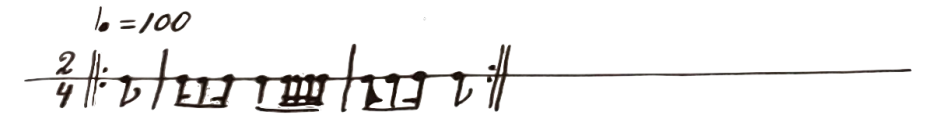
\includegraphics[width=100mm]{./imgs/img1.jpg}
%\caption{}
%\end{minipage}
\end{figure}

As fusas eram obtidas pelo esfregar do dedo polegar nos pandeiros.

Dos instrumentos, só era digno de nota o reco"-reco, duma forma e
principio sonoro que eu ainda não conhecia. Se compunha dum purungo
comprido, que fôra ou destampado na sua base, ou então perfurado em dois
orificios laterais, mais ou menos duns cinco centimetros de diametro
cada. No sentido do comprimento do purungo se ajusta uma haste fina de
madeira, amarrada nas suas pontas com um barbante. Essa haste é toda
dentada, e nela se esfrega a baqueta segurada pela mão direita. O
purungo, no sentido do comprimento, se ajusta ao longo do braço
esquerdo, entre êste e o corpo, apoiando"-se no mamilo esquerdo, e seguro
na base, pela mão.

\begin{figure}[!ht]
%\begin{minipage}{0,4\textwidth}
\centering
 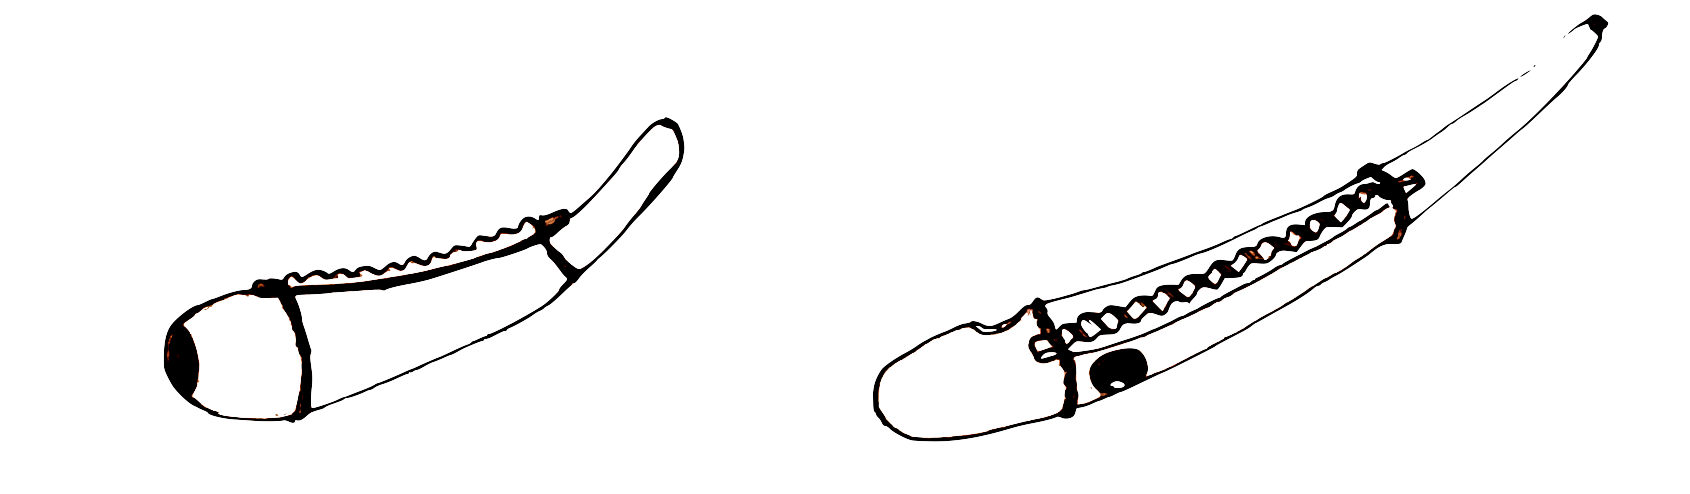
\includegraphics[width=100mm]{./imgs/img2.png}
\caption{Exemplos dos Recos de Carapicuíba.}
%\end{minipage}
\end{figure}

A Dansa da Santa Cruz tem seus versos tradicionais, guardados
imemorialmente desde tempos antiquissimos. Colhi algumas das quadras,
dum dos Camargos do lugar, pois que Carapicuíba foi feudo dos Camargos,
que aí se acoitavam, nas suas brigas com os Pires. Este Camargo vivo os
conhecia desde os tempos em que principiou a participar da dansa da
Santa Cruz, ha quarenta e tres anos passados. A quadra de salvação que
se entôa diante da porta da igreja, diz assim:

\begin{verse}
Deus te salve casa santa,\\
Aonde os santos têm morada,\\
Aonde está o calix bento\\
E a hóstia consagrada!
\end{verse}

Eis algumas quadras de salvação em frente das cruzes:

\begin{verse}
Deus te salve, cruz bendita,\\
Filho da Virgem Maria,\\
Em louvor ô (ao) vosso nome\\
Festejamos vosso dia!\\[5pt]
Viva nossa Santa Cruz,\\
Viva tambem São Joao,\\
Protejei os seus devotos\\
Que cumpre a devoção!\\[5pt]
Deus te salve, cruz bendita,\\
Consagrado, santo lenho,\\
Onde foi crucificado\\
Jesus Cristo Nazareno!\\[5pt]
Pelo sangue de Jesus,\\
Virgem Santa estremecida\ldots{}\\
Protegei os seus devotos\\
Fostes por Deus escolhida\\[5pt]
No carvalho junto à cruz,\\
Com alma de dor ferido\ldots{}\\
Jesus Cristo verdadeiro,\\
Perdoai ao arrependido\ldots{}\\[5pt]
Do céu caiu um cravo,\\
No braços de Santa Cruz,\\
Do cravo nasceu a Virgem,\\
Da Virgem nasceu Jesus.\\
\end{verse}

Eis quadras, de despedida, diante de cada cruz:

\begin{verse}
Vamos dar a despedida,\\
Como se costuma dar\\
Amanhã por estas horas,\\
Voltamos te visitar.\\[5pt]
Vamos dar a despedida,\\
Como deu o sabiá;\\
Amanhã por estas horas\\
Estarei neste lugar.\\[5pt]
Vamos dar a despedida,\\
Como deu Cristo em Belem;\\
Vamos todos dar um viva,\\
Até pro ano que vem!\\[5pt]
No último dia da festa\\
Vamos despedir da cruz\\
Que nos dê vida e saúde,\\
Para sempre amem Jesus.
\end{verse}

Estas duas últimas quadras só são ditas no terceiro dia, no fim da
noite, quando, depois dos dansados diante de todas as cruzes, se está de
novo salvando o cruzeiro do centro da praça. Outras quadras profanas,
iniciadas pelo verso"-feito tradicional, já se imiscuíram nas despedidas
ás cruzes. Como esta, por exemplo, que tambem colhi:

\begin{verse}
Vamos dar a despedida,\\
Como se costuma dar;\\
Não sinto a minha ida,\\
Como sinto te deixar.
\end{verse}

No caso, a rima dupla parece ser meramente casual.

Todas essas quadras e muitas outras, de sentido religioso, que não pude
colher pelas condições em que estava, são cantadas no início de cada
dansado e não durante o dansado propriamente. Durante êste, as quadras
são na generalidade profanas, e ás vezes comicas. Eis tres, me dadas
ainda por pessoas da familia Camargo, sendo que a primeira, um deles
trouxe de Jacareí.

\begin{verse}
Me mandáro uma laranja\\
Que (sic) a doçura me matou:\\
Si a laranja me mata,\\
Que fará quem me mandou!\\[5pt]
Numa mesinha redonda\\
Com uma menina joguei;\\
Jogando com ela, perdi;\\
Perdendo mesmo, ganhei.\\[5pt]
Sentei na beira do rio,\\
Para vê a agua correr;\\
Atirei ũa pedrinha nele,\\
Fez: Tim"-gum!
\end{verse}

O mais curioso na Dansa da Santa Cruz é a coreografia. Os cantadores com
suas violas e o resto da orquestrinha, formam uma linha reta na frente
da porta da igreja. Atrás deles em linhas sucessivas estão dispostos os
outros dansadores. Primeiro se tem de salvar a igreja, pedir licença pra
dansar e se despedir dela. Nessa parte do rito, embora não haja
proibição atual, são rarissimas as mulheres que tomam parte. Si uma
ainda apareceu e só nesse pedido de licença inicial diante da igreja,
nos outros pedidos de licença diante de cada cruz, não vi nenhuma. É
possivel que a tradição primitiva proibisse a participação feminina
nessa parte propriamente religiosa da coreografia. Mas não posso
garantir nada. Os instrumentos principiam tocando. Depois de bem fixo o
ritmo e a tonalidade, o puxador entôa uma quadrinha de louvação, do
gênero da primeira que dei. Não a entôa completa. Diz apenas os dois
primeiros versos, no fim dos quais o grupo todo entôa a firmata no
acorde de tonica, como já indiquei. Terminada a firmata, todo o grupo
faz um movimento de recúo, em passo simples, se afastando o mais
possivel da igreja. Esse passo porém é executado com o corpo meio
curvado prá frente, e implica ainda um movimento de oscilação de torso e
cabeça, que a cada passo, se curvam prá frente e se erguem, numa especie
de estilização do cumprimento. Depois de afastados, sempre na mesma
ordem de linhas de dansadores postadas umas atrás das outras, o grupo
todo avança, sempre no mesmo passo e atinge de novo o lugar inicial,
junto da porta da igreja. É então que o cantador conclúi a quadra,
seguido sempre do acorde coral. Isso se repete por várias vezes, sem
modificação coreográfica. Ás vezes apenas, durante os avanços ou recúos,
o cantador dá uma volta sobre si mesmo, no que é imitado por todos.
Outras vezes, durante os avanços, em vez de seguir normalmente até o
ponto de partida, o cantador torna a recuar de sopetão, o que ocasiona
atropelos, choques de corpos e procurada comicidade. Pra terminar,
depois do último avanço que deixou todos na posição e lugar inicial, o
cantador com a primeira fila, feita pelos instrumentistas, fazem
meia"-volta, encarando o resto dos dansantes. Tudo para. Está pedida á
igreja a licença pra dansar, e estão todos despedidos dela. Todo êste
rito se repete integralmente outra vez, diante do cruzeiro da praça. E
se repetirá sempre diante de cada cruz de flores. É só depois do pedido
de licença ao cruzeiro, que se forma a primeira roda de dansa. Um grupo
de mulheres, contadas geralmente entre as milhores dansarinas, se posta
na frente dos cantadores e da orquestrinha, á distância duns dois
metros, formando pares. O resto da população forma, continuando as duas
filas, a exterior de homens, a interior de mulheres, uma enorme roda, e
o dansado principia, movendo sempre prá direita. O ritmo é sempre o
mesmo. O passo coreográfico é apenas um, sempre o mesmo durante todos os
dansados das tres noites. Consiste no seguinte: As filas estão em ordem
de marcha, quero dizer, cada dansarino voltado na direção em que a roda
vai se mover. Com o pé esquerdo, os homens dão um passo prá frente,
concluindo o passo todo com o movimento de avanço do pé direito. Apenas
êste não deu um passo inteiro, que o colocaria mais adiantado que o
esquerdo: deu meio passo e se colocou exatamente junto do esquerdo.
Então êste, num movimento circular, executa pra trás um quarto de passo,
de forma que fica enfrentando não mais o companheiro do mesmo sexo que
lhe está na frente, mas o par feminino da outra fileira. E o pé direito
então, com um pequeno movimento de recúo e mudança de direção, vem se
colocar de novo junto do esquerdo e na direção dêste. Assim, agora
mulher e homem se enfrentam. Esse é o passo. O corpo, como no rito
anterior, se mantem sempre levemente curvado, a cada movimento dos pés
fazendo uma oscilação leve de quem está cumprimentando. O tique
caracteristico do dansado, sistemático, e só realizado bem pelos bons
dansarinos da dança da Santa Cruz, consiste num movimento bastante
dificil de descrever literariamente. Quando o pé esquerdo recúa o seu
quarto de passo circular pra enfrentar a mulher, a perna direita em que
o corpo está se equilibrando no instante (e que fizera uma leve
curvatura de joelho quando, no passo anterior, o pé direito se apoiara
no chão) se inteiriça com certa rapidez, de forma que o corpo se
suspende um bocado mais. O dançarino aproveita êsse movimento de
alteiamento do corpo, pra jogar a bunda pra trás. Toda esta movimentação
aliás é sempre discreta, e consegue ser granciosissima nos bailarinos
bons. A mulher executa exatamente a mesma coisa, fazendo com o lado
direito do corpo o que o homem faz com o esquerdo. E êste passo se
repete infindavelmente. Para reinicia"-lo cada vez de completado, no
momento em que homem e mulher se enfrentam, o pé esquerdo pra adquirir
de novo a posição primitiva é obrigado a fazer um movimento de novo de
quarto de círculo, mas prá frente. Ás vezes, quando um grupo de
dansadores da roda, ou apenas um par, se entusiasmam demais, principiam
gingando com movimentos laterais de quadris e passos mais largos e de
repente o par, ou o grupo, dá uma volta balanceada e aspera, cada
individuo girando sobre si mesmo.

Durante o dansado, surgem na roda enorme, novos grupos de cantadores
desprovidos de instrumentos. O mestre da dansa com seu acompanhador
vocal e sua orquestrinha que não para nunca de bater o ritmo, tira,
sempre bipartida e acompanhada das firmatas corais, a sua quadra
profana. Quando esta termina, noutro lugar da roda outros cantadores
tiram outra quadra. E são depois outros e depois outros, de forma que,
nos momentos de grande animação, a cantoria é ininterrupta e o dansado
se prolonga sempre lerdo sempre monotono. Mas todos estão delirando
de\ldots{} prazer paulista, sêco, e se diria tristonho. É a base de indio. A
dansa de Santa Cruz atualmente é dansada por toda uma população
variegadissima que vem ás vezes de leguas longe, dos arredores de
Carapicuíba. Vi caipiras carijós, negros, mulatos, portugas, intalianos
e japões, sim, até japoneses! fazendo a roda da Santa Cruz. Mas da dansa
monótona, sombria mesmo, vinha um rescaldo tão vivo ainda de indiada,
que chegava a assombrar. Nunca tive em minha vida uma impressão assim
tão direta, tão convencida de herança amerindia, como diante dessa dansa
da Santa Cruz. Si é certo que o ambiente multissecular de Carapicuíba me
transportava pra tres seculos atrás, creio ter conservado o espirito em
bastante nitidez de julgamento e justiça, pra que essa impressão me dada
pela dansa não fosse uma fantasia de peito incendiado pela tradição. O
coração queimava sim, mas o juízo se mantinha friamente etnográfico.
De"-fato, não lembro nada nem das descrições, nem das fotografias nem dos
filmes de dansas africanas, e muito principalmente das coreografias que
os Africanos truxeram pra cá, nada conheço que se assemelhe
essencialmente á dansa da Santa Cruz. Em compensação, nas descrições de
dansas amerindias do Brasil, nas gravuras, e principalmente num dos
filmes do general Rondon, bem como nos fonogramas do Museu Nacional,
encontro elementos que me permitem, tanto musical como
coreograficamente, ver na dansa da Santa Cruz, de Carapicuíba, uma
tradição perfeitamente amerindia, fortemente conservada e viva ainda.
Tudo leva a crer, a lição da História como o estado de absoluto atraso e
insulamento em que vegeta o vilejo (que nem é ponto de passagem de
nenhuma rodovia estadual), tudo me leva a crer que a dansa da Santa Cruz
seja ainda um remanescente dos primeiros seculos, uma daquelas festanças
de Indio que os jesuitas adotaram na catequese, lhe modificando apenas o
rito e os textos, na direção do Catolicismo.

\begin{flushright}
\vfill
Mário de Andrade

S. Paulo, 7 de maio de 1935
\end{flushright}


\chapter*{Moçambique}
\addcontentsline{toc}{chapter}{Moçambique, \emph{por Mário de Andrade}}
\hedramarkboth{Moçambique}{}


\section*{(Cantos e Dansas, recolhidos do natural, em~Santa~Izabel, Estado
de São Paulo.)}

Entre as diversas dansas"-dramaticas de negros, tradicionalizadas no
Brasil e conservadas até os nossos dias, ha o \emph{Moçambique}, que a
gente rural paulista pronuncia tambem \emph{Maçambique}. Tive ocasião de
assistir a êste bailado, na pequenina cidade de Santa Izabel, a 50 e
tantos quilometros da capital de São Paulo, pela festa do Espirito
Santo, de 1933. Pelo menos aqui no Estado, a festa do Espirito Santo é
sistematicamente aproveitada pelos ranchos de negros, ou já
exclusivamente de caipiras, pra dansarem seus bailados, \emph{Congos,
Moçambiques, Caiapós.} Em Santa Izabel dansava"-se qualquer dêstes tres,
sendo que o \emph{Congado} (por aqui se diz exclusivamente
\emph{Congado}, e não \emph{Congos}, como no Nordeste) diferia do
\emph{Moçambique} apenas por haver, no acompanhamento instrumental, um
instrumento polifonico, a viola, e algum entrecho. Vai aqui tudo quanto
pude observar no \emph{Moçambique} de Santa Izabel.

O \emph{Moçambique} não tem propriamente entrecho dramatico nenhum, e se
identifica por isso com os \emph{Maracatús} pernambucanos. É exatamente
um cortejo que, em certas festas do ano, vagueia pelas ruas, parando pra
dansar na frente de certas casas. Esse cortejo partilha de todo o
cerimonial, extra muros, da festa religiosa. Acompanha o Imperador do
Divino em suas perambulações, acompanha procissões, etc. Certamente, no
tempo de dantes, dansaria no adro das igrejas, ou mesmo dentro destas ---
coisas já proibidas agora pelos padres. Quando cheguei em Santa Izabel,
o rancho do \emph{Moçambique} estava no adro da matriz esperando o fim
da missa. Acabada esta, foi acompanhar o Imperador até a casa dele, e na
frente dela dansou. De"-tardinha escutei o Rei falar que careciam ir
tirar as vestimentas de dansa, pra acompanharem a procissão. Alem disso,
como se verá da descrição, a religiosidade catolica está completamente
misturada com êste bailado, da mesma forma com que se alia ainda aos
\emph{Congados}, do Centro, e aos \emph{Maracatús}, do Nordeste.

O rancho se compunha, no total, duns trinta individuos. Todos machos,
(não ha bailarinas, como nos \emph{Maracatús}), com excepção da Rainha,
e das duas porta"-bandeiras, que eram caipirinhas novas. Na grande
maioria eram totalmente brancos, caipiras legítimos. O proprio chefe (o
Mestre) dos instrumentos, diretor experimentado, ensinador de tudo,
ensaiador das dansas, dirigindo no seu instrumento a percussão
acompanhante, era caipira, sem traço de sangue negro.

\section*{Personagens e Indumentaria}

\versal{O REI} --- Era um negro velho, de raça provavelmente pura. Todo de
branco, apenas a camisa e calça de trabalho, lavadas. Sobre a cabeça
tinha um lenço verde, de que uma das pontas lhe caía sobre a testa.
Sobre o lenço estava imposta a corôa dourada. Na mão uma especie de
ceptro.

\versal{A RAINHA} --- Tambem uma negra velha, bem arranjadinha, toda de
branco. A tiracolo uma estreita fita azul, terminando em laço pendente,
na anca direita. Na cabeça uma dessas corôas pequenas, com florzinhas
prateadas e fios de prata, usadas comumente pra enfeitar anjos e virgens
de procissão. Nas mãos uma pequena salva de vidro, pra colher esmolas.

\versal{2 PORTA-ESTANDARTES} --- Moças sem distintivo algum na
indumentaria, carregando as figuras de Santo Antonio e da Senhora do
Rosario, em pinturas populares. Os dois estandartes estavam
abundantemente enfeitados com flôres de papel.

\versal{OS MOÇAMBIQUES} --- São os figurantes do bailado. Todos com roupas
brancas, camisa e calça, ou de riscadinho miúdo, já desbotado do Sol e
das lavagens. O tom procurado era mesmo o branco. Tambem nos Congados,
tanto de Minas como de São Paulo, a côr geral procurada é o branco; no
que os bailes daqui diferem fortemente dos de todo o Norte, onde o
branco é esquecido, a não ser, e obrigatoriamente, pela maruja de certos
reisados. Na barra da calça, num courinho que a aperta, está prêso o
\emph{conguinho}, pequeno caracaxá de lata. A indumentaria especial dos
Moçambiques consistia exclusivamente no chapéu, no bastão, e na pala.
Esta, ao feitio das palas femininas, era amarrada por uma fita no
pescoço. E sôlta, circular, terminando na altura do ombro. Da mesma
forma que o chapéu, a pala é decorado fantasistamente, á vontade do
freguês. As côres não eram obrigatorias, e havia palas verdes, pretas,
azúis. Uma, duas fitinhas de côr diferente, corriam, costuradas, junto á
borda da pala. Algumas palas traziam tambem estrelinhas prateadas, ou
pequenos laços de fita ou de papel"-de"-seda colorido, dispostos sem ordem
fixa. O bastão, de pau roliço, terá pouco menos de metro. A dois terços
do comprimento é perfurado, e pelo orificio passam um amarrilho, do qual
pendem muitas fitinhas estreitas de côr variada. O chapéu é uma especie
de fez, de pouca altura, tambem com liberdade completa de decoração.
Sobre o fundo, indiferentemente branco, vermelho ou preto, colam
serpentinas ou costuram fitas de outras côres. Alguns eram decorados com
rendas douradas, outros tinham lacinhos e pufes, um mesmo era tomado
completamente, sobre o fundo vermelho, por um entremeio de chochê.

\section*{Instrumentos}

No \emph{Moçambique} é usada sistematicamente a percussão. Havia caixas
de dois tamanhos e duas \emph{pernangumas}. A \emph{Pernanguma}, ou
\emph{Prananguma} como pronunciou um dos caipiras, como nome e forma
jamais eu vira. É um instrumento do mesmo princípio acustico do ganzá,
mas diferindo completamente dêste pela forma. Consiste numa lata
redonda, chata, duns trinta centimetros de diametro, contendo chumbo
dentro. Fecham a lata com os chumbinhos dentro, soldam"-a completamente e
lhe ajuntam duas alças por onde o instrumentista pega o instrumento e o
move. Como se dá com os\ldots{} virtuoses do ganzá, o tocador da pernanguma
sabia tirar do seu instrumento muitos ruídos diferentes, chiados suaves
com o correr lerdo do chumbo, pancadas violentas, pancadas mais suaves.

\section*{O BAILADO}

O bailado, concebido no conceito da Suite, se prolonga indefinidamente,
sem ordem predeterminada de dansas, e nem mesmo ordem obrigatoria na
figuração coreografica de cada dansa. Os bailarinos mais habeis, que são
os quatro da frente, mudam de figuração quando querem, e o resto do
cordão os segue. Entre um e outro número de dansa, tem sempre uma
louvação aos santos, de tipo responsorial, solo e côro, e sob o
princípio do recitativo. Este recitativo, não é propriamente cantado, é
gemido, é por assim dizer, queixado. O solista o entoa botando a mão ao
lado da boca ou mesmo sobre ela, e produz voluntariamente um som
fanhoso, completamente diverso do das melodias das dansas, que êste é
franco, produzido só pela boca. Essas louvações, de pouco interesse
melodico, são porêm de grande curiosidade de entoação. O canto lúgubre
produzido pelo solista e pelos respondedores, na sua incrivel indecisão
linear, se assemelha ás vezes vagamente a certas linhas de cantochão.
Provavelmente essas louvações serão inspiradas nos cantos de igreja, nos
te"-deuns, nas bênçãos do Santissimo, e principalmente en certas
dialogações entre oficiante e côro nas missas cantadas, e nas ladaínhas.
Mas evocam invencivelmente a escravidão, e aqueles tempos, nas fazendas,
em que as rezas dos senhores eram respondidas com os amens e sicuteras
indiferentemente fatigados dos escravos. A indiferença, a falta de
controle intelectual ou de sentimento, com que êsses louvores são
entoados, é total. Por outro lado, é curiosissimo notar que tais
louvações se identificam absolutamente com os recitativos que nos
batuques rurais do Centro do país (pelo menos em São Paulo) são
intercalados entre um samba e outro. De resto, os processos de criação
musical e poetica, dos sambas paulistas que já pude observar, são os
mesmos que dêste \emph{Moçambique}. A diferença é mais de textos, que
nos batuques, como nos seus recitativos intermediarios são profanos e no
geral improvisados, ao passo que no \emph{Moçambique} são religiosos,
vagamente tradicionais, ou se relacionando com a parte representativa do
bailado. Eis um texto de louvação, sistematicamente repetido neste
Moçambique:

\begin{verse}
Solo: --- Valei! Valei Nossa Sinhóra du Rusaro!\\
Côro: --- Ai, (ou Ei) meu Deus!\\
Solo: --- Valei"-me Santo Bastião!\\
Côro : --- Ai, (ou Ei) meu Deus!
\end{verse}

Tambem, como nos sambas paulistas, enunciada a melodia da dansa pelo
solista, o côro, conforme a disposição estrofica, ou repete
integralmente a melodia ou a completa com alguma resposta. Mas desde que
a estrofe se complete, o texto será repetido sempre o mesmo, sem
variação alguma, durante todo êsse número de dansa, 30, 40 vezes. De
resto, pelo menos êste \emph{Moçambique} de Santa Izabel era
musicalmente e poeticamente pauperrimo. Quasi todos os números foram
cantados com a mesma melodia (Melodia nº~1) ou com as outras duas que vão
aqui. Não ouvi usarem de outras melodias.

A coreografia, sim, era bastante rica --- justo pois a parte mais dificil
de registrar literariamente. Originalidade de movimentação de pés, muita
variedade de transladação e combinação de movimentos coletivos, muita
variedade de jeitos de corpo e de valimento do bastão.

A disposição geral é a mesma dos ranchos e bailados do país. O cortejo
se organiza, indo na frente os dois porta"-estandartes, em seguida o par
do Rei com a Rainha, em seguida os instrumentistas, e atrás os
bailarinos, tudo a dois de fundo. Quando param pra dansar, os
porta"-estandartes se voltam pros bailarinos, bem como o Rei e a Rainha,
êstes se dispondo indiferentemente, ao lado ou na frente dos
estandartes. Os instrumentos se colocom a um lado, junto dos personagens
principais.

Inicialmente os bailarinos, nas suas duas fieiras, se defrontam. Em
quasi todas as dansas, apesar dos bailarinos serem todos homens,
permanece a noção coreografica do par. O primeiro bailarino relacionará
sempre a sua dansa pessoal com a do companheiro do lado, e ambos
relacionarão as suas figurações, os seus ``\emph{manejos}'' como êles
falavam, com a do par fronteiro. Algumas vezes porêm o círculo fecha, e
as dansas continuarão numa roda que gira.

Eis algumas dansas que consegui colher, sempre reconhecida a quasi
impossibilidade de descrever com exatidão a coreografia.


\begin{figure}[!ht]
%\begin{minipage}{0,4\textwidth}
\centering
 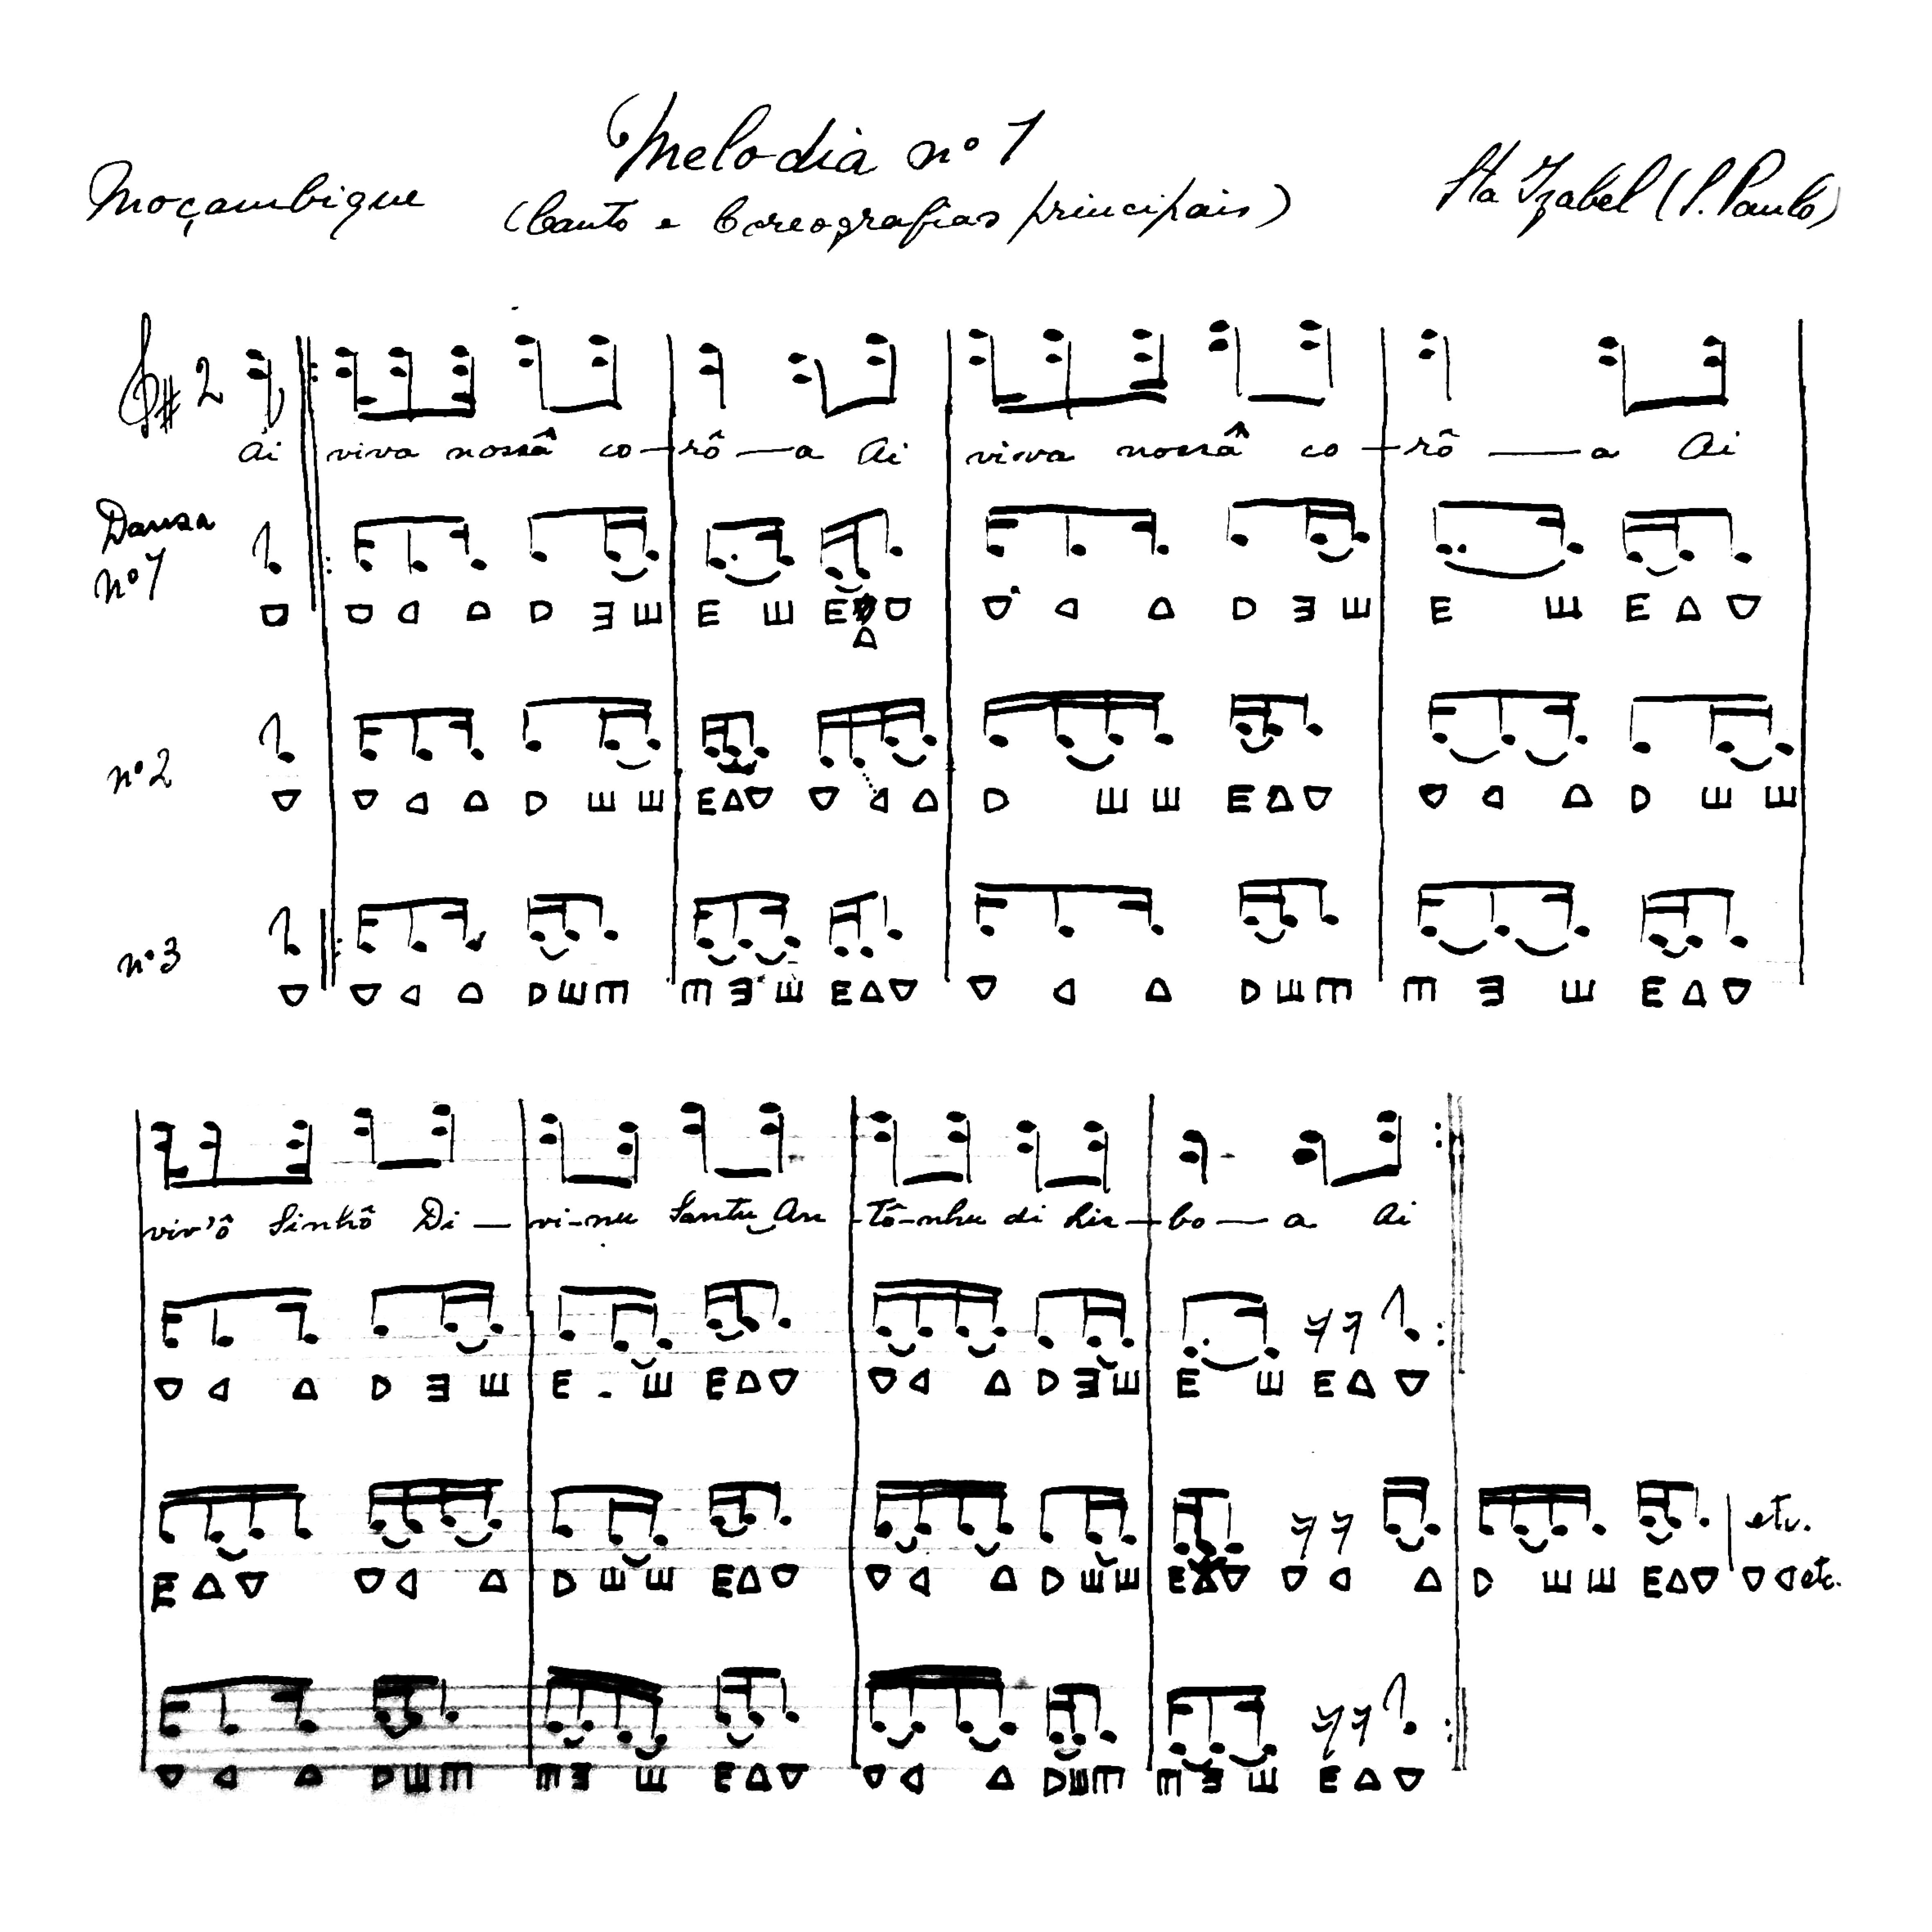
\includegraphics[width=100mm]{./imgs/img3.png}
\caption{\versal{DANSA Nº~1}.}
%\end{minipage}
\end{figure}

\begin{verse}
Ai viva nossa corôa!\\
Ai viva nossa corôa!\\
Ai viv'o Sinhô Divino,\\
Santo Antônho de Lisboa!\\[5pt]
(O côro repete integralmente a estrofe.)
\end{verse}

\section*{Explicação das grafias coreograficas}

Na verdade essas tres grafias coreograficas não passam de variantes umas
das outras. A variante nº~3, que é a mais simples e mais lógica, e que
por isso poderá se considerar como protótipo, foi no entanto a que vi
executada menos vezes. As outras duas foram mais repetidas e, apesar da
fadiga que causa á perna esquerda, a de mais preferencia, não só por
mais repetida como porquê despertava maior entusiasmo nos bailarinos,
foi a de nº~2.

O sinal D indica o pé direito. O sinal E indica o pé esquerdo. D e E
representam os pés quando pousados no chão e sustentando o pêso do
corpo. \rotatebox[origin=c]{180}{D} e \rotatebox[origin=c]{180}{E} representam os pés quando em pausa, erguidos junto ao
outro pé que pousa, e imoveis. \rotatebox[origin=c]{90}{D} \hspace{.1pt} e \rotatebox[origin=c]{90}{E} \hspace{.1pt} representam os pés quando
transladando"-se da pausa, ou obliquamente prá frente ou pra trás, ou
então lateralmente. \rotatebox[origin=c]{270}{D} e \rotatebox[origin=c]{270}{E}  representam os pés batendo com a planta
inteira no chão, e fazendo, pois, soar os conguinhos.

Quando o solista entoa a melodia, os dansarinos estão imoveis. Enunciada
a melodia completa, os dansarinos a repetem, completamente ainda e
sempre imoveis. E essa imobilidade espectante continua até que o ritmo e
o texto se fixem bem. Quando a cantoria está mesmo bem fixa, o que
chamarei de Primeiro Bailarino abre a dansa, e os outros, que estão
reparando nele, o imitam imediatamente. Não tem apito nem outro processo
nenhum de determinar a mudança dum manejo pra outro.

\section*{Coreografia nº~3}

Fixada a cantoria, todos, que estão com os dois pés pousados no chão, á
primeira colchêia em arsis da melodia, batem com o pé direito no chão.
Ao tempo forte seguinte tornam a bater com o mesmo pé e o erguem um
centimetro do chão, em pausa mais ou menos de colchêia, figurando assim
a síncopa do primeiro tempo com uma pausa do pé direito erguido. Á
última semicolchêia do primeiro tempo executam um movimento de
translação dêsse mesmo pé, ou lateralmente prá direita, ou obliquamente
prá frente; neste último caso, visando se aproximar do bailarino da fila
fronteira, e que estava distante no início da dansa apenas uns tres
metros. (Como os movimentos laterais não implicam sinão um ir e vir
lateral do bailarino, não o indicarei mais. Escolhidas as traslações
laterais, elas se repetem infindavelmente até o primeiro bailarino
iniciar algum manejo novo.)

Feito o movimento de translação oblíqua prá frente do pé direito, êste
pousa no chão á primeira semicolchêia do segundo tempo do compasso. Á
segunda semicolchêia, o pé esquerdo, que ficara á distância de passo do
direito, translada"-se pra junto dêste, e, á colchêia que completa o
compasso, bate no chão. É pois agora o pé esquerdo que bate no chão, e
em nova batida inicia o compasso seguinte. Este será absolutamente
identico ao primeiro, como figuração coreografica, apenas o que foi
feito com o pé direito no primeiro compasso, é feito agora pelo esquerdo
e vice"-versa. E como o bailarino fez novo movimento de traslação prá
frente, agora êle está junto do bailarino da fila fronteira --- o que
quer dizer que as duas fieiras estão perfeitamente unidas agora, no
centro do terreno em que se dansa. O terceiro e quarto compassos são
absolutamente identicos aos dois primeiros, só que agora os movimentos
de translação, em vez de serem prá frente, são pra trás, os bailarinos
voltando pois de costas, ao lugar em que estavam no início. E como a
melodia comporta ainda mais quatro compassos pra completar a quadratura,
temos que os dansarinos ainda executarão mais um\ldots{} manejo completo de
ir até junto do dansarino fronteiro e voltar ao lugar inicial.

\section*{Coreografia nº~1}

Trata"-se evidentemente duma variante apenas, e preferida, da coreografia
nº~3. A diferença consiste em que as duas batidas com o pé no chão, em
que os conguinhos soam mais vivos, são feitas sempre só com o pé
direito. Assim, na segunda metade do segundo tempo do primeiro compasso,
o pé esquerdo apenas se translada pra junto do pé direito e pousa de
leve no chão - ao acento forte da primeira parte do segundo compasso;
mas se ergue de novo, e faz novo movimento de translação obliqua prá
frente, pousando e recebendo o pêso do corpo no primeiro som do segundo
tempo. Então o pé direito se translada pra junto dele e executa de novo
as duas batidas no chão. Nos dois compassos seguintes todo êsse manejo é
repetido pra trás, os dansarinos voltando aos seus lugares primitivos.

\section*{Coreografia nº~2}

Esta coreografia foi a que vi mais numerosamente repetida. É a mais
dificil por contradizer muito o movimento natural do compasso binario.
Se observará, com efeito, que o dansarino executa um manejo que exige
tres tempos inteiros pra se completar --- o que faz com que só depois de
tres repetições da melodia completa, isto é, só depois de 24 compassos,
êle se encontre no movimento coreografico"-melodico inicial! A
movimentação é a seguinte:

O primeiro tempo do primeiro compasso é exatamente igual ao das outras
duas variantes. Depois do pé direito estar pousado de novo, o pé
esquerdo, na primeira metade do segundo tempo, executa, sem pouso
intermediario no chão, dois movimentos rapidos de traslação: o 1º na
primeira semicolchêia da segunda metade dêsse mesmo tempo, indo
obliquamente até bater ou quasi bater com o calcanhar no calcanhar do pé
direito pousado; e o 2º na semicolchêia final do compasso, afastando"-se
do pé direito, obliquamente, prá frente, e só então, na acentuação forte
do primeiro tempo do segundo compasso, pousando no chão e recebendo
sobre si o pêso do corpo. Já porêm na segunda semicolchêia dêsse tempo,
o pé direito se translada rapido pra junto do pé esquerdo, e, na
colchêia que acaba êsse tempo, executa a batida no chão pra soar o
conguinho. Na primeira colchêia do tempo seguinte bate de novo no chão,
perfazendo as duas batidas caracteristicas da coreografia. Assim, em vez
dum número par de tempos de compasso, foram necessarios tres tempos. E
outros tres tempos serão necessarios pra execução completa do mesmo
movimento, só que agora de recúo, pra voltar ao lugar inicial.

Esse é o movimento de pés do manejo principal do \emph{Moçambique,} e de
suas variantes. Mais dificil de figurar é o meneio do corpo. Resta aliás
observar tambem que o que chamei de ``passo'' e translação dos pés, era
um verdadeiro pulinho, havendo pois, no movimento de traslação pulado,
pequenos momentos, no maximo de semicolchêia em que o bailarino fica com
os dois pés no ar. E mesmo quando não se dava pulo, mas um verdadeiro
passo, êste em nada se assemelhava ao passo natural do andar, porquê o
dansarino, nos momentos de pouso, em que um dos pés executa as duas
batidas características no chão, curvava o joelho da perna
correspondente ao outro pé. E depois, nos momentos de translação de
qualquer dos pés, esticava o joelho recurvado na outra perna, formando
assim um movimento sucessivo de abaixar e erguer de corpo, ondulante,
assimilavel ao pulinho.

A postura natural dos dansarinos é de curvatura pra frente, o corpo
dobrado, nos figurantes mais habeis, nos rins, num ângulo muito
incisivo, de pouco mais de 90 graus. E como os joelhos, nas posições de
pouso, estão sempre flexionados, o bailarino de perfil é uma linha
quebrada de tres retas:

\begin{figure}[!ht]
%\begin{minipage}{0,4\textwidth}
\centering
 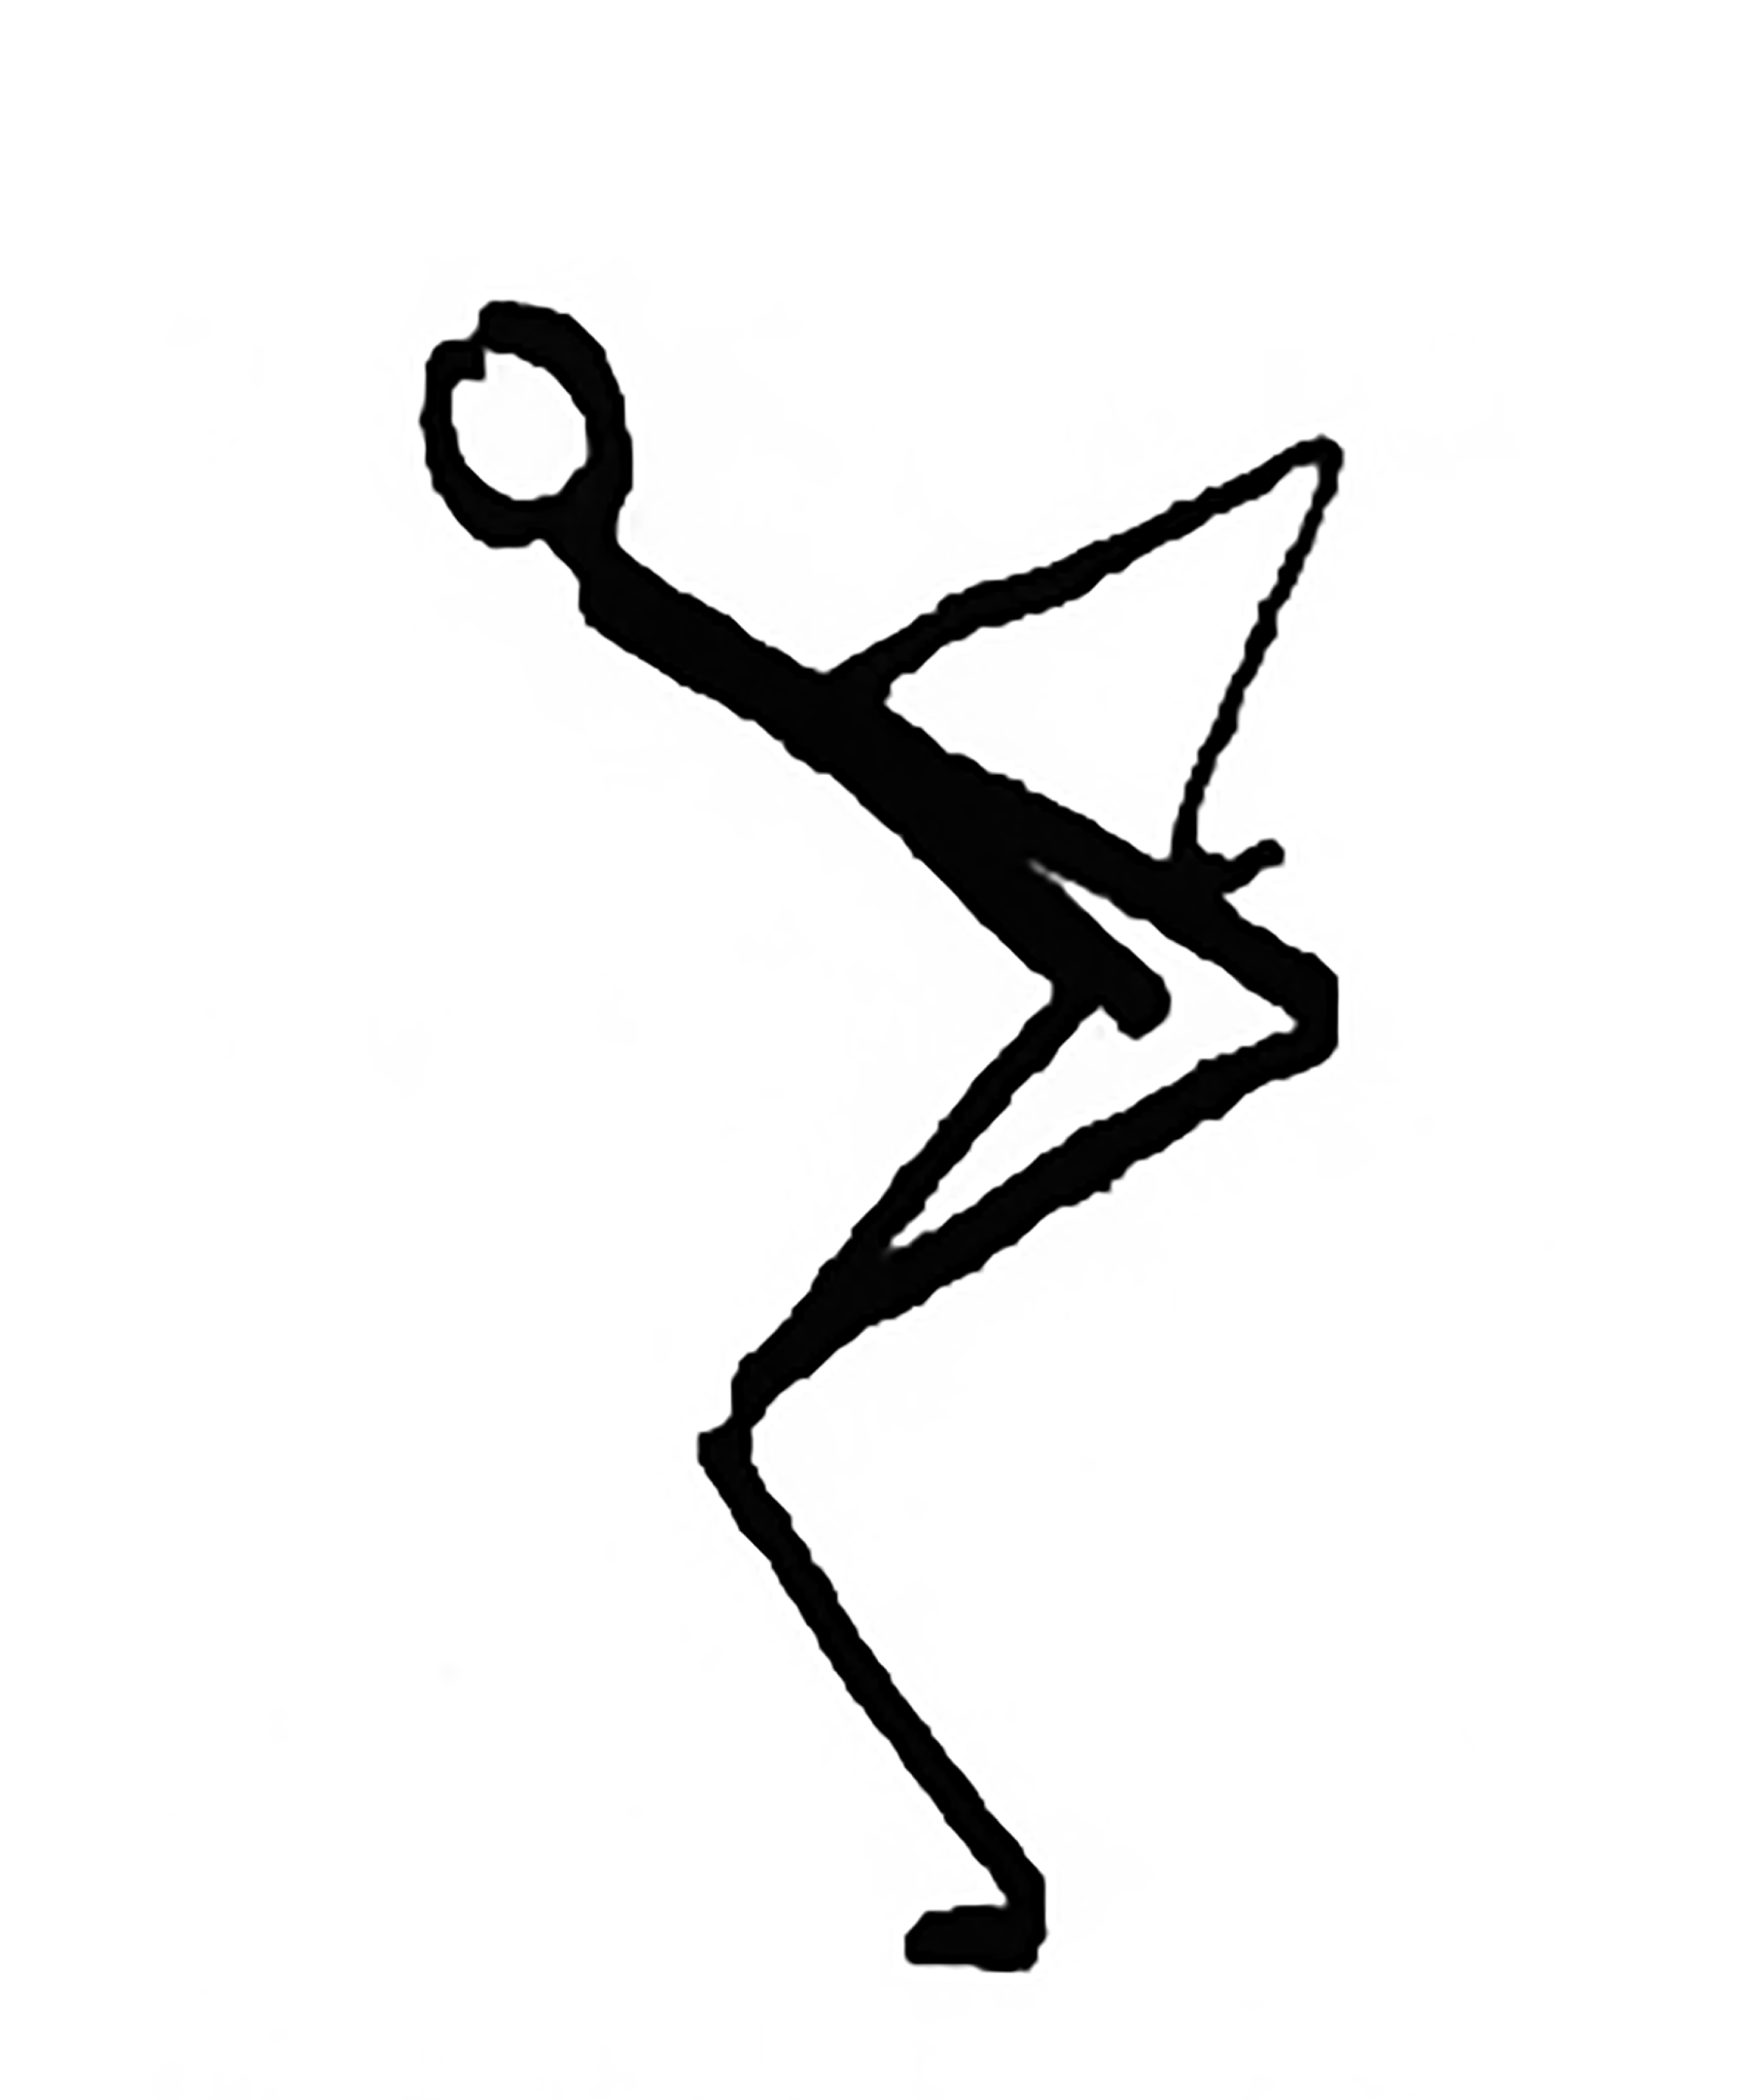
\includegraphics[width=16mm]{./imgs/img4.png}
%\caption{}
%\end{minipage}
\end{figure}

E, mesmo quando está junto do bailarino da linha fronteira, não executa
a embigada tradicional dos sambas, nem siquer a esboça. A embigada é
completamente desconhecida dêste \emph{Moçambique}.

Não porêm o movimento de ancas. Depois dos pulos ou passos, quando o pé
que vai sustentar o pêso do corpo, pousa no chão, os dansarinos mais
habeis faziam movimentos fortes de anca, na mesma direção da translação
que acabava"-se de realizar, levando a bunda nessa direção, em movimento
suave. Assim, o pé pousado não podia ficar inteiramente imovel, mas
praticava no chão um movimento rotativo, sempre dirigido na mesma
direção do movimento de anca. E os braços, quando não tinham coreografia
especial, se dobravam na cintura, onde apoiavam pelas costas das mãos.

Essas tres variantes do mesmo passo foram repetidas em quasi todas as
dansas, ora uma, ora outra, indiferentemente. Anoto agora as figurações
tomadas com êste primeiro texto:

1: Executam o passo, avançando e voltando ao lugar várias vezes. 2:
Depois disso, o primeiro bailarino, que é ponta de fila, se volta pro
companheiro que lhe está imediatamente ao lado na mesma fila, e o mesmo
fazem as figuras ímpares das duas fieiras. Assim, cada fieira realiza
agora, nitidamente, um grupo de pares, cada bailarino defrontando o seu
par. Cada par executa então o mesmo passo anterior, só que em
translações sempre prá frente, dando ao avanço do bailarino uma direção
circular, de forma que cada par gira sobre si mesmo:

\begin{figure}[!ht]
%\begin{minipage}{0,4\textwidth}
\centering
 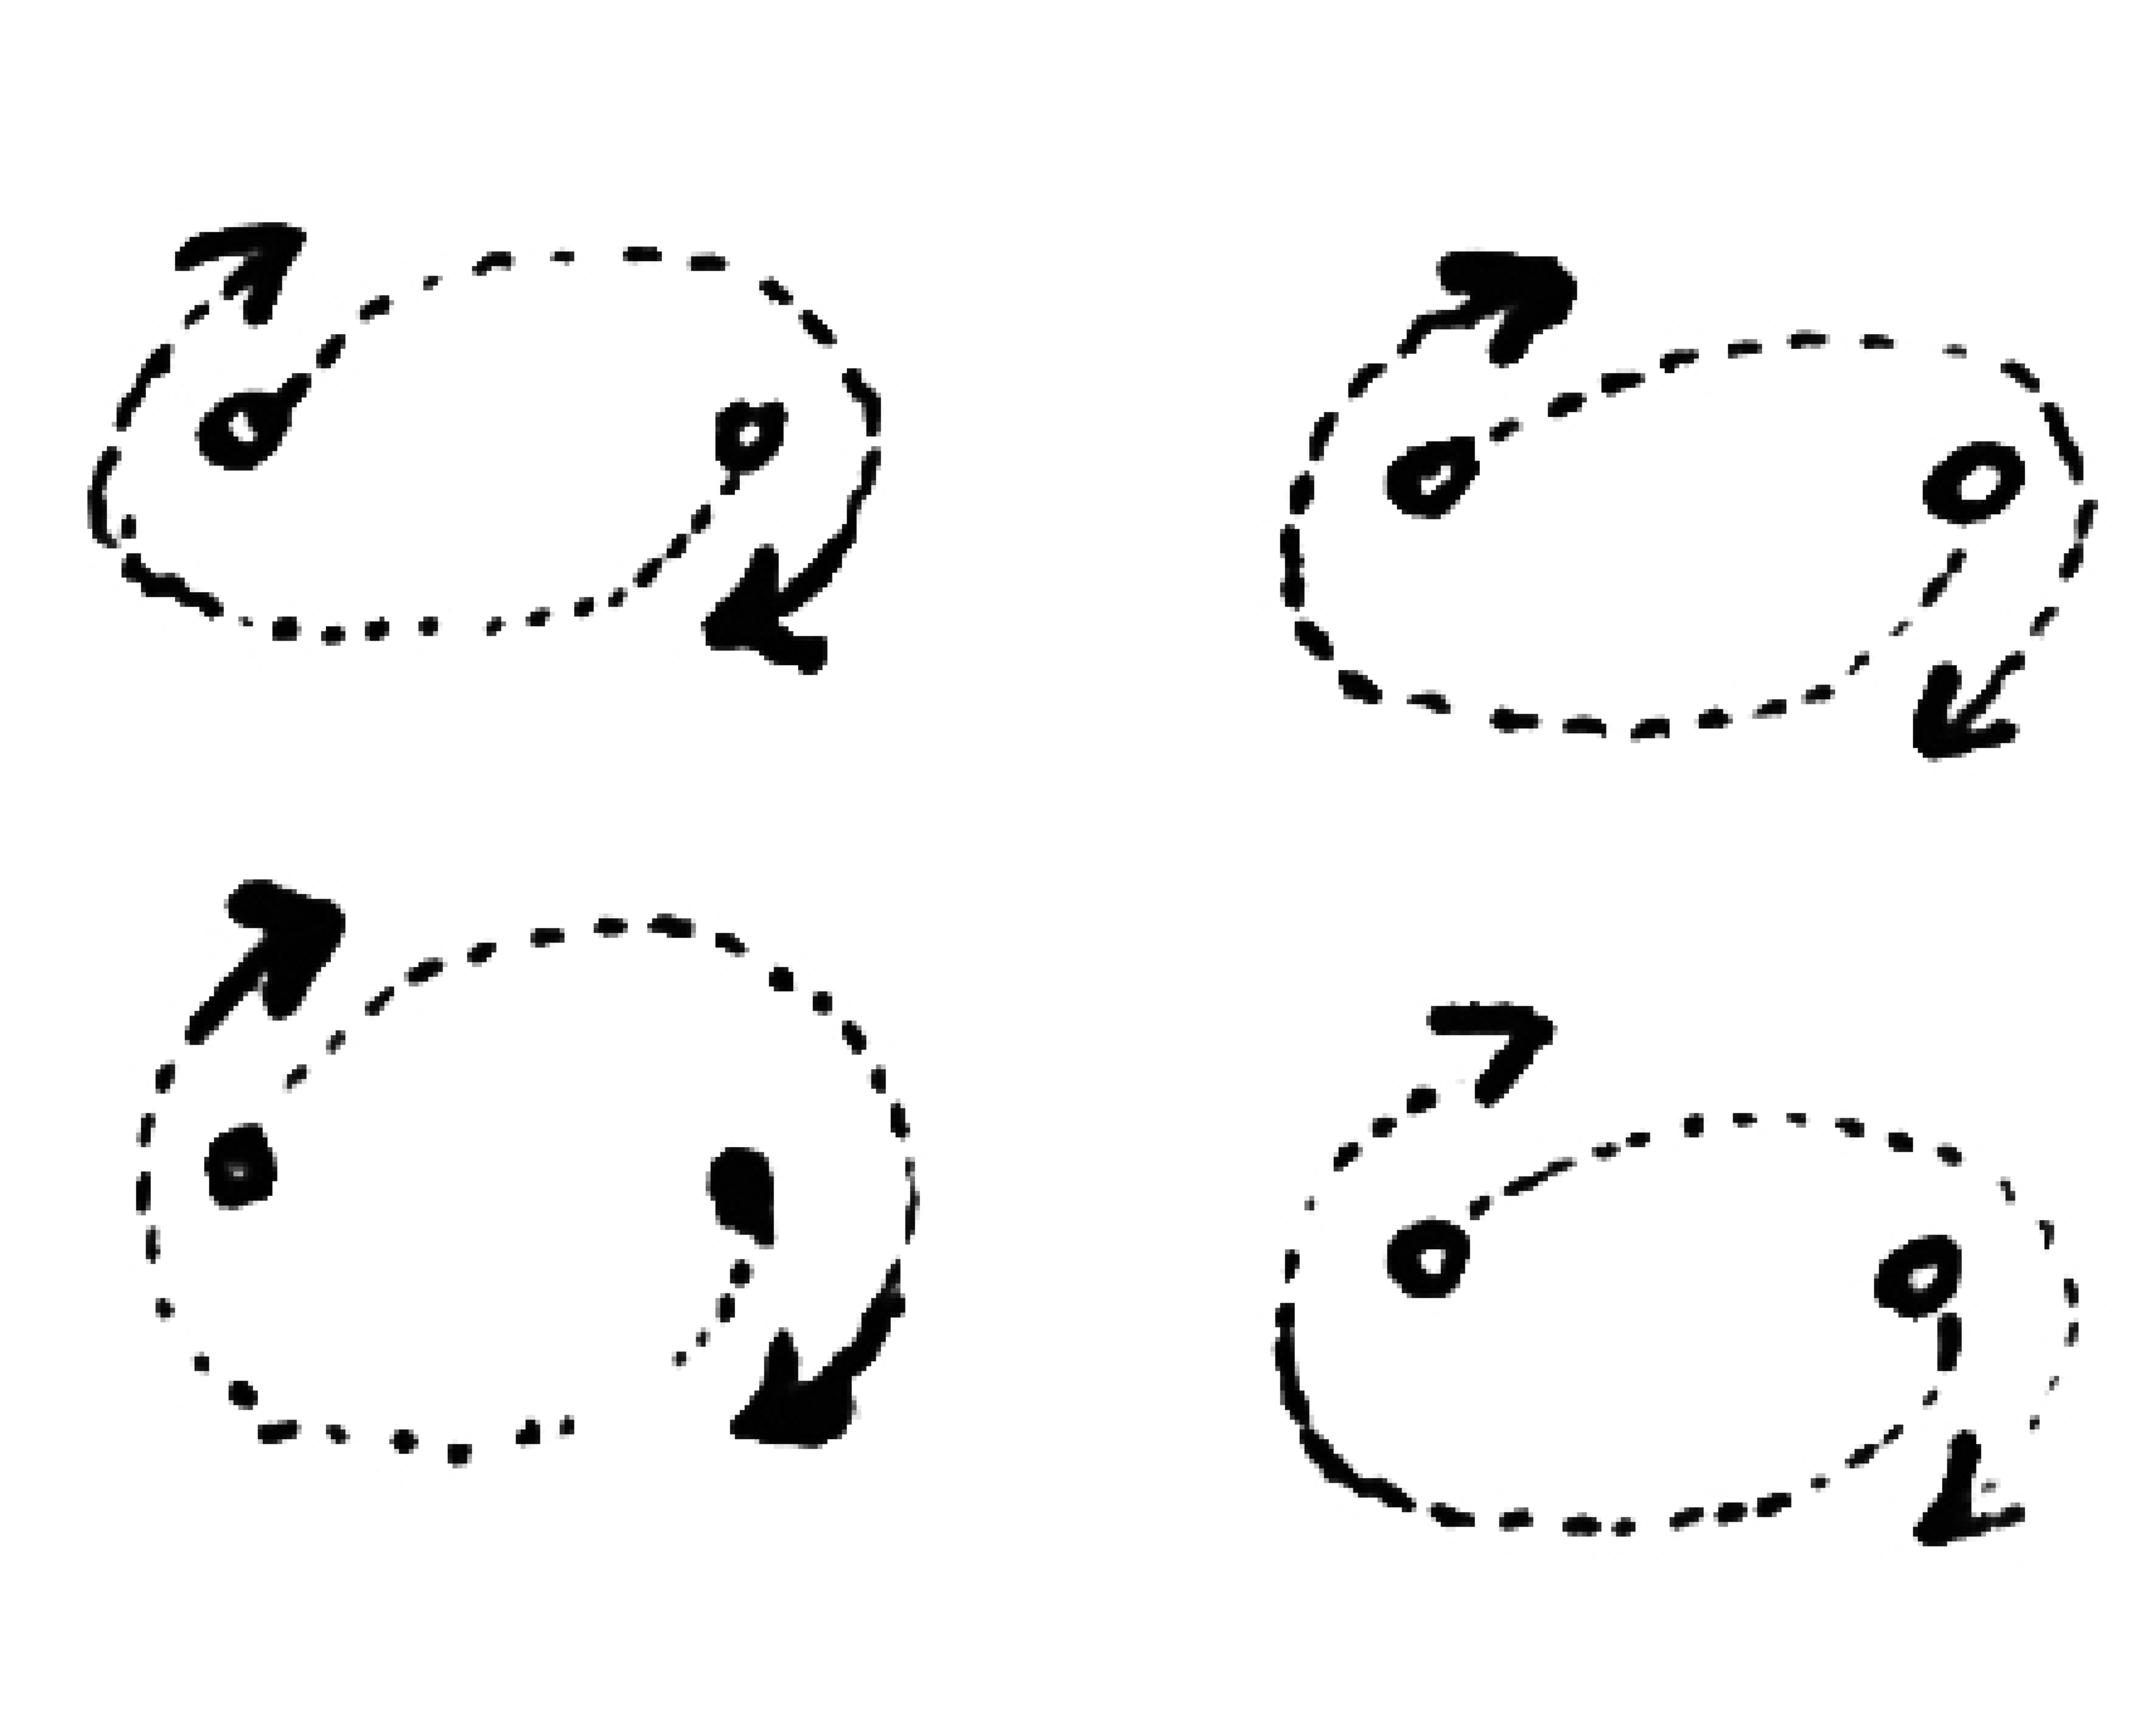
\includegraphics[width=30mm]{./imgs/img5.png}
%\caption{}
%\end{minipage}
\end{figure}

3: Executada essa figuração várias vezes, começa outra que consiste nas
duas filas do bailado se ligarem por suas extremidades, formando roda.
Mas sempre cada bailarino está voltado pro seu par, de forma que a roda
(que em qualquer das dansas girou sempre á esquerda; e todos os
movimentos de giro, tanto do bailarino sobre si mesmo, como dos pares
foram sempre executados prá esquerda) comportará sempre bailarinos que
avançam circularmente de costas, e seus pares, que avançam circularmente
de frente. Os de costas fazem aqui sempre só movimentos de translação
prá retaguarda, está claro.

Terminado o giro completo da roda e voltados todos os bailarinos aos
seus lugares iniciais, tudo parou.


\section*{DANSA Nº~2}

Mesma melodia da dansa nº~1. Texto:

\begin{verse}
Glorioso São Binidito,\\
Glorioso Santú Bastião!\\
Estí nossu patraozinho\\
Insinô nossús irmão!\\
\end{verse}
(``santú'' por santo; ``êstí'' por êste: deformações ocasionadas pela
acentuação ritmica.)

\section*{Figurações}

O passo continua o mesmo, numa das suas variantes. 1: Mesma figuração nº~1 da dansa anterior. 2: A figuração consiste aqui em avançar pro
bailarino fronteiro da outra fila e bater com o bastão no dele; voltar
ao lugar inicial, fazer direita ou esquerda volver, de forma a defrontar
o bailarino que, na mesma fila, lhe serve de par, avançar pra êle, bater
com êle bastão, e voltar ao lugar primitivo. Novo volver, deixará o
bailarino de novo defrontando o bailarino fronteiro da outra fila, com o
qual já bateu bastão. E tudo se repetirá, na mesma, várias vezes. 3:
Todos ficam de cócoras de repente, e abandonam o passo primitivo. E
repetem toda a figuração de bater bastões, como ficou descrito no nº~2.
O passo agora consiste num verdadeiro one"-step, de cócoras, fazendo um
passo completo, isto é, translação dos dois pés, a cada compasso. Os
inícios fortes de cada tempo servem pro pé que mudou de lugar, se apoiar
no chão e receber o pêso do corpo. E enquanto o corpo se inclina de
ombro pro lado do pé que se apoiou no chão, a outra perna, livre de
pêso, distender"-se"-á prá frente, de forma ao pé bater com o calcanhar no
chão. É êste um passo classico de dansa eslava, que já encontrei no
Nordeste, executado no bailado dos \emph{Cabocolinhos}. Esta repetição
dele aqui no Sul, em região sem progresso nem paroaras, morada de
caipiras muito carijós, creio que prova suficientemente ser êsse um
passo tradicional de nosso povo, e mais uma coincidencia nossa com os
eslavos. Donde nos teria vindo êsse passo? De portugueses, temos a
certeza que não veio. De amerindios ou de negros, não me lembro de
viajante que, nas suas descrições de dansas indigenas ou
afrobrasileiras, tenha se referido a qualquer coreografia que se possa
equiparar ao que observei. Parece que esta coreografia é invenção
original do já brasileiro, sem base inspiradora em nenhuma tradição
etnica. Resta notar que, tanto no Nordeste como em Santa Izabel, não
havia a minima esperança de virtuosidade artistica --- o que quer dizer
que a perna distendida jamais pretendia ficar numa reta perfeita na
frente do corpo, assim como a perna flexionada jamais se flexionava
tanto a ponto da bunda do bailarino ir lhe bater no calcanhar, ou quasi.
E si neste pobre \emph{Moçambique} de caipiras, não pude mesmo descobrir
nenhuma pretensão individualista ao esmero e á façanha coreografica,
nenhum conceito de virtuosidade, no Nordeste êsse conceito existe muito
desenvolvido e permanente. O que parece provar que, o passo é mesmo bem
assim, imperfeito e canhestro, e assim desejado. Si acaso o passo eslavo
e brasileiro tem a mesma origem mimetica, entre os eslavos êle se
desenvolveu artisticamente tanto, e se fixou em tais exigencias
esteticas, que terá perdido a noção de sua origem. E se tornou um passo
de coreografia virtuosistica, de arte pura. Aqui entre nós me parece que
isso não se deu, e o passo ainda guarda a memoria de sua origem
mimetica, muito provavelmente totemica. Com efeito, nos
\emph{Cabocolinhos} de Cruz de Alma (João Pessoa) onde o passo apareceu,
e só uma vez, foi aplicado ao que me disseram chamar Dansa do Sapo. O
caracter totemico, a função liturgica me parece evidente nisso. No
\emph{Moçambique} de Santa Izabel não havia êssa função. Já era um passo
de coreografia pura, sem nome que indicasse qualquer imitação da
natureza. Foi executado em várias dansas, e bastante repetido. A gente
percebia que era das figurações preferidas, pela extravagancia, e pelo
dispêndio de fôrças que exigia. E alem disso, as batidas de bastões,
figuração universal de coreografia guerreira, lhe desmoralizava o
sentido. Mas o fato de não distenderem completamente a perna atirada prá
frente, nem curvarem totalmente o joelho flexionado, pareciam menos
defeitos de virtuosidade, que normas ainda preservadas de alguma
figuração mimetica esquecida. Com efeito, toda essa esquerdice de
movimentos não estilizados, dava ao corpo um não"-sei"-quê de mais
irracional, de deselegancia procurada e necessaria, de enfim, exigencia
ritual de imitações votivas, proprias das religiões naturais. Não me
pereceu propriamente uma falta de virtuosidade, e sim, uma preservação
de algum rito perdido.

\pagebreak

\section*{DANSA Nº~3}

Mesma melodia da Dansa nº~1. Texto:

\begin{verse}
Devino desceu du céu,\\
Cubriu u mundú di lúiz;\\
Chegai, pecador contriste,\\
Pra bejá a Santa Crúiz!
\end{verse}
(``Mundú'' está por mundo, acentuado conforme á ritmica musical;
``contriste'' é uma bem comovente etimologia popular de contrito.)

\section*{Figurações}

Nas circunstancias em que me achava, foi impossivel tomar as figurações
de todas as dansas e sua seriação natural. De resto, á medida que os
dansarinos se cansavam, o primeiro bailarino mudava mais rapidamente de
figuração, buscando na mudança a diversão do espirito, e o repouso, ou a
ilusão de repouso, que mudança dá. Cumpre tambem notar que a ordem das
figurações não era absolutamente obrigatoria. Tinha manejos que se
repetiam, tinha combinações novas de figurações já usadas antes, tudo
dependendo da exclusiva fantasia do primeiro bailarino. É preciso não
esquecer que o \emph{Moçambique}, pelo menos no estado em que o
observei, é uma suíte livre de dansas, uma ou outra conservando apenas
algum levissimo traço de entrecho dramatico. Traços êstes que era
impossivel, pelo visto, garantir como remanescencias dum entrecho
original obliterado, ou apenas (e creio isto mais provável\ldots{})
influência do entrecho dramatico dos Congados.

Recomeçado o passo caracteristico numa das suas variantes, o que me
chamou especialmente atenção nesta dansa, foi a curiosa variedade de
movimento imprimido ao bastão. O bastão é em geral carregado pela mão
esquerda. Quando o bailarino tem de bater bastão com algum vis"-a"-vis, o
passa rápido prá mão direita, bate e o faz voltar imediatamente prá
esquerda, tudo isso produzindo uma seriezinha de tres percussões a
compasso, e procuradas: a mão direita empalmando com estalido o bastão,
a batida bastão contra bastão (que cai sempre em início de tempo de
compasso) e de novo a mão esquerda empalmando o bastão. Nesta dansa
foram aproveitados principalmente os diversos movimentos giratorios que
era possivel imprimir ao bastão na frente do corpo, com emprêgo
simultâneo das duas mãos. Segurando o bastão pelo meio, o giravam tanto
em plano paralelo ao corpo, como, estendendo bem os braços prá frente,
em plano oposto ao do corpo. O movimento mais interessante porêm
consistia em cada mão segurar o bastão por uma das suas extremidades e
lhe imprimir um movimento giratorio (um bocado mais lento que o do ritmo
musical\ldots{}) em frente e em plano oposto ao do corpo. Esse vistoso
movimento braçal, figurando alguem que estivesse a mover manivelas de
duas rodas invisiveis, juntando as fitas esvoaçando no ar, formavam uma
figuração mesmo linda.

\pagebreak

\section*{DANSA Nº~4}

\begin{figure}[!ht]
%\begin{minipage}{0,4\textwidth}
\centering
 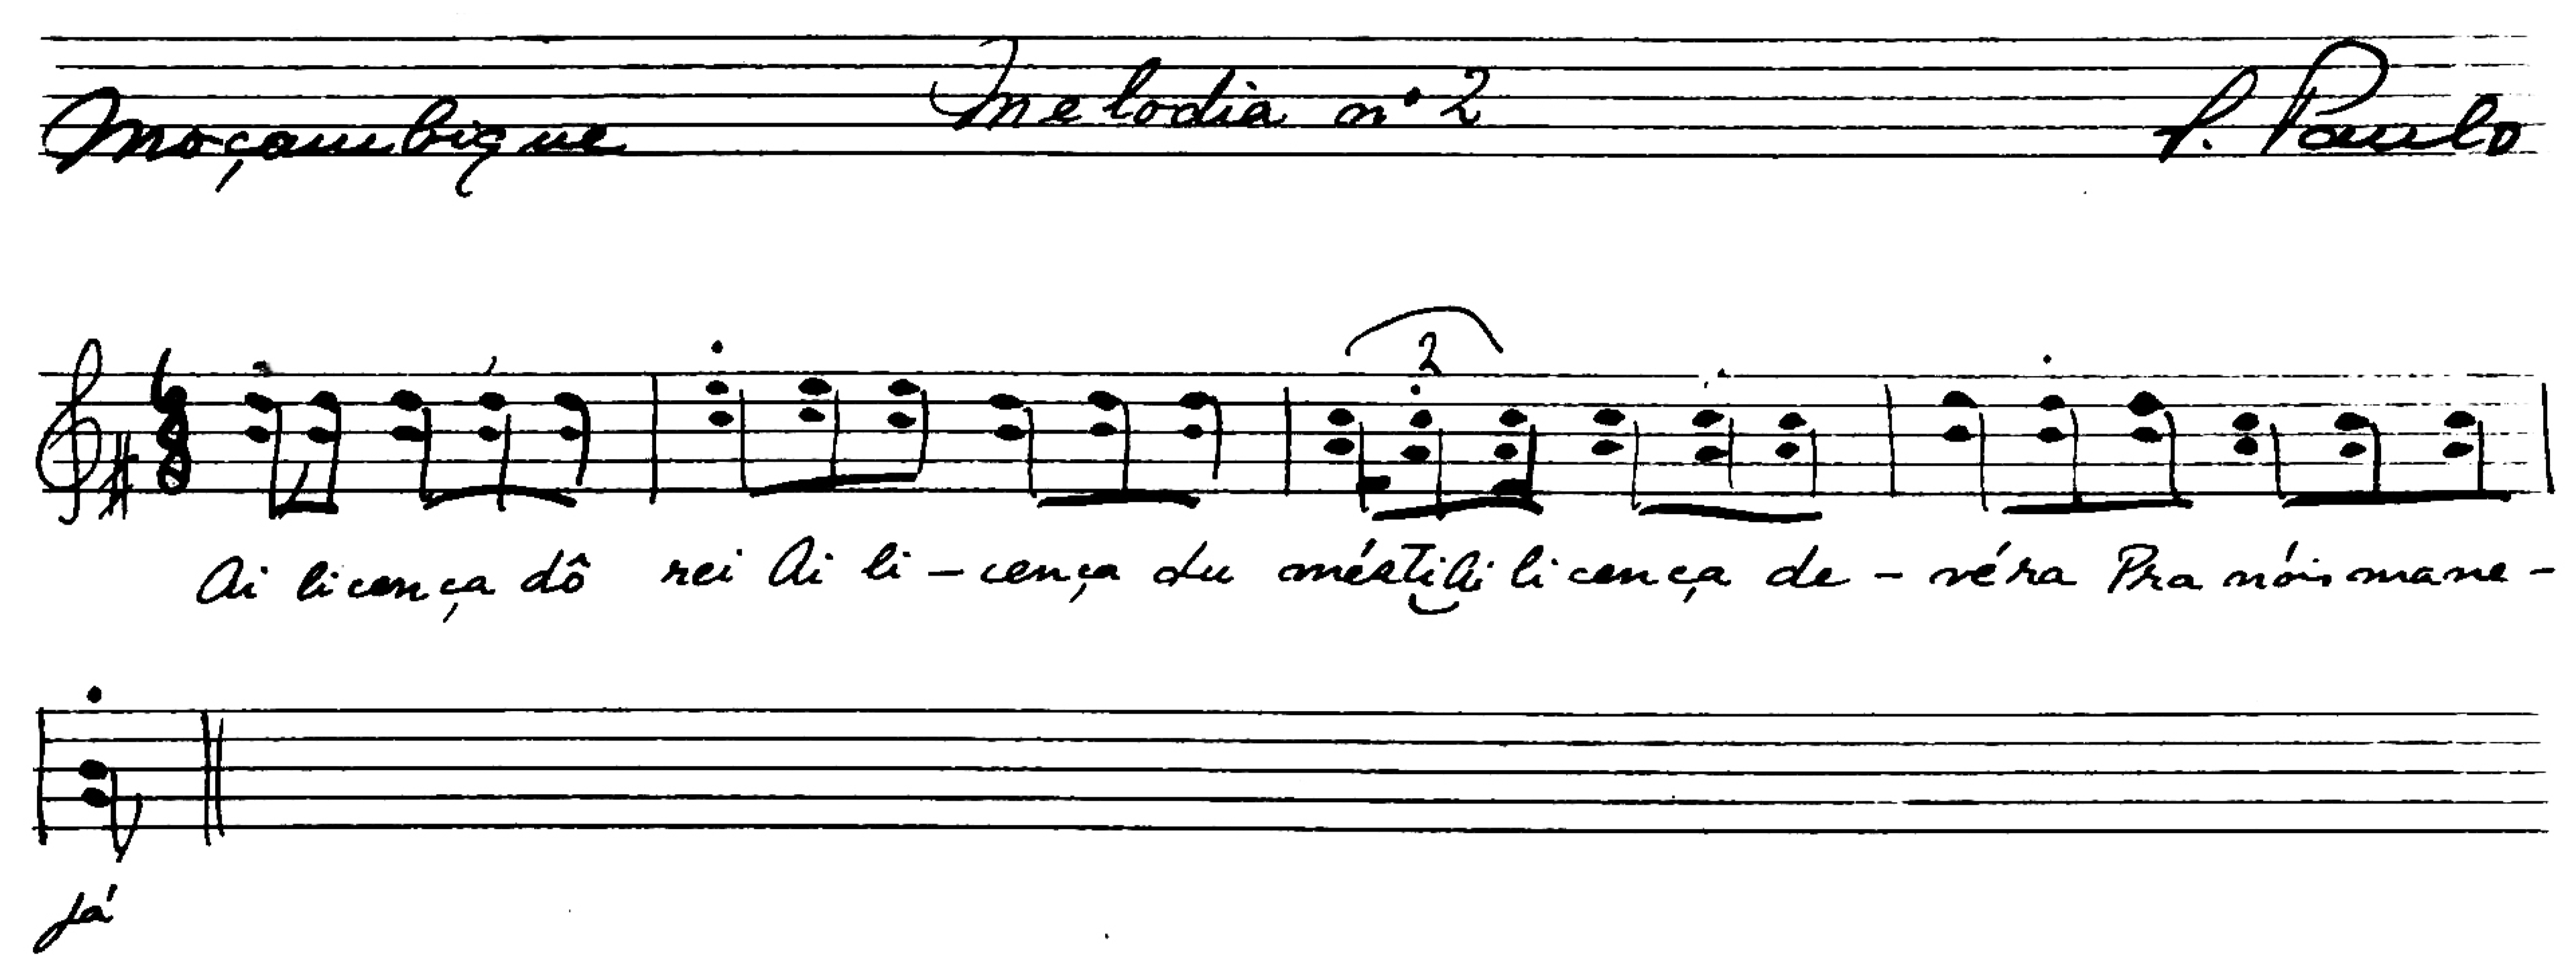
\includegraphics[width=100mm]{./imgs/img6.png}
%\caption{}
%\end{minipage}
\end{figure}

\begin{verse}
Ai, licença do Rei,\\
Ai, licença do Méstri,\\
Ai, licença devéra (deveras)\\
Pra nóis manejá!
\end{verse}
(A síncopa do terceiro compasso é mero fruto de dicção. A ligação da
sílaba ``tri'' de ``mestre'' com a interjeição ``Ai'' do verso seguinte,
formando um hiato, por assim dizer, oralmente muito pesado, obrigou a
conceder a esse hiato maior tempo ritmico.)

\section*{Figurações}

Aqui a coreografia se complicava muito, e as figurações ficaram dificeis
de descrever. 1: Usando sistematicamente a variante nº~2 do passo
tradicional, cada bailarino, segurando o bastão por uma extremidade,
estendia a outra extremidade pro bailarino fronteiro na outra fila, que
a segurava. Ficavam assim, cada dois bailarinos ligados entre si pelos
seus bastões e braços distendidos. Ao primeiro movimento de translação
prá frente, que os aproximava um do outro, cada qual erguia o braço
esquerdo ao passo que abaixava o direito, de forma a no início do
segundo tempo do compasso, os dois bastões estarem em posição vertical.
Ao segundo movimento de translação prá frente, cada bailarino dobrava
junto do peito, no cotovelo e no pulso, o braço esquerdo que se erguera
um pouco na traslação anterior, ao passo que o outro bailarino, que no
movimento anterior abaixara o seu braço direito correspondente a êsse
mesmo lado, o esticava de novo prá frente, como na intenção de abraçar o
companheiro, e fazendo, pois, o bastão passar por debaixo do sovaco
dêste. Como do outro lado, os dois bailarinos faziam o mesmo, só que em
sentido contrário, isto é, o que um faz do seu lado direito, o outro
fazendo tambem á sua direita, cada um dos dois fica abraçado duma banda
só, e com o bastão (que traz sempre seguro com a mão esquerda dobrada
junto do peito) lhe passando por debaixo do braço. Com as duas
translações pra trás, voltavam ao lugar do princípio, da mesma forma com
que desfaziam os gestos e ficavam na postura inicial. 2: Depois de
repetirem várias vezes essa figuração, unem os dois bastões na frente do
corpo e continuam repetindo o passo caracteristico na sua variante nº~3,
exclusivamente em translações laterais. Esta figuração se maneja de dois
em dois pares, cada par unido por dois bastões que ondulam na frente dos
corpos. Depois de repetirem várias vezes a coreografia nº~3, em
translações exclusivamente laterais, num momento dado, o primeiro par,
ao fazer o movimento de translação que o aproxima do par com o qual
perfaz a quadra, em vez dum simples passo ou pulinho, dá um grande pulo,
ao mesmo tempo erguendo os bastões unidos. O outro par da quadra, nesse
momento dá tambem um grande pulo, em sentido contrário, abaixando porêm
bastões e cabeças, de forma a passar por debaixo dos bastões unidos do
par com que dansa. Trocados, pois, os dois pares de lugar, os quatro
bailarinos giram rapido cada qual sobre si mesmo, sempre na direção da
esquerda prá direita. Mas os bastões perseveram unidos, segurados no
giro, primeiro só pela mão esquerda até que os dois bailarinos, que os
seguram, se darem as costas, e então segurados pela mão direita que foi
buscar os bastões ás costas, e os segura sozinha até que o corpo
completou o giro, e estão de novo os dois bailarinos se defrontando.
Recomeça outra vez a translação lateral ondulante, até que executam de
novo os dois pares o grande pulo, fazendo cada qual o que o outro fizera
no primeiro pulo, e voltando todos ás suas posições primitivas. 3:
Repete"-se a mesma figuração, mas de cócoras, em passo de one"-step. 4:
Todos erguidos, sempre na variante nº~3 do passo, em translação tambem
sempre lateral, e sempre de bastões unidos, mas seguros só com uma das
mãos, ou passando"-os duma para a outra mão, os bailarinos giram sobre si
mesmos, e depois, durante uma translação lateral, passam um dos pés (o
que executa primeiro o movimento de translação que está se realizando)
por cima dos bastões unidos.

\pagebreak

\section*{DANSA Nº~5}

\begin{figure}[!ht]
%\begin{minipage}{0,4\textwidth}
\centering
 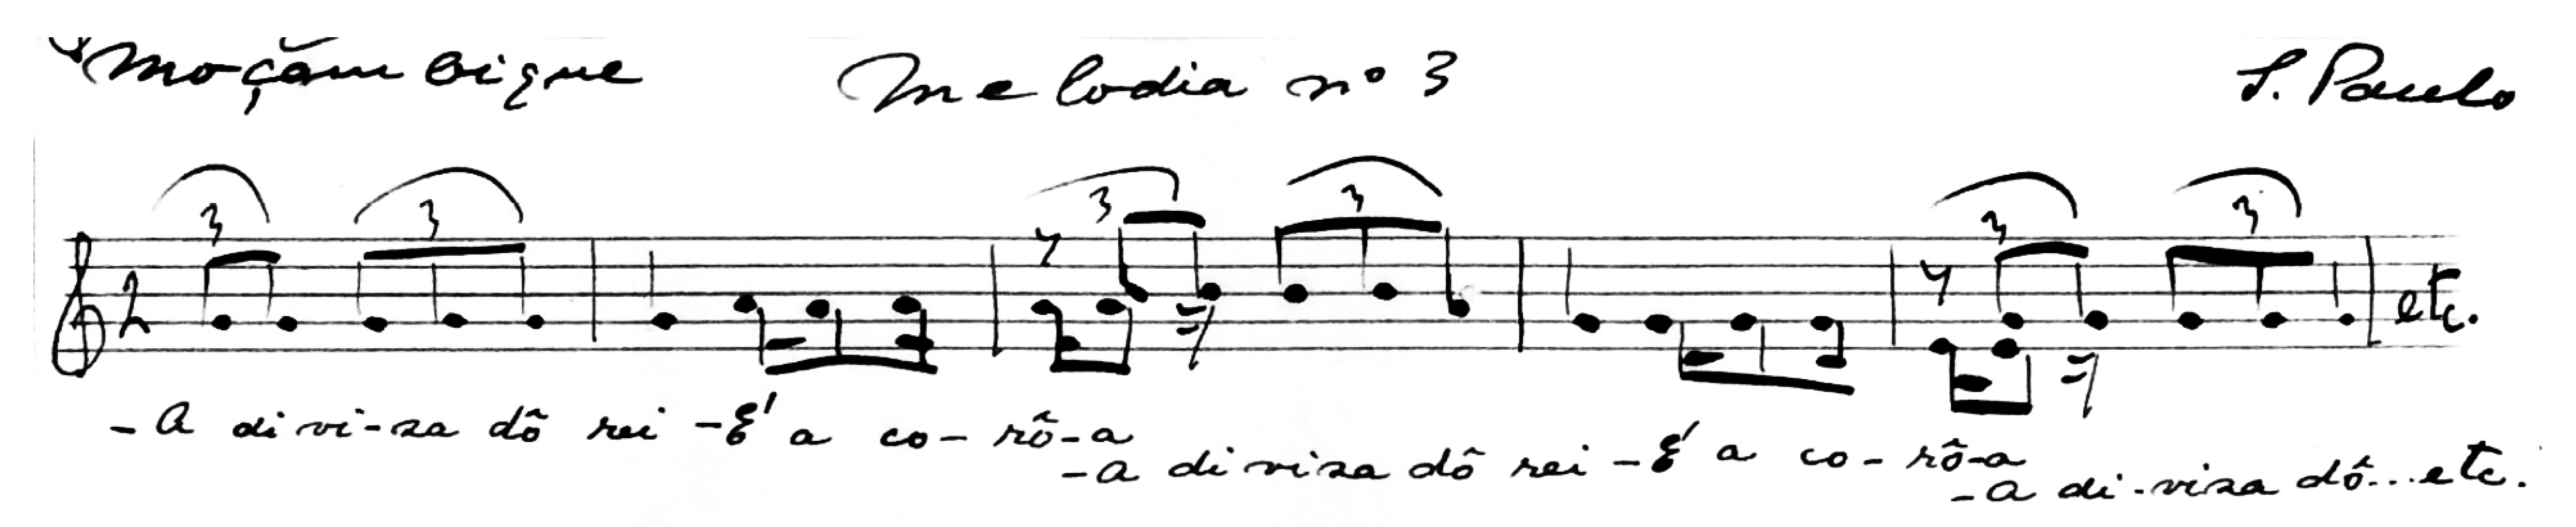
\includegraphics[width=100mm]{./imgs/img7.png}
%\caption{}
%\end{minipage}
\end{figure}

\begin{verse}
Solo: --- A divisa do Rei\ldots{}\\
Côro: --- É a corôa!
\end{verse}

\section*{Figurações}

Esta foi a unica, das dansas que vi, de que o Rei participou. Iniciada a
cantoria, o Rei foi se colocar no centro do bailado, entre as duas
fieiras, que já estão nos seus lugares, fazendo qualquer das variantes
do passo de tradição, em movimentos laterais. Quando o Rei para no
centro, imediatamente, sem perder o passo, os bailarinos formam roda
apertada em torno dele, e o cobrem com os bastões (que passaram prás
mãos direitas) e braços direitos distendidos. E nas mesmas translações
laterais de corpo, num vaivem gostoso, com traslações de passo pequenino
prá direita e de salto mais largo prá esquerda, giram lentamente,
ondulantemente, em volta do Rei. 2: O Rei se abaixa de sopetão. Todos o
imitam, e a roda continua girando de cócoras, em passo de one"-step.

\pagebreak

\section*{DANSA Nº~6}

\begin{figure}[!ht]
%\begin{minipage}{0,4\textwidth}
\centering
 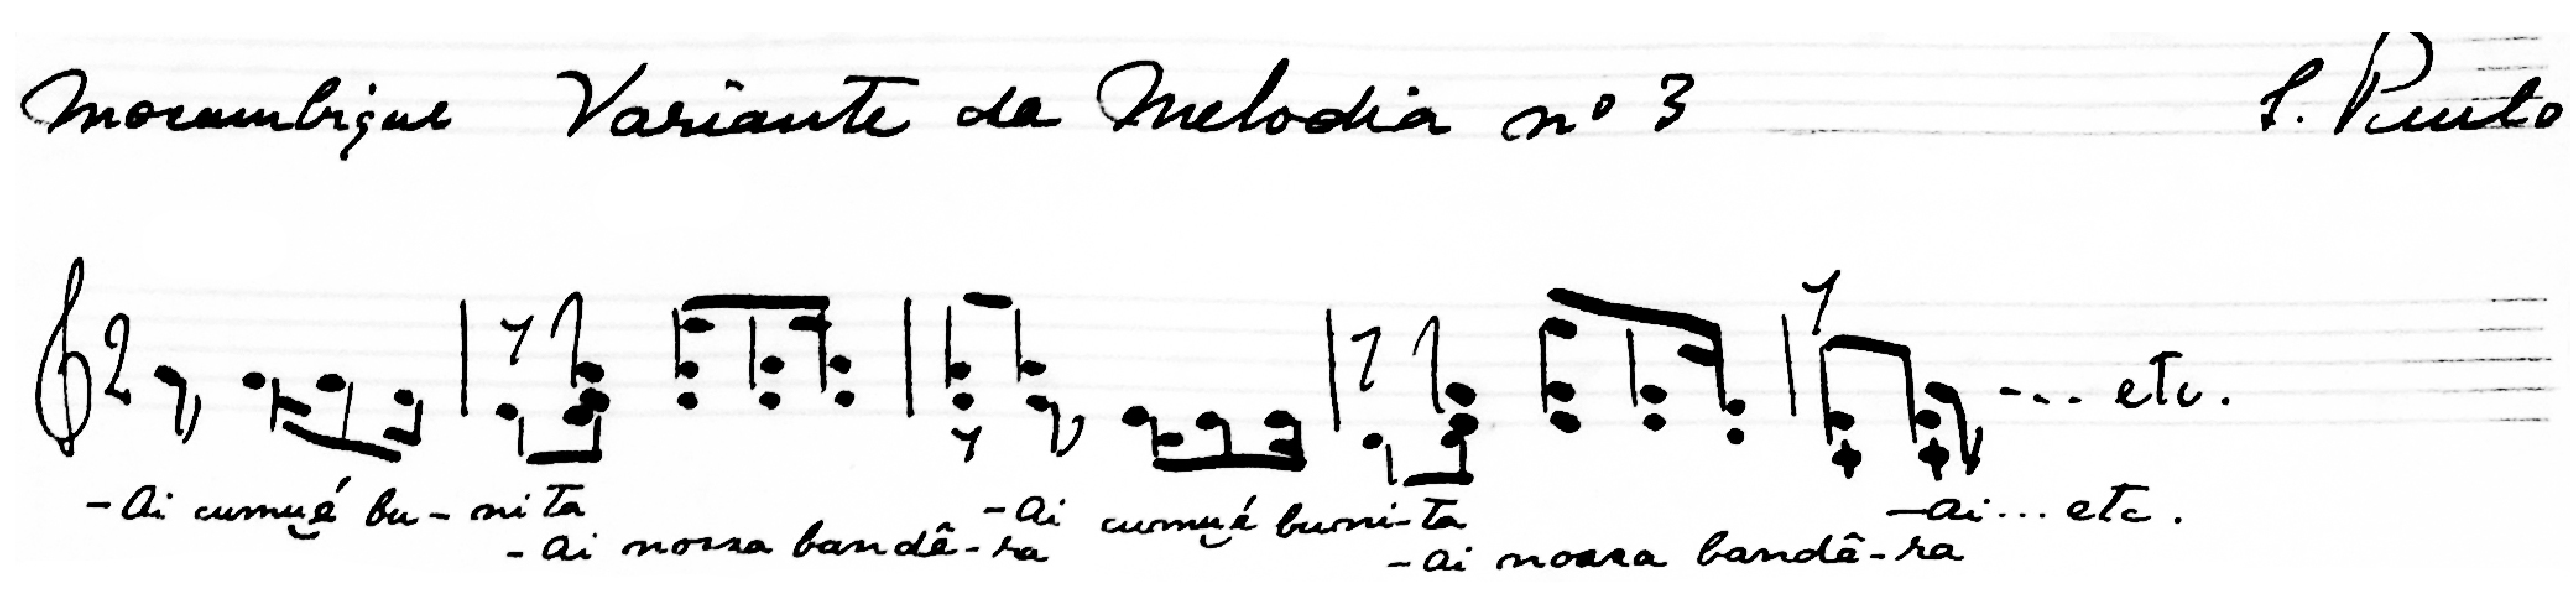
\includegraphics[width=100mm]{./imgs/img8.png}
%\caption{}
%\end{minipage}
\end{figure}

\begin{verse}
Solo: --- Ai, cumu é bunita\ldots{}\\
Côro: --- Ai, nossa bandêra!
\end{verse}

\section*{Figurações}

Este manejo funde de novo grupos de dois pares, e consiste numa
figuração apenas. No passo tradicional, em translações laterais, a um
momento dado, cada bailarino dá um pulo violento pra frente e atinge o
lugar em que estava o bailarino fronteiro na outra fila. Durante o pulo,
feito numa translação só, quando os dois bailarinos pulantes passam um
pelo outro, chocam violentamente os bastões. Chegado cada qual ao lugar
pra que se trasladou com o pulo, fazem todos meia"-volta rapida e repetem
tudo em sentido contrário, voltando cada qual ao seu lugar de início. Ai
chegado, cada bailarino faz esquerda ou direita volver, e repete tudo,
mas com seu par da mesma fileira.

\pagebreak

\section*{DANSA Nº~7}


\begin{figure}[!ht]
%\begin{minipage}{0,4\textwidth}
\centering
 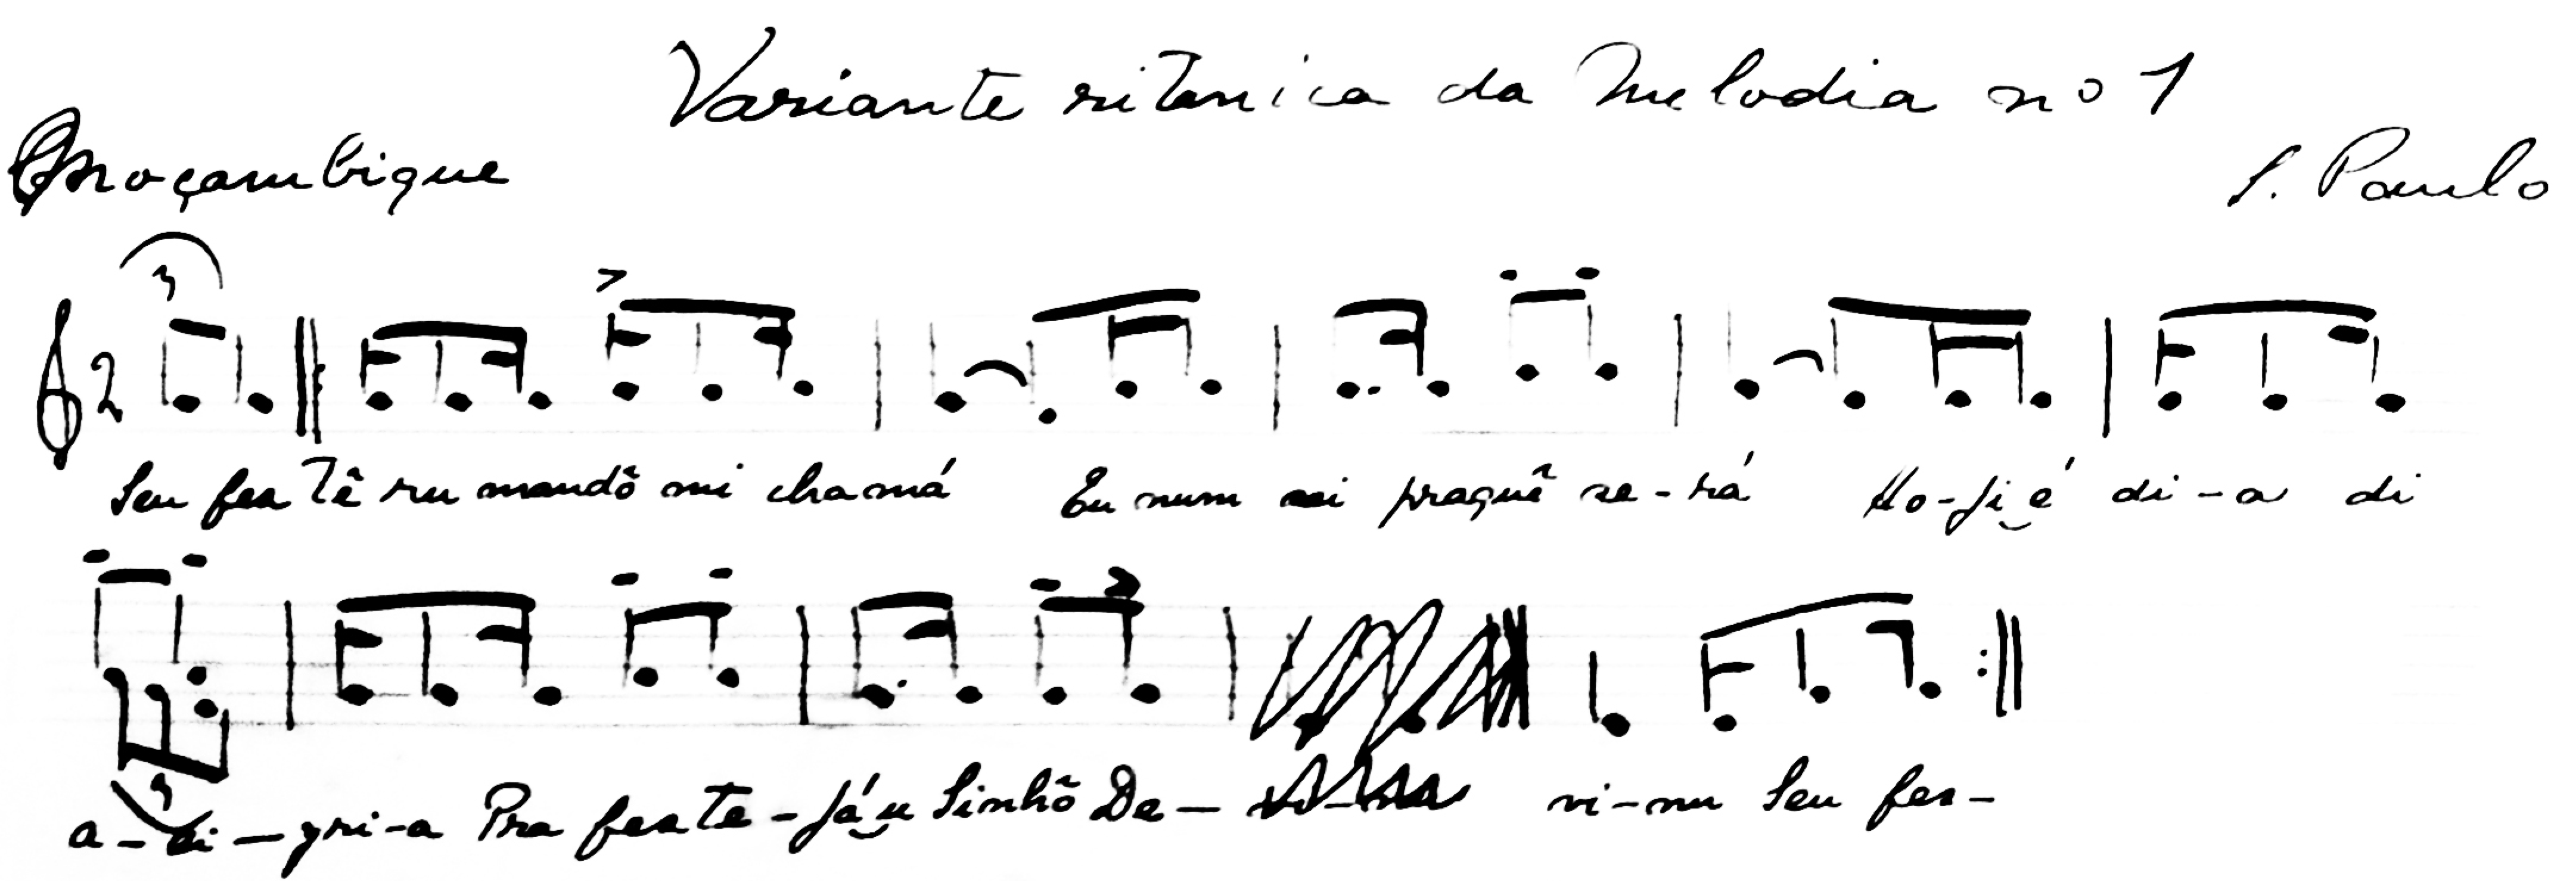
\includegraphics[width=100mm]{./imgs/img9.png}
%\caption{}
%\end{minipage}
\end{figure}

\begin{verse}
Seu festêru mandô mi chamá,\\
Eu num sei praquê será;\\
Hoji é dia di aligria\\
Pra festejá u Sinhô Devino!
\end{verse}

\section*{Figurações}

O manejo aqui é simples e funde de novo grupos de dois pares. O passo
agora é de one"-step e parece implicar a obrigação de não fazer nenhum
ruído com os conguinhos. Pelo menos os quatro primeiros bailarinos
pisavam com delicadeza visivelmente procurada, intencional, duma
verdadeira elegancia e vaporosidade coreografica. A posição de cada
bailarino consiste em trazer as duas mãos á cinta, mas a que traz o
bastão, e que deve ser a que fica do lado exterior de cada par da mesma
fila, se coloca de tal forma que o bastão fica empinado verticalmente
até a altura da cabeça do bailarino. Cada par está bem unido, os dois
bailarinos se encostando de ombro um no outro. Fixado o ritmo, a uma
entrada do solista, o manejo principia. Na arsis inicial da melodia, os
pés internos de cada par fazem um movimento de traslação prá frente, e
apoiam no chão ao início do primeiro tempo do primeiro compasso.
Imediatamente os pés externos do par, ficados atrás, se transladam num
passo inteiro prá frente dos outros pés, e vão se apoiar no chão ao
início do tempo seguinte. Com isso, cada par está agora de peito unido
com o par da outra fila, com o qual dansa. Imediatamente os pés internos
de cada par, ficados atrás, se transladam prá frente, não porêm em passo
inteiro, mas apenas em meio passo, vindo, pois, se colocar junto do pé
que está pousado. Agora, pois, como na postura inicial, o pêso do corpo
está aguentado pelos pés juntos. A unica habilidade coreografica
consistiu na leveza dos passos realizados, (sem nenhum remeleixo de
ancas) e na ``letra'' de, ao pousar junto do outro, o pé ficado atrás,
ergue"-lo uns vinte centimetros ou pouco mais do chão, dar a impressão de
que vai bater forte e soar os conguinhos, mas pousar levissimo, pisando
em ovos. Foram necessarios tres tempos pra se realizar todo êsse
movimento. O quarto tempo que completa a frase ritmico"-melodica, é
indicado por uma leve, bem leve curvatura de joelhos, dando ao corpo um
pequeno movimento ondulatorio de alto a baixo. Na arsis da segunda frase
da melodia, cada bailarino faz esquerda ou direita volver de forma a
emparelhar agora com o bailarino que defrontava, e o novo par ficar
unindo costas com o outro novo par da quadra. E, com os pés contrários,
perfazem, nos novos dois compassos, tudo quando fizeram nos dois
primeiros compassos da melodia, sempre em translações prá frente --- o
que faz os dois novos pares se afastarem um do outro. Na arsis da
terceira frase melodica, os quatro fazem meia"-volta, á esquerda ou á
direita, contanto que nêsse meio giro os dois bailarinos emparelhados se
dêm as costas. Tanto esta meia"-volta como o volver pro lado, não tomam
nenhum tempo ritmico, são executados durante a arsis inicial de cada
frase melodica, ao mesmo tempo que aquele dos dois pés pousados que
executa a primeira translação, se translada. A terceira frase melodica,
implicando os mesmos movimentos das duas frases anteriores, une de novo
os quatro bailarinos, peito a peito os pares. A quarta e última frase
enfim os separa de novo nos dois pares iniciais do manejo, e traz cada
bailarino ao seu lugar do início da dansa. Não porêm na mesma direção,
pois que tambem nesta frase melodica os movimentos de translação se
fazem prá frente, o que obriga, no final da frase, os pares que dansam
juntos estarem se dando as costas, e as duas fieiras não mais se
defrontando. Será pois necessaria nova meia"-volta pra reiniciar todo o
manejo, na repetição da melodia.

%\pagebreak

\section*{Conclusão}

Estas foram as figurações coreograficas, as melodias e observações que
pude anotar dêste bailado, visto em condições bastante precarias. As
melodias das dansas nº~1 e nº~4 foram registradas pelo compositor
Camargo Guarnieri. A melodia da dansa nº~5, a sua variante na dansa nº~6, bem como a pequena variante da primeira melodia que vem na dansa nº~7, foram anotadas por mim. É provavel que tenha, durante o dia e noite
que êsse Moçambique durou, surgido alguma nova linha melodica. Mas está
claro que numa excursão em que, por mais bem intencionados que fossemos,
predominava a liberdade do passeio e não a dedicação do estudo, com
horas determinadas pra almôço e pra volta a São Paulo, pela tardinha,
não era possivel uma colheita sistemática que esgotasse os valores
etnograficos do \emph{Moçambique}, de Santa Izabel. Embora êle fosse
pobre. Vi mais dansas que essas descritas, com as mesmas melodias e só
textos diferentes. Mas toda a vez que me propunha a registrar um texto,
eu carecia de me socorrer da Rainha, do Rei ou de mais alguem do
bailado, tal era, tão desmanchada e escura, a dicção do cantador e dos
bailarinos coristas. Alem disso, a pobreza intelectual dos textos
registrados, si não justifica a negligencia do recolhedor, parece
indicar uma possivel não tradicionalidade de muitos deles. A propria
coreografia, que era a parte mais interessante do bailado, se vê pelas
figurações descritas, que não formam manejos especificos e obrigatorios,
mas apenas outras tantas maneiras de mover o grupo, inventadas ad hoc,
pelo ensaiador do rancho; e que podem se combinar e desenvolver ao
infinito, com as figurações duma Quadrilha. Ressalvado algum possivel
engano, em que não creio mas que pode ter se dado nas condições
precarias do recolhedor, tomei bastante cuidado no descrever
pormenorizadamente os manejos que vão aqui. Isso porquê me pareceu que
no \emph{Moçambique}, pobre de texto e de música, se dava um cuidado
muito particular em desenvolver o manejo coreografico. E com efeito,
pelo que já tenho observado de dansas"-dramaticas brasileiras, estou que,
como coreografia, não êstes dansarinos, mas êste bailado de Santa
Izabel, é mais desenvolvido e mais rico que as dansas"-dramaticas
nordestinas. No Nordeste encontrei bailarinos de admiravel virtuosidade
pessoal, não porêm tamanha variedade e pesquisa de figurações
coreograficas, a não ser nos \emph{Cabocolinhos}. E mesmo êstes não
possuíam um passo especifico, enquanto o Moçambique apresenta um passo
caracteristico, de grande originalidade, que jamais não vi descrito. É o
que vale mais, de tudo o que recolhi.

E quando, terminadas as dansas numa casa, o rancho vai pelas ruas, vai
sem dansa, em passo humano, mas usando como dobrado de marcha, a
variante melodica que está na dansa nº~6. Com o texto seguinte:

\begin{verse}
Solo: --- A bandêra na rua\ldots{}\\
Côro: --- É siná di guerra!\\[5pt]
\end{verse}

\noindent{}O que será provavelmente reminiscencia dos Congados\ldots{}

\bigskip
\begin{flushright}
Mario de Andrade

São Paulo, Junho"-de 1933
\end{flushright}

\part{\textsc{ensaios}}

\chapter*{Mário de Andrade, Moçambique\\ e a Santa Cruz}
\addcontentsline{toc}{chapter}{Mário de Andrade, Moçambique e a Santa Cruz, \emph{por Enrique Menezes}}
\hedramarkboth{Mário de Andrade, Moçambique\ldots{}}{}

\begin{flushright}
\textsc{enrique menezes}
\end{flushright}

Nos idos da década de 1840, um alemão chamado Carl Philipp von Martius
advertia que quem quisesse escrever sobre a história do Brasil deveria
considerar ``elementos de natureza muito diversa, tendo para a formação
do homem convergido de um modo particular três raças, a saber: a de cor
de cobre ou americana, a branca ou caucasiana, e enfim a preta ou
etiópica''.\footnote{Martius, Karl Friedrich Philipp. \emph{Como se deve
  escrever a História do Brasil}.} Desde então, a lista de intérpretes
do Brasil que de alguma forma se referiram a essa narrativa de
``formação'' de um ``homem'' brasileiro vai longe, e poderíamos lembrar
alguns desses \emph{homens}: Capistrano de Abreu, Paulo Prado, Cornélio
Pires, Sérgio Buarque de Holanda, Gilberto Freyre, Silvio Romero, entre
tantos outros. Essa instrução também fez a cabeça de muito teórico da
música brasileira, gerando uma série de interpretações, explicações e
teorias da formação que se construíram sobre o famoso mito das três
raças. O musicólogo Vasco Mariz coloca de maneira clara na abertura de
sua \emph{História da Música no Brasil}: ``três raças que concorreram
para a eclosão do tipo brasileiro: a branca, a negra e a
vermelha''\footnote{Mariz, Vasco. \emph{História da música no Brasil},
  pg. 25.}.

Também havia feito a cabeça do poeta Olavo Bilac, que cantava em versos
--- hoje famosos --- a versão desse ``mito originário'' na música
nacional, ecoando um choro canônico, como a ``flor amorosa de três raças
tristes''\footnote{No poema ``Música brasileira'', publicada no livro
  \emph{Tarde} {[}1919{]}.}. O poeta canta nossa música como o encontro
requebrado e impuro de ``bárbara poracé'', ``banzo africano'' e
``soluços de trova portuguesa'', resultado ``cujos acordes são desejos e
orfandades de selvagens, cativos e marujos'', uma ``lasciva dor, beijo
de três saudades''. O folclorista Luís da Câmara Cascudo também
caprichou numa versão dessa narrativa:

\begin{quote}
a população de portugueses, índios e negros no Brasil foi marcada pela
melancolia e tristeza decorrentes do afastamento de seu lugar de origem,
contribuindo sobremaneira para a formação de uma música folclórica
nacional. (\ldots{}) Cada um devia cantar as canções de seu país. De todas
elas amalgamadas e fundidas em um só molde --- a língua portuguesa, a
língua do vencedor --- é que se formaram nos séculos seguintes os nossos
cantos populares.\footnote{Cascudo, L. C. in Romero, S. ``Prefácio'' in
  \emph{Folclore Brasileiro: Cantos Populares do Brasil}.}
\end{quote}

É também como Cornélio Pires via a coisa, e em 1929 narrava em disco
comercial uma versão caipira"-paulista do mito para introduzir a ``moda
do peão'' nas vozes da dupla Mariano e Caçula:

\begin{quote}
Moda de viola cantada por dois genuínos caipiras paulistas. Este é o
canto popular do caipira paulista em que se percebe bem a tristeza do
índio escravizado, a melancolia profunda do africano no cativeiro e a
saudade enorme do português, saudoso da sua pátria distante. Criado,
formado nesse meio nosso caipira, a sua música é sempre dolente, é
sempre melancólica, é sempre terna. Eis a moda do peão.\footnote{Mariano
  e Caçula, ``Moda do Pião'' {[}1929{]}.}
\end{quote}

Em um texto datilografado (não assinado) que está no arquivo pessoal de
Mário de Andrade, escrito em 1938 provavelmente pelo prefeito de Atibaia
na época, João Batista Conti (com quem Mário trocava cartas e
informações)\footnote{Conferir Valentini, Luísa. \emph{Um laboratório de
  antropologia: o encontro entre Mário de Andrade, Dina Dreyfus e Claude
  Lévi"-Strauss: 1935--1938}.}, chamado ``As congadas de Atibaia'',
podemos ler a resposta de um mestre congadeiro, Caetano Avelino da
Silveira, o ``mestre Caetano'', de 87 anos, natural de Atibaia e filho
de africanos, à pergunta feita pelo prefeito sobre a origem das
congadas. A resposta transcrita é outra interessante versão paulista da
narrativa:

\begin{quote}
Diziam os antigos, e é por conta deles porque eu não vi, que quando
nasceu o menino Jesus na Terra Santa, havia treis reis: um branco, um
preto e um caboclo. Os reis branco, querendo lográ o preto disserum que
para ver o menino Jesus era perciso dá uma volta muito grande e
ensinaram um caminho errado, pro preto ficar logrado. E assim forum os
treis vê o Senhor Menino. Mais o preto pegô o caminho errado. Quando os
branco chegaram na cocheira onde tava o Menino Jesuis derum com o preto
já na frente do menino Jesuis, que entonces o Senhor menino pegô uma
coroa, pois na cabeça do reis preto e disse: `Vassuncê é o dos Congos'.
Foi entonces que o preto foi chamá uma porção de negros e vierum dançá
na frente do Menino, daí, em diante ficô a congada. E é por isso que os
reis da Congada leva a coroa na cabeça, branco num pode.\footnote{``As
  congadas de Atibaia'', Arquivo Mário de Andrade, \versal{IEB-USP}.}
\end{quote}

Mário de Andrade é mais um dos muitos \emph{homens} que compraram a
prazo essa narrativa --- ainda hoje bastante presente --- e que aparece em
diversos momentos da sua criação e reflexão. Em 1928 marcava seu
clássico \emph{Macunaíma}, aparecendo também, no mesmo ano, no seu
\emph{Ensaio sobre a música brasileira,} aí com uma medida: ``a
ameríndia em porcentagem pequena; a africana em porcentagem bem maior; a
portuguesa em porcentagem vasta''\footnote{Andrade, Mário de.
  \emph{Ensaio sobre música brasileira}, {[}1928{]} pg. 20.}. Uma visita
ao arquivo pessoal do escritor revela, em um sem"-fim de pequenas
anotações, que ele perseguiu durante toda a vida essa espécie de
proporcionalidade de influências entre o que ele chama de três
diferentes ``raças''.

Os dois textos de Mário de Andrade aqui revisitados e
republicados\footnote{Esses textos foram editados por Oneyda Alvarenga e
  publicados em \emph{Danças dramáticas do Brasil 3º tomo} (Itatiaia,
  1982) e \emph{As melodias do boi e outras peças} (Duas Cidades, 1987).}
são interessantes para se observar as maneiras pelas quais o escritor
pensa a narrativa das três raças de um modo específico, a começar pelo
fato de se tratar de registros feitos no interior do estado de São
Paulo. O estudo das manifestações culturais paulistas segue uma pulsação
de trajetos que era comum para a população paulistana. O movimento em
direção a celebrações religiosas que envolviam atos dramáticos, festas,
danças e outras modalidades de performance se motivava tanto pela
devoção quanto pela beleza e pela convivência familiar e pública que
proporcionavam. E é no que se chamavam, à época, os arredores de São
Paulo, e nos territórios onde a estagnação econômica deixava à mostra as
marcas da ainda recente explosão cafeeira e da mobilização da
mão"-de"-obra escravizada, que os interessados na contribuição histórica
de indígenas e africanos encontravam as paisagens que lhes pareciam mais
reveladoras\footnote{Ver Valentini, Luísa. ``Nos `arredores' e na
  `capital': as pesquisas da Sociedade de Etnografia e Folclore
  (1937--1939)''.}. Esses dois textos de Mário deixam claro que esse
sentido de revelação tem, para esta geração, o sentido de uma viagem no
tempo (no fim da vida o escritor lembra seus ``passeios constantes ao
passado paulista, Sorocaba, Parnaíba, Itú\ldots{}''\footnote{Andrade, Mário
  de. ``O movimento modernista'', \emph{Aspectos da Literatura
  brasileira}, p. 241.}) --- efeito então muito disseminado, e que só
começa a sofrer uma crítica sistemática a partir de meados do século \versal{XX}.
O sentimento específico que acompanha esse modo de pensar as marcas
históricas numa paisagem cuja transformação --- e esquecimento --- parece
iminente, é esmiuçado em melancólica ironia pelo próprio Mário no texto
sobre a dança de Santa Cruz, na qual ele reconhece ``um rescaldo tão
vivo ainda de indiada (\ldots{}) chegava a assombrar''.

Em nossos dias, as presenças negras e indígenas em São Paulo se
reivindicam, se manifestam e se fazem reconhecer como vivas e ativas (em
vez de ``rescaldos''), o que faz com que soe estranha a ideia de
``sobrevivência'' por meio da qual já se pensou essas manifestações.
Hoje se reconhece o quanto é ofensivo tratar como mortas ou quase"-mortas
as expressões mantidas belas e ativas por tantas gerações cantantes,
dançantes, louvantes e brincantes. Sempre vale lembrar que ideias
frequentemente enunciadas por Mário, como a de ``perda'' e a de
``empobrecimento'', cuja figuração evoca por contraste um passado cheio
e idealizado, nos dizem de um contexto em que projetos violentos como os
de embranquecimento e até de eugenia eram
correntes e abertos, atravessando e orientando as ciências, o Estado e a
educação.\footnote{Isso certamente tem algo a nos ensinar, especialmente
  num momento em que os próprios praticantes de manifestações
  tradicionais reativam as ideias de perda e desaparecimento para falar
  dos riscos e agressões cotidianamente enfrentados, e que são motivados
  por paradigmas cujos efeitos destrutivos eles conhecem bem.}

Hoje nosso escritor teria acesso a dados muito mais precisos, e levaria
um susto enorme ao acessar a base de dados colaborativa internacional
\emph{slavevoyages.org} e descobrir que, até o final do processo
colonial, teriam desembarcado no Brasil algo em torno de 4,8 milhões de
africanos, cerca de sete vezes mais do que os 750 mil portugueses que
ficaram por aqui. Estima"-se ainda, no século \versal{XVI}, a presença de 2,43
milhões de índios no que é hoje o território brasileiro, número que,
como se sabe, foi diminuindo brutalmente ao longo do tempo.\footnote{Esses
  números foram reunidos por Alencastro no texto ``África: números do
  tráfico atlântico'', baseado no Slave Trade Database (para africanos
  desembarcados no Brasil), em John Hemming (para indígenas, no livro
  \emph{The red gold}) e em suas próprias pesquisas para portugueses. Em
  Schwarcz, Lilia e Gomes, Flávio dos Santos (Orgs.). \emph{Dicionário
  da escravidão e liberdade: 50 textos críticos}, 2018. É claro que
  precisamos considerar que a mortalidade indígena aumenta muito,
  enquanto o número de africanos desembarcados cresce durante todo o
  período colonial, e o de imigrantes europeus cresce muito após a
  extinção do tráfico de africanos.} Além disso, entre os africanos
chegados, aproximadamente três quartos deles (3,6 milhões) haviam saído
de portos na África central. Nos portos do sudeste em particular, os
africanos centrais desembarcados chegam a mais de 95\%.

E é mesmo para a direção dos dados atuais que apontam esses textos de
Mário. Ao visitar festas populares, o escritor nota alguma presença
indígena na dança de Santa Cruz, em Carapicuíba, e muita presença negra
no moçambique (de Santa Isabel e Mogi das Cruzes), na congada (de Mogi,
Lindóia, Atibaia e Lambari), no samba rural, no choro urbano, na
``música de feitiçaria'', entre outros. Se olharmos para seu conjunto de
textos sobre música popular brasileira em geral, encontraremos muita
tinta sobre características que o escritor suspeita derivarem da
presença cultural africana no Brasil, o que leva o musicólogo Tiago de
Oliveira Pinto a anotar uma importante diferença entre a abordagem de
Mário e a de pesquisadores alemães que no início do século \versal{XX} visitavam
o Brasil curiosos em relação à ``música autêntica'' do país:

\begin{quote}
Mário de Andrade não conseguia entender por que os musicólogos alemães
consideravam a música indígena como ``autêntica música brasileira''. Em
carta de 22 de junho de 1928, faz a seguinte proposta a {[}Marius{]}
Schneider: ``Lamento não poder fornecer mais do que algumas informações
incompletas sobre a bibliografia musical dos índios do Brasil. Meu campo
de pesquisa é bastante diferente, é limitado ao folclore e incluo uma
monografia em que considero a influência dos negros da África no samba
afro"-brasileiro''.\footnote{Oliveira Pinto e Ribeiro. ``The ideia of
  modernismo brasileiro''. A carta de Mário é, na verdade, de 1938,
  visto que o texto ``Samba Rural Paulista'' é de 1937.}
\end{quote}

A monografia anexada à carta era o texto ``Samba Rural Paulista'', no
qual o escritor elenca diversos pontos de contato entre o samba rural de
São Paulo e práticas africanas que ele conhece em livros de, entre
outros, Eric V. Hornbostel, Natalie C. Burlin, André Gide, Arthur Ramos,
Manoel Quirino, Maud C. Hare e Stephen Chauvet. Ainda que muitos textos
de Mário tenham formulações datadas e ``construções unanimistas'' de
África (uma ``falácia metonímica'' bastante frequente na qual a parte
{[}uma região ou característica{]} passa a representar a totalidade {[}a
``África''{]}\footnote{Prática criticada, entre outros, pelo filósofo
  Paulin Hountondji e mencionada pelo musicólogo Kofi Agawu em \emph{The
  african imagination on music}.}), o trecho ilumina o pesquisador
interessado que, marcando uma diferença em relação à inclinação
``indianista'' dos pesquisadores alemães, começa a perceber que a
história cultural africana é um forte fundamento da música brasileira ---
e americana em geral. Em uma análise sobre as relações entre práticas
musicais brasileiras e africanas, Oliveira Pinto afirma de modo
categórico:

\begin{quote}
Mário de Andrade (\ldots{}) foi pioneiro no entendimento da importância da
história cultural africana no Brasil e na América através de suas
expressões musicais.\footnote{Oliveira Pinto, Tiago de. ``Crossed
  Rhythms: African Structures, Brazilian Practices, and Afro"-Brazilian
  Meanings'' p. 167.}
\end{quote}

Esse pioneirismo em relação à presença negra nas expressões musicais
brasileiras impressiona se tivermos em mente que o ambiente no qual
Mário buscava se inserir era dominado por ricaços que cultivavam
abertamente ideias racistas, de supremacia branca e estratégias de
embranquecimento da população. Leia"-se como exemplo o editorial do
jornal \emph{O Estado de São Paulo}, assinado por Júlio de Mesquita
Filho, a 15 de Novembro de 1925, aniversário da proclamação da
república:

\begin{quote}
Promulgado o decreto de 13 de maio, entrou a circular no sistema
arterial do nosso organismo político a massa impura e formidável de 2
milhões de negros, subitamente investidos das prerrogativas
constitucionais. A esse afluxo repentino de toxinas, provocado pela
subversão total do metabolismo político e econômico do país, haveria
necessariamente de suceder grande transformação na consciência nacional
que, de alerta e cheia de ardor cívico, passou a apresentar, quase sem
transição, os mais alarmantes sintomas de decadência moral.\footnote{``A
  crise nacional'', O Estado de São Paulo, 15/11/1925.}
\end{quote}

O mau gosto das formulações racistas em metáforas médicas e biológicas
--- já nem pasmamos mais --- são do dono de um influente jornal que, junto
à elite intelectual paulista, fundaria a Universidade de São Paulo.
Ainda que circulasse nesse meio, Mário de Andrade encontrava mais
interlocução no pensamento de intelectuais como, entre outros, Arthur
Ramos e Roger Bastide, que partilhavam o interesse pela história
cultural africana no Brasil. Bastide, ao enviar para Mário um exemplar
do livro de sua autoria, \emph{Éléments de sociologie religieuse},
escreve em dedicatória: ``Ao grande romancista e africanista brasileiro
Mário de Andrade''\footnote{A relação de Mário com os estudos
  africanistas, a partir dessa dedicatória, é analisada por Ligia
  Fonseca Ferreira em ``Mário de Andrade, africanista'', em Andrade,
  Mário, \emph{Aspectos do folclore brasileiro}.}. O professor francês
reconhecia assim o esforço do escritor brasileiro em contribuir para o
debate sobre as presenças africanas nas Américas, que crescia também no
Brasil durante as décadas de 1920/30.

Caberia supor que Mário de Andrade tenha tido essa sensibilidade por ter
ele mesmo ascendência negra? Oswald de Andrade, ao conhecê"-lo ainda como
estudante do Conservatório Dramático Musical, descreve"-o como ``um aluno
alto, mulato, de dentuça aberta e de óculos''\footnote{Andrade, Oswald
  de. \emph{Um Homem sem profissão}, p.105.}, e seu biógrafo Eduardo
Jardim esclarece que ``seus traços mulatos tinham a ver com as duas
avós, Ana Francisca, do lado materno, e Manoela Augusta, do
paterno''.\footnote{Jardim, Eduardo. \emph{Eu sou trezentos: vida e
  obra.}} O próprio escritor afirma ter sido alvo do ``possível insulto
(\ldots{}) --- Negro!'', atrelado ao que chamou de uma ``cor duvidosa'',
embora, em um poema\footnote{Transcrito também em Camargo, Oswaldo de.
  \emph{Negro Drama Ao Redor da Cor Duvidosa de Mário de Andrade}.},
afirmasse:

\begin{verse}
De certo que essas cores também tecem minha \qb{}roupa arlequinal,\\
Mas eu não me sinto negro, mas eu não me \qb{}sinto vermelho,\\
Me sinto só branco, (\ldots{}) só branco em minha \qb{}alma crivada de raças!
\end{verse}

Dado o contexto no qual Mário circulava, Oswald caprichava no
\emph{bullying} caso realmente tenha feito circular um artigo no qual
chama o amigo de ``boneca de piche'', unindo aqueles que se tornariam os
principais tabus de sua biografia\footnote{``Dizem que há um artigo de
  Oswald, terrível, chamado Boneca de Piche, em que ele diz que no Mário
  de Andrade conviviam um mulato, um padre, um hipócrita, uma coisa
  assim, não me lembro bem como é, mas era uma coisa altamente ofensiva,
  e que isto foi lido pelo Mário à saída de um jantar que ele tivera com
  o Oswald. Mas essas coisas eu jamais consegui apurar.'' Depoimento de
  Mário da Silva Brito em Lopez, Telê Porto Ancona (Org.). \emph{Eu sou
  trezentos, eu sou trezentos e cincoenta: Mário de Andrade visto pelos
  seus contemporâneos}, p. 121--132.}. Nunca mais retomariam a amizade.
Não que a ascendência negra fosse o motivo da briga pois, ainda amigos,
brincavam com isso em viagem a Minas Gerais. Como levantou seu biógrafo,
o grupo de amigos modernistas registrava assim seus nomes no Hotel
Macedo, em São João Del Rei:

\begin{quote}
Dona Olívia Guedes Penteado, solteira, photographer, anglaise, London.
Dona Tarsila do Amaral, solteira, dentista, americana, Chicago. Dr. René
Thiollier, casado, pianista, russo, Rio. Blaise Cendrars, solteiro,
violinista, allemand, Berlin. Mário de Andrade, solteiro, fazendeiro,
negro, Bahia. Oswald de Andrade Filho, solteiro, escrittore, suisso,
Berne. Oswald de Andrade, viúvo, escolar, hollandez, Rotterdam.
\end{quote}

A hipótese biográfica talvez possa contribuir para a possibilidade de
que Mário pudesse sentir na pele a desqualificação da ideologia corrente
no meio paulista, que entendia o negro como uma raça diferente da
euro"-americana (e pior)\footnote{Ligia Fonseca Ferreira, no artigo
  citado, acredita que a ascendência negra está entre as razões do
  escritor para ter se inserido em uma rede de estudos africanistas. Cf.
  ``Mário de Andrade, africanista'', p. 198.}. Em seus últimos dias como
diretor do Departamento de Cultura de São Paulo, antes de ser demitido,
Mário prepara uma conferência para o Cinquentenário da Abolição da
Escravatura, realizado em 1938. Baseada em outros textos e estudos seus
(em particular ``A superstição da cor preta'' e ``Linha de cor''), o
escritor afirma na conferência que o preconceito contra o negro derivava
de uma ``superstição primária e analfabeta de que a cor branca simboliza
o Bem e a negra simboliza o Mal (\ldots{}) se o branco renega o negro e o
insulta, é por simples e primária superstição.''\footnote{Andrade, Mário
  de. ``Cinquentenário da abolição'', em \emph{Aspectos do folclore
  brasileiro}.} Embora o próprio escritor recaia por vezes em uma
ideologia racialista, seus textos sobre racismo e ``superstição da cor
preta'' apontam, por outro lado, para uma diferenciação que não é
``natural'', (``não se trata de uma questão antropológica, nem da
estupidez de um Gobineau ou de um ariano''\footnote{Idem.}) mas
cultural, o que implica também uma outra perspectiva para a musicologia.

Bem dimensionado o grande número de
africanos chegados no Brasil durante o período escravista e sua
participação na música brasileira, talvez possamos identificar --- na
medida das nossas possibilidades --- esse nexo nos textos de Mário, visto
que em seu entendimento das danças paulistas, canto, movimento e devoção
não estão separados, mas são imediatamente conectados no corpo
dançante/musical/enfeitado/devoto (nexo que também pode ressoar em
tradições indígenas). A tentativa de desmembrar os termos acabaria com a
festa. Nesse sentido, sua abordagem se sofistica ao direcionar uma
apreciação que considera contextos maiores e suas diversas dimensões,
onde o musical é também imediatamente gestual, corpóreo, religioso e
pedagógico, entre tantas coisas. No moçambique, o nome do ``gênero
musical'' é também a dança e a nação diaspórica; a festa reforça
fundamentos comunitários, incorporativos, que coordenam e afirmam a
união, um caminho diverso daquele europeu, individualizado,
virtuosístico e autoral.\footnote{Características da imaginação
  africana, entre outros, em Kofi Agawu e diferenças entre concepções
  europeias e africanas de indivíduo e grupo em Joseph Miller,
  ``Restauração, reinvenção e recordação: recuperando identidades sob a
  escravização na África e face à escravidão no Brasil''.}
Oliveira Pinto chama a atenção, ainda, que para Mário de Andrade

\begin{quote}
o estudo musicológico só poderia ser entendido adequadamente em conexão
com outros domínios culturais, como a linguagem, a literatura, jogos e
peças dramáticas, arte visual e o contexto sociocultural em constante
mudança no Novo Mundo.\footnote{Oliveira Pinto, Tiago de. ``Crossed
  Rhythms: African Structures, Brazilian Practices, and Afro"-Brazilian
  Meanings'', p. 167.}
\end{quote}

A contribuição dessa perspectiva é valiosa por incorporar, de modo
orgânico à música, sua conexão com os outros domínios culturais ---
nesses textos sobre música paulista em especial, a conexão com a dança,
o movimento, o corpo --- se aproximando de modo mais apropriado à
realidade das manifestações musicais brasileiras. Nelas, a narrativa
musical está muitas vezes multiplicada pelo espaço gestual e pela
dimensão festiva. Mário cria assim uma outra camada de compreensão, que
se afasta do caminho euro"-cristão de uma ``música absoluta'' (que
privilegia a audição e tende a separar a música de sua relação com o
corpo).

Essa perspectiva guarda em si longo desenvolvimento: a possibilidade de
projetar a expressão musical pelo prisma do corpo. No caso das presenças
negras no Brasil, um corpo situado historicamente: na travessia forçada
através do Atlântico o africano escravizado não podia levar nada consigo
a não ser seu próprio corpo. Daí que esse corpo seja uma espécie de
objetivo e limite mesmo do escravismo no Brasil: frente à arbitrariedade
da escravidão e à tendência à dispersão de vínculos que acarreta, o
corpo forçado ao trabalho carrega também a continuidade impossível de
ser apagada: a expressão cultural através de uma certa qualidade de
movimentos, ideias e, para o pesadelo do senhor de escravos, a
possibilidade de revolta e fuga. Esses movimentos, ideias e
possibilidades vão ser expressos e re"-equacionados na realidade possível
do ``novo mundo''.

Os próprios termos portugueses ``música'' e ``dança'' podem, de certo
modo, ser relativizados se entendidos do ponto de vista das
manifestações culturais brasileiras e sua episteme negra, visto que
grande parte das línguas africanas tradicionais não têm uma palavra que
corresponda suficientemente a ``música'' e ``dança'', no modo europeu de
entendê"-las. De uma perspectiva africana, os termos seriam
``especializados'' demais. Kofi Agawu lembra, como exemplo, que ``entre
os tswana e os botswana, cantar e dançar são virtualmente considerados
sinônimos''\footnote{Agawu, Kofi. \emph{The Afican imagination on
  music.}}, e ainda, ser comum que nomes de instrumentos sejam os mesmos
de gêneros musicais e danças.

É possível então ``abrirmos'' o texto de Mário nas próprias camadas que
propõe, e nos aprofundarmos em algumas direções que de fato restam pouco
exploradas nessas anotações de campo. Em relação aos instrumentos
musicais, por exemplo, no texto sobre o moçambique de Santa Isabel
poderíamos olhar mais de perto para o ``Pernanguma, ou Prananguma'', ou
ainda Patangome, entre outras variantes, instrumento feito normalmente
de lata ou calotas de carro soldadas, que é tocado balançando"-se de um
lado para o outro, e que o escritor nunca tinha visto. Dá uma descrição
em seu Dicionário Musical Brasileiro: ``instrumento de percussão que
conheci em Sta Isabel (São Paulo), composto duma lata chata, duns trinta
centímetros de diâmetro com chumbos dentro, e duas alças externas em que
o tocador segura para sacolejar o instrumento. Produz um chiado idêntico
ao do ganzá, mais forte porém''\footnote{Andrade, Mário.
  \emph{Dicionário Musical Brasileiro}, p. 394.}. Também os
``conguinhos'' são descritos nas anotações sobre o moçambique apenas
como ``um pequeno caracaxá de lata'', preso à perna dos
músicos/dançarinos.

Caso alguém busque ultrapassar essas definições sumárias e suas
classificações de tipo dicionaresco, pode encontrar pistas do rico
universo que aqueles instrumentos expressam e no qual estão inseridos.
Os próprios nomes apontam com insistência para a carga semântica,
cultural e histórica que carregam: moçambique, conguinho, patangome e
caracaxá --- cultura centro"-africana re"-equacionada no sudeste.
\emph{Moçambique} e \emph{Congo}, nomes de países africanos e de nações
diaspóricas no Brasil; \emph{caracaxá} que, segundo Valente de Matos e
Nei Lopes, é como o povo chirima (subgrupo dos macuas de Moçambique),
chama um de seus chocalhos, sendo uma palavra especificamente africana
oriental;\footnote{Lopes, Nei. \emph{Enciclopédia brasileira da diáspora
  africana} e \emph{Novo Dicionário Banto do Brasil}.} \emph{patangome},
\emph{prananguma} ou \emph{pernanguma}, termos derivados do polissêmico
-ngoma, palavra falada por diversos povos da região central da África,
variando significados entre tambor, dança, ``dança de base comunal'', um
certo ritual ou mesmo uma dança específica --- algo que pulsa, que
organiza uma pulsação compartilhada.\footnote{Kubik, Gerhard.
  \emph{Theory of African Music,} Vol. 2, p. 9.}

O pesquisador Antonio José do Espírito Santo, mais recentemente, fez
brilhantes formulações nesse sentido ao apontar o possível parentesco
entre o patangome brasileiro e o ``chocalho de junco Chiquitsi,
exclusivo das regiões moçambicanas do Inhambane, Maputo, Gaza,
Niassa''\footnote{Espírito Santo, Antonio José do. `` `\ldots{}Candombe,
  Candombe vamo viajá!..Êh Angoma!' Les Danses de Négres du Brésil et sa
  mimésis'', artigo disponível em:
  \emph{https://spiritosanto.wordpress.com},
  acesso em 23/08/2019.}. O pesquisador afirma: ``sempre intuí ser o
Chiquitsi o ancestral lógico do Patangoma (nome kimbundo"-umbundo) dos
ternos de moçambique tradicionais atuais de Minas Gerais, apesar da
forma diferente''. Dessa intuição, apresenta como ``prova cabal'' um
desenho de François"-Renè Moreaux que retrata no Rio de Janeiro do século
\versal{XIX} um ``misterioso grupo de africanos, seguramente composto --- pasmem
--- por moçambicanos recém chegados, numa época determinada entre
1840/1860''\footnote{Idem.}. Edward Alpers afirma que o tráfico de
escravizados partidos de portos da África oriental ``explica a presença
de uma dança folclórica chamada `moçambique', intimamente associada ao
Dia de São Benedito (1524--89, beatificado em 1763), em São Paulo, onde
parece ter surgido, depois se difundindo para Goiás, Minas Gerais, Rio
de Janeiro, Mato Grosso e Rio Grande do Sul''\footnote{Alpers, Edward.
  ``Africano orientais''. \emph{Dicionário da escravidão e liberdade},
  p. 91.}. Desse ponto de vista, tanto o pantangome (prananguma) quanto
o gunga (conguinhos, ou paiá) são expressões da imaginação
centro"-africana, re"-equacionada nas possibilidades materiais e
tecnologias locais. São instrumentos que pulsam um certo universo
semântico"-cultural, presente no corpo e na mente daqueles que foram
forçados a atravessar o Atlântico.

Mitchell Strumpf\footnote{Strumpf, Mitchell. ``Some music traditions of
  Malawi''.} afirma que o nome ``Chiquitsi'' é a variante usada em
Moçambique, ``nas províncias do sul e kaembe em vários distritos de
Tete'' de um instrumento descrito como uma caixa retangular estreita
feita de junco e recheada com pequenas sementes. Segundo o pesquisador,
algumas variações e diferentes nomes para o mesmo instrumento são comuns
em diversas áreas da África Oriental e Central: ``no Malawi, eles
aparecem em áreas onde há danças de homens''. Outra variante é o
\emph{chisekese},\footnote{Instrumento tocado por mulheres Tumbuka, que
  é também o nome da dança e da celebração realizada durante a estação
  seca, na qual diferentes grupos competem entre si e incluem até
  funções de partidos políticos.} instrumento/dança que Gerhard Kubik
também encontra na África oriental:

\begin{quote}
Chocalhos de junco eram conhecidos em Nyasaland (Malawi) antes do
surgimento desse gênero específico de dança. São amplamente distribuídos
na África Oriental, em Uganda (Trowell e Waschsmann, 1953) e na Tanzânia
(cf. as fotografias de Thomas Maler de uma cerimônia de cura entre os
Digo no Distrito de Tanga (Simon 1982). (\ldots{}) Na construção do
instrumento, vários caules são firmemente unidos e trançados em torno de
três varetas transversais, cada uma com cerca de um centímetro de
espessura, de qualquer tipo de madeira. O espaço oco é então preenchido
com pequenos grãos (\ldots{}) Em uma performance de dança \emph{visekese}, as
mulheres sentam"-se com os chocalhos formando um círculo. O chocalho é
tocado balançando"-o de lado em um movimento direita"-esquerda, de uma mão
para a outra, com as duas mãos segurando firmemente, exceto as pontas
dos polegares, que ficam livres para tocar a superfície do instrumento,
alternadamente. A organização do padrão tocado é um ritmo cruzado,
combinando um padrão binário (balanço lateral) com um ternário (tocado
pelo polegar).\footnote{Kubik, Gerhard. \emph{Jazz Transatlantic, Volume
  I: The African Undercurrent in Twentieth"-Century Jazz Culture}.}
\end{quote}

Em outro estudo, Kubik busca uma descrição mais ligada ao modo africano
de conceber esse instrumento, localizando a classificação organológica
segundo seus criadores. Dá crédito a Paul van Thiel como pesquisador
ocidental pioneiro em relatar a taxonomia da produção sonora em língua
Runyankore, falada em Uganda. Van Thiel informa que o verbo
\emph{okuteera,} que inclui ``bater'', ``golpear'', é usado para a
maioria dos instrumentos, incluindo tambores, instrumentos de cordas e
de sopro\footnote{Em diversas línguas bantu, instrumentos são
  ``batidos'', ``golpeados'' ou ``cantados''. No Brasil podemos
  reconhecer em termos como ``bater um zabumba'', ``bater um pandeiro''.
  Conferir também Kubik, Gerhard, ``The emics of african music''.};
\emph{okugambisa,} traduzido por ``fazer alguma coisa cantar'', é usado
para chocalhos, exceto um: o \emph{rugaaniira}, um chocalho de junco
balançado de um lado para o outro, cujo verbo de performance é
\emph{okushungura}, peneirar. Van Thiel afirma que ``a performance é
intimamente relacionada a movimentos de alguém que peneira''. Kubik
anota a correspondência desse verbo no campo da produção sonora com
\emph{okukuba} em Luganda, \emph{kupiga} em Kiswahili e \emph{kuhunga},
em línguas do leste de Angola. Para esses pesquisadores, entre povos da
África central a ação de peneirar --- e o verbo que a descreve --- se
tornou a referência para a performance desse tipo de chocalho, que no
Brasil foi reconfigurado com os nomes de patangome, prananguma,
pernanguma etc. Sua performance está conectada ao movimento corporal, à
ação de peneirar e sua ligação ao trabalho, à alimentação e à
fertilidade.

Antonio José do Espírito Santo aponta, ainda no desenho de Moreaux, que
os músicos ``usam também chocalhos roliços, cilíndricos, nas pernas,
exatamente como os grupos de moçambiques de \versal{MG} mais tradicionais usam
até hoje (paiás)''\footnote{Espírito Santo, Antonio José. ``
  `\ldots{}Candombe, Candombe vamo viajá!..Êh Angoma!' Les Danses de
  Négres du Brésil et sa mimésis''. Nei Lopes localiza a origem de
  ``paia'' no umbundo, com sentido de ``pedalar''.}. São os
``conguinhos'' anotados por Mário de Andrade ao acompanhar o moçambique.
Mário, entretanto, parece não ter notado a relação entre os conguinhos e
os ``gungas'', mesmo tendo preparado um verbete sobre o termo para seu
\emph{Dicionário Musical Brasileiro}, dando inclusive como origem a
palavra \emph{ngunga}, ``sino no dialeto ambundo (Angola)''.\footnote{Andrade,
  Mário de. \emph{Dicionário Musical Brasileiro} p. 252.} Nesse caso, o nexo também está
pouco desenvolvido, visto que os ``conguinhos'', ou gungas, parecem ter
papel central no argumento do texto de Mário. No modo como o instrumento
é concebido, o gesto dançante e a produção sonora musical não se
diferenciam, são imediatamente conexos. Como escreveu Glaura Lucas, ``as
gungas representam a fusão do som e da dança''\footnote{Lucas, Glaura.
  ``Os sons do Rosário'' p. 92.}. A pesquisadora lembra um trecho de
fala do Capitão Mário Brás da Luz (transcrito por Núbia Gomes e Edmilson
Pereira):

\begin{quote}
No tempo dos antigo, da escravidão, nós tinha que usá uns chocaio nas
perna, pra num fugi. Porque se fugisse, baruiava os chucaio e os feitô
pegava nós. E ia prum tal de tronco, apanhá. Agora as gunga é por causa
disso, pra num esquecê. Mas é um baruio santo, igual dos sinin da igreja
na hora de comungá.\footnote{Gomes, Núbia, Pereira, Edmilson.
  \emph{Negras raízes mineiras: os Arturos.}}
\end{quote}

Nessa fala, de beleza triste e complexa, diversos tempos, planos e
dimensões estão presentes: a conexão de um certo som com o movimento,
sua absurda apropriação violenta pela realidade escravista
brasileira,\footnote{Machado de Assis descreve algo desses instrumentos
  na terrível abertura de seu conto ``Pai contra Mãe'': o ferro ao
  pescoço, o ferro ao pé e a máscara de folha"-de"-flandres: ``O ferro ao
  pescoço era aplicado aos escravos fujões. Imaginai uma coleira grossa,
  com haste grossa também à direita ou à esquerda, até ao alto da cabeça
  e fechada atrás com chave. Pesava, naturalmente, mas era menos castigo
  que sinal. Escravo que fugia assim, onde quer que andasse, mostrava um
  reincidente, e com pouco era pegado''.} o timbre das gungas como
rememoração dessa violência e estratégia de evitá"-la, significando ao
mesmo tempo algo sagrado, de fé comunitária católica, a presença de um
catolicismo popular, negro. São algumas das várias transformações do
\emph{ngunga} no Brasil, o sino de ferro, de importância multi"-milenar
na cultura africana. Para arqueólogos,\footnote{Vansina, Jan. ``The
  bells of the Kings''.} a presença do ferro e de sinos musicais em
escavações realizadas na África revela importantes questões
tecnológicas, militares e políticas: identificam uma ``idade do ferro'',
a possibilidade de domínio da metalurgia por povos que portanto sabiam
forjar e soldar chapas, produzir instrumentos para o desenvolvimento da
agricultura e armamentos para a guerra. Sinos e seus sons de ferro eram
usados, por exemplo, no antigo reino do Kongo para sinalização entre
unidades do exército; entre os Mbuun os sinos só podiam pertencer a
guerreiros; entre os temidos guerreiros Jagas, da África central, o sino
de ferro \emph{lunga} é também um instrumento militar e sua principal
insígnia, sem o qual não podem ser Jagas (segundo o missionário Giovanni
Cavazzi, os lunga dos Jaga eram forjados com sangue humano, e os
guerreiros acreditavam que esses instrumentos possuíam, ``quando tocados
em batalha (dizem eles), uma grande capacidade de torná"-los corajosos e
invencíveis''). Sinos de ferro soavam em rituais fúnebres de reis, no
elogio de chefes, para fazer música, para enviar mensagens ``melódicas''
(assim como os tambores falantes).

Cécile Fromont\footnote{Fromont, Cécile. \emph{The art of conversion:
  Christian visual culture in the Kingdom of Kongo}.} lembra que ter a
tecnologia de fundir ferro era um atributo dos nobres e característica
das elites, sendo um poderoso \emph{topos} na África Central em geral.
Descreve o sino de ferro como um instrumento real e militar, localizando
em diversas fontes históricas o forte vínculo existente entre ferro e
poder, derivado de associações mitológicas, sendo o ferro capaz de
facilitar a conexão com forças metafísicas e religiosas. Além de forjar,
o ferreiro poderia exercer funções curativas, rituais e judiciais
mediadas pelo ferro. Lembra a história de Lukeni, que ``além de ser um
guerreiro talentoso, tornou"-se `um ferreiro sagaz e astuto'. (\ldots{}) As
imagens do rei ferreiro e do rei conquistador funcionavam juntas como
dois aspectos complementares do poder real: conciliação e
força''.\footnote{Idem.} Também Angola Mussuri, o ``primeiro rei do
Ndongo'', é descrito pelo missionário Cavazzi forjando armas e
ferramentas, e Ogum, o fundador de Ifé, é o orixá ferreiro, senhor do
ferro, da guerra e da agricultura. Os sinos de ferro estão entre os
instrumentos atribuídos à África tradicional, ao contrário de
instrumentos considerados de origem estrangeira como xilofones, violinos
de uma corda e tambores em forma de ampulheta.

Outra dimensão da fala do Capitão Mário Brás da Luz é o som do sino no
contexto cristão e local, um ``baruio santo, igual dos sinin da igreja
na hora de comungá'': o timbre do sino e toda a sua significação
africana milenar está mesclado a temas do cristianismo. Embora muitos
discursos apontem para a cooptação do africano pela igreja cristã (``a
instituição mais potente para erodir, diluir e destruir simbolicamente
muitas práticas tradicionais africanas''\footnote{Agawu, Kofi. \emph{The
  Afican imagination on music.}}), diversos estudos recentes (como o de
Fromont) descrevem a formação de um ``cristianismo Kongo'' na
África central nos idos do século \versal{XV}, a partir do contato continuado com
os portugueses. Nesse momento ``o cristianismo entrou no reino político,
social e religioso do reino do Congo, a pedido de seus próprios
governantes, sem coerção estrangeira, e estabeleceu"-se uma relação
duradoura entre europeus e africanos centrais sem colonização''. Nesse
interessante ``espaço de correlação'', conjuntos diferentes de ideias
metafísicas, formas plásticas e sistemas políticos coincidiram,
convergiram e se sobrepuseram, gerando dinâmicas de mescla entre
dispositivos poderosos de história e culturas diferentes. A cruz é
descrita por Fromont como elemento fundamental no processo de
redefinição de tradições religiosas centro"-africanas e euro"-cristãs em
solo africano, que convergem e passam a gerar formas comuns. Em ambas as
tradições a cruz simboliza a passagem entre a vida e a morte --- no
sacrifício/ressurreição de cristo e no ciclo de vida e morte
representado no cosmograma congo.\footnote{Para o cosmograma congo,
  conferir, entre outros, Fu"-Kiau Bunseki, Robert Farris Thompson e
  Wyatt MacGaffey.} É essa coincidência fundamental que permitiu uma
fluidez entre histórias religiosas diversas em símbolos únicos. Quando
os portugueses chegaram na África central com suas cruzes, elas não eram
estranhas aos que ali habitavam e puderam, pelo contrário, ser
interpretadas através de crenças metafísicas já existentes:

\begin{quote}
A cruz permitiu que europeus e africanos centrais distinguissem e
reconhecessem concepções compartilhadas sobre forças sobrenaturais
invisíveis, crenças comuns na possibilidade de se comunicar com o outro
mundo e uma compreensão mútua da imanência. Como um espaço de
correlação, a cruz expressou uma nova cosmovisão em que ideias locais e
estrangeiras, velhas e novas se encontraram e se misturaram.
\end{quote}

Se a cruz simboliza um ponto no qual o mundo terreno se conecta ao
metafísico --- vida e morte, visível e invisível, aqui e além --- sua
exaltação pode responder tanto a religiosidades tradicionais europeias
quanto centro"-africanas: entre crucifixos, encruzilhadas e pontos
riscados. Mário anota a letra de um canto do Moçambique: ``Chegai,
pecador contriste/ Pra bejá a Santa Crúiz!''. Poderia a Santa Cruz das
danças paulistas, em Carapicuíba e Santa Isabel, carregar também esse
sentido religioso ambíguo?

Na direção das ambiguidades cruzadas, além das referências diretas à
cruz cristã, há em moçambiques e congadas do sudeste uma estrutura
musical particularmente ligada à imaginação musical africana: o
\emph{cross"-rhythm,} ou ``ritmo cruzado'' (mencionado por Kubik em sua
descrição do \emph{visekese,} na combinação de padrões binários e
ternários, o que alguns músicos também chamam de `três contra dois''').
Mário de Andrade descreve essa estrutura em uma coreografia do
moçambique de Santa Isabel, a ``mais numerosamente repetida'', que
também

\begin{quote}
é a mais dificil por contradizer muito o movimento natural do compasso
binario. Se observará, com efeito, que o dansarino executa um manejo que
exige tres tempos inteiros pra se completar --- o que faz com que só
depois de tres repetições da melodia completa, isto é, só depois de 24
compassos, êle se encontre no movimento coreografico"-melodico inicial!
(\ldots{}) Assim, em vez dum número par de tempos de compasso, foram
necessarios tres tempos.
\end{quote}

Essa estrutura cruzada, de três contra dois, tem presença forte e
disseminada em culturas musicais africanas. A inteligência desse tipo de
estrutura (por vezes chamada de ``polirrítmica'' ou ``polifônica'')
envolve, para David Locke, uma qualidade perceptiva e cognitiva plural:
a capacidade de pensar em 2 e 3 ``ao mesmo tempo''. Exprime uma
qualidade social

\begin{quote}
capaz de gerar uma experiência afetiva transformadora no conhecimento
dos ouvintes. Esse estilo musical pode reforçar uma visão de mundo que
aceita o paradoxo --- por exemplo, que uma singularidade pode ser uma
pluralidade --- e encontra unidade em aparentes oposições --- por exemplo,
entre o visível e o invisível, ou a equivalência de dois e
três.\footnote{Locke, David. ``Simultaneous multidimensionality in
  african music: musical cubism''.}
\end{quote}

Nesse caminho, a estrutura musical cruzada, característica do contexto
música/dança participativa, é comum em diversas tradições africanas de
artes performáticas ``nas quais a música é coerente em diferentes
perspectivas auditivas e cinestésicas, ao mesmo tempo''. A estrutura
musical construída com componentes cruzados, na qual a percepção do
tempo e do espaço é multifacetada, convida o ouvinte a participar
ativamente da música através da possibilidade de perceber as diferentes
métricas que formam o todo.

Será possível que o moçambique e a dança de Santa Cruz tenham também, em
terras brasileiras, esse tipo de identidade cruzada? Em que medida as
práticas musicais do interior de São Paulo expressam concepções de
tempo, história, estruturas da linguagem, princípios polifônicos,
timbrísticos, performáticos, discursivos e complementares que pulsam de
imaginações africanas, europeias e indígenas? Lasciva dor, beijo de três
saudades: onde elas se amalgamam, onde se repelem?

\begin{bibliohedra}
\tit{agawu}, Kofi. \emph{The African imagination in music}. Oxford University
Press, 2016.

\tit{andrade}, Mário de. \emph{Ensaio sobre música brasileira.} {[}1928{]} 4ª
Edição, Itatiaia, 2006.

\titidem. \emph{Danças dramáticas do Brasil 3º tomo} Itatiaia,
1982.

\titidem. \emph{As melodias do boi e outras peças}, Duas Cidades,
1987.

\titidem. \emph{Aspectos da Literatura brasileira,} Martins, 1974.

\titidem. \emph{Aspectos do folclore brasileiro,} Angela Teodoro
Grillo (org.), Global, 2019.

\titidem. \emph{Dicionário Musical Brasileiro}, Itatiaia 1999.

\tit{andrade}, Oswald de. \emph{Um homem sem profissão. Memórias e confissões.
Sob as ordens de mamãe}. Obras Completas vol. 9, Civilização brasileira,
1976.

\tit{byrd}, Steven. \emph{Calunga and the Legacy of an African Language in
Brazil}. University of Mexico Press, 2012.

\tit{camargo}, Oswaldo de. \emph{Negro Drama Ao Redor da Cor Duvidosa de Mário
de Andrade}, Ciclo Contínuo Editorial, 2018.

\tit{espírito santo}, Antonio José do. ``\ldots{}Candombe, Candombe vamo
viajá!..Êh Angoma!'' Les Danses de Négres du Brésil et sa mimésis'',
disponível em: \emph{https://spiritosanto.wordpress.com}

\tit{fromont}, Cécile. \emph{The art of conversion: Christian visual culture
in the Kingdom of Kongo}. \versal{UNC} Press Books, 2014.

\tit{gomes}, Núbia Pereira de Magalhães; \textsc{pereira}, Edimilson de Almeida.
\emph{Negras raízes mineiras. Os Arturos}. MinC/\versal{EDUFJF}, 1988.

\tit{jardim}, Eduardo. \emph{Eu sou trezentos: vida e obra}, Edições de
Janeiro, 2015.

\tit{kubik}, Gerhard. \emph{Theory of African music}. University of Chicago
Press, 2010.

\titidem. \emph{Jazz Transatlantic, Volume I: The African
Undercurrent in Twentieth"-Century Jazz Culture}. Univ. Press of
Mississippi, 2017.

\titidem. ``The Emics of African Musical Rhythm'', in Cross
Rhythms 2, ed. Daniel Avorgbedor and Kwesi Yankah, Bloomington, In:
Trickster Press, 1985.

\tit{locke}, David. ``Simultaneous multidimensionality in african music:
musical cubism'', \emph{African Music}, vol. 8, no. 3, 2009.

\tit{lopes}, Nei. \emph{Enciclopédia brasileira da diáspora africana}. Selo
Negro Edições, 2014.

\titidem. \emph{Novo dicionário banto do Brasil:
contendo mais de 250 propostas etimológicas acolhidas pelo Dicionário
Houaiss}. Pallas Editora, 2003.

\tit{lucas}, Glaura. \emph{Os sons do rosário: o congado mineiro dos Arturos e
Jatobá}. Vol. 86. Editora \versal{UFMG}, 2002.

\tit{martius}, Karl Friedrich Philipp. ``Como se deve escrever a História do
Brasil'' {[}1845{]}, \emph{Revista do Instituto Histórico e Geográfico
Brasileiro,} v. 6 nº~24.

\tit{mariano} e \textsc{caçula}. ``Moda do Pião'', disco Columbia 20.007-B, 1929.

\tit{mariz}, Vasco. \emph{História da música no Brasil}. Nova Fronteira, 2005

\tit{miller}, Joseph. ``Restauração, reinvenção e recordação: recuperando
identidades sob a escravização na África e face à escravidão no
Brasil'', \emph{Revista de História} 164, 2011.

\tit{oliveira pinto}, Tiago de; \textsc{ribeiro}, Maria Izabel Brano. \emph{The ideia
of modernismo brasileiro.} Münster, Hamburg, Belin, London: \versal{LIT} Verlag,
2006.

\titidem. Oliveira Pinto, Tiago de. ``Crossed Rhythms: African
Structures, Brazilian Practices, and Afro"-Brazilian Meanings.''
\emph{AfricAmericas. Itineraries, Dialogues, and Sounds}.
Madrid"-Frankfurt am Main: Iberoamericana/Vervuert, 2008.

\tit{romero}, Sílvio. \emph{Folclore brasileiro}. J. Olympio, 1954.

\tit{schwarcz}, Lilia e \textsc{gomes}, Flávio dos Santos (Orgs.). \emph{Dicionário da escravidão e liberdade: 50 textos críticos.} São Paulo: Companhia das
Letras, 2018.

\tit{strumpf}, Mitchell. ``Some music traditions of Malawi'', \emph{African
Music: Journal of the International Library of African Music} 7.4, 1999.

\tit{lopez}, Telê Porto Ancona (Org.). \emph{Eu sou trezentos, eu sou
trezentos e cincoenta: Mário de Andrade visto pelos seus
contemporâneos}. Rio de Janeiro: Agir, 2008.

\tit{valentini}, Luísa. \emph{Um laboratório de antropologia: o encontro entre
Mário de Andrade, Dina Dreyfus e Claude Lévi"-Strauss: 1935--1938}.
Alameda, 2013.

\titidem. ``Nos `arredores' e na `capital': as pesquisas da
Sociedade de Etnografia e Folclore (1937--1939)''. Revista \emph{Ponto
Urbe}, n. 5, 2009.

\tit{vansina}, Jan. ``The bells of kings.'' \emph{The Journal of African
History,} v. 10 nº~2, 1969.
\end{bibliohedra}

\chapter*{Paulicéia desordenada\\ \emph{Modernismo e poder}}
\addcontentsline{toc}{chapter}{Paulicéia desordenada -- modernismo e poder, \emph{por Carlos Pires e Enrique Menezes}}
\hedramarkboth{Paulicéia desordenada}{}


\begin{flushright}
\textsc{carlos pires\\ enrique menezes}
\end{flushright}

\epigraph{Essa cidade que brotou súbita e inexplicavelmente,
como um colossal cogumelo depois da chuva.}{\textsc{nicolau sevcenko}, \emph{Orfeu Extático na Metrópole}}

No início do século \versal{XX}, São Paulo crescia em um processo de urbanização
acelerado e caótico, dado em linhas gerais pelo fim do escravismo, pela
ausência de estratégias de integração social dos ex"-escravizados, pelas
disputas especulativas internacionais ligadas ao crescimento da economia
do café e por afluxos gigantescos de imigrantes europeus. Dentro da
roda"-viva internacional, o estado de São Paulo havia ficado com as paisagens monótonas e intermináveis de
monocultura extensiva de \emph{commodities} destinadas ao mercado
externo. Como uma espécie de efeito colateral, a capital paulista se
torna um enigmático e desordenado ponto de encontro entre gente muito
diversa: caipiras que deixavam suas roças em busca de vida nova; negros
ex"-escravizados e seus descendentes buscando se integrar à cidade e
resistir ao racismo, à discriminação e à violência policial; imigrantes
pobres de diversos países que chegavam aos montes entre 1880 e
1927\footnote{Havia também, claro, um movimento contrário, de êxodo, mas
  em menor escala. Entre 1900 e 1920 por exemplo, saíram do estado
  19.933 pessoas, ao passo que entraram 374.250. Entre 1920 e 1940
  entraram 697.276. Cf. Graham, Douglas, Hollanda, Sérgio Buarque de.
  \emph{Migrações internas no Brasil 1872--1970}.} com promessas vagas de
uma vida melhor, encontrando jornadas de trabalho desumanas a salários
ínfimos (o salário mínimo só apareceu em 1940, e não era uma beleza).
``A São Paulo moderna nasce de um motim dos fatos contra qualquer ética
da prudência ou do bem"-estar''\footnote{Sevcenko, Nicolau. \emph{Orfeu
  extático na metrópole: São Paulo, sociedade e cultura nos frementes
  anos 20,} p. 41.}.

Como resultado, os novos ritmos de crescimento da futura megalópole
levaram uma massa imensa de empobrecidos de várias partes do mundo a se
amontoar numa cidade com um projeto urbano precário para integrá"-los.
Cidade governada por poucas famílias podres de ricas de barões do café,
cujas fortunas enormes resultavam (resultam?), via de
regra, da acumulação de capital gerado por trabalho
forçado e semi"-forçado daqueles que se aglomeravam desordenadamente por
um espaço problemático, de vocação escravista, agrária e de grande
latifúndio.

O contexto artístico não poderia deixar de estar ligado a essa situação,
e uma diferença clara se colocava (se coloca?) entre a imensa quantidade
de manifestações culturais produzidas por aquela gente desfavorecida
pelo processo econômico, no interior e na capital --- produção
intimamente vinculada ao cotidiano, às festas, ao trabalho, à diversão,
ao lamento, à brincadeira, aos desafios, às datas religiosas, às vezes
sem motivo, e cuja expressão/estruturação coletiva transpassa e
relativiza a ideia de autoria --- e aquela produzida em muito menor
quantidade por artistas ``individualizados'' urbanos com pretensões
cosmopolitas, ou que desejavam se inserir no debate artístico
internacional.

\section*{Modernistas entre trabalhadores e ricaços}

Numa certa altura, alguns desses artistas e intelectuais paulistanos ``individualizados'', ainda que
não deixassem de mirar o debate internacional (Paris em particular),
passaram também a olhar para a situação brasileira buscando travar
contato com seu ``outro'' social --- que nesse caso não era o
estrangeiro, mas seu conterrâneo. Iniciaram uma tentativa de costurar
algum sentido social integrado entre os diversos pedaços resultantes da
aventura um tanto irresponsável que era a São Paulo daquele
momento\footnote{Cf. Andrade, Mário de. ``O movimento modernista'',
  \emph{Aspectos da literatura brasileira}.}. Esses
intelectuais"-artistas auto"-intitulados modernos, respondendo àquela
roda"-viva internacional, se propuseram a modelar esse estranho
``tecido'' paulista, que formaria uma colcha arlequinal com retalhos de ``cultura
popular'', trabalhador pobre, elite cafeeira, imigrante, ex"-escravizado,
Jean Cocteau, negro, identidade nacional, poder, indígena, entre outros.

Surge assim uma colaboração entre modernistas e poderosos, que acenaram com
pequenas cifras das fortunas multi"-seculares acumuladas por algumas
famílias tradicionais para viabilizar ``viagens'' em direção à massa
imensa de trabalhadores desfavorecidos. Nesse processo, algumas dessas
famílias, muitas vezes nucleadas por antigos proprietários de escravos,
passaram a considerar o ``povo'' como elemento importante na
constituição de uma identidade nacional mais ``moderna'', ou na costura
dessa comunidade imaginada\footnote{Cf. Anderson, B. \emph{Comunidades
  imaginadas: reflexões sobre a origem e a difusão do nacionalismo}.}
que se estabelecia naquele momento. Nesse contexto de negociação ambígua
entre uma vergonhosa tradição escravista e a vontade de um presente
moderno, parte dessa elite passou a bancar aventuras da colaboração
entre intelectuais, artistas ``individualizados'' e povo. Pontos de contato surgiram entre
essas camadas tradicionalmente separadas da sociedade paulista.

Mas qual foi a ligação entre a produção modernista e seus mecenas? E,
por outro lado, qual a ligação dos modernistas com, digamos, as festas
populares ou as produções artísticas de sentido coletivo? Complexas,
como se pode imaginar. Se for verdade que a arte moderna europeia (na
qual os paulistas se inspiravam) havia se constituído como crítica das
instituições burguesas estabelecidas e da racionalidade instrumental ---
através do sonho, do \emph{nonsense}, do choque, do africanismo, do
susto, da sexualidade etc.; --- nossos modernistas, em sua aliança
ambígua com o poder, flertavam com o complicado jogo da modernização
conservadora brasileira.~No fim das contas, a primeira geração
modernista de São Paulo abraçou a vontade contraditória de ser ao mesmo
tempo revolucionária, crítica dos costumes tradicionais e aliada à
burguesia paulista (conservadora e reacionária).~Na formulação de
Antonio Candido, ``uma vanguarda político"-cultural à sombra de uma
situação oligárquica''\footnote{Candido, Antonio. ``Prefácio'', em
  Duarte, Paulo. \emph{Mário de Andrade por ele mesmo}.}. Enquanto as 
vanguardas europeias --- causa de escândalo e indignação --- eram excluídas dos
salões de arte oficiais, os modernistas brasileiros eram convidados assíduos
das casas da elite paulistana.

Podemos notar algo dessas contradições ao refletir brevemente sobre dois
espaços (sua arquitetura, mobiliário e obras) pertencentes a membros da
elite cafeeira paulista que fomentaram as artes no início do século \versal{XX}.

\begin{figure}[!ht]
%\begin{minipage}{0,4\textwidth}
\centering
 \includegraphics[width=100mm]{./imgs/fig1.png}
\caption{Figura 1. Salão nobre da Villa Kyrial. Freitas Valle. 1916.}
%\end{minipage}
\end{figure}

Na primeira imagem, um espaço da residência do principal patrono das
artes de São Paulo das primeiras décadas, o mecenas (político do Partido
Republicano Paulista e poeta simbolista que escrevia seus versos em
francês) senador Freitas Valle. Nas reuniões que aconteciam nesse espaço
da sua residência, conhecida como Villa Kyrial, Valle ocupa o assento
mais alto central na foto e no espaço, o famoso trono de Nero, como era
conhecido.\footnote{Cf. Sérgio Miceli, \emph{Nacional estrangeiro}, p.
  63.} Na foto, pode"-se notar as paredes preenchidas pelas vertentes
artísticas da época cultivadas pelo mecenas e por uma arquitetura e
decoração emblemáticas da \emph{Belle Époque} paulistana:

Já na década de 1920, alguns modernistas começaram a receber as regalias
de Freitas Valle, antes exclusivas aos artistas mais tradicionais, ou
mais próximos ao seu gosto. Entre essas regalias estava a bolsa do
Pensionato Artístico do Estado de São Paulo para estudo no exterior, o
que aponta para a lenta e particular transformação da dinâmica cultural
da cidade e do país, dinâmica que passa pela possibilidade de constituir
uma trajetória de formação dos artistas enviando"-os para estudos nos
grandes centros culturais internacionais. Victor Brecheret foi o
primeiro ``modernista'' a recebê"-la em 1921 e Anita Malfatti a segunda,
em 1923. A fotografia abaixo, do começo da década de 1920, mostra o
modernista Mário de Andrade em uma reunião na Villa Kyrial:

\begin{figure}[!ht]
%\begin{minipage}{0,4\textwidth}
\centering
 \includegraphics[width=100mm]{./imgs/fig2.png}
\caption{Figura 2. Recepção ao escritor Elysio de Carvalho na Villa Kyrial,
Freitas Valle (3° à esquerda) e Mário de Andrade (1° à direita). Início
da década de 1920.}
%\end{minipage}
\end{figure}


Esse encontro aconteceu em um reduto da ``arte acadêmica''\footnote{Isso
  do ponto de vista do modernismo que se tornou hegemônico nas décadas
  seguintes e que não dá conta de uma complexidade artística de época
  que não se acomodava tão facilmente na oposição entre arte acadêmica
  \emph{versus} arte moderna.}. Mário de Andrade vai comentar que ``foi
da proteção desses salões que se alastrou pelo Brasil o espírito
destruidor do movimento modernista.''\footnote{Andrade, Mário de. ``O
  movimento modernista'', p. 240.} O contraponto ``moderno'' à Villa
Kyrial, indicativo da nova dicção importada de Paris, e também
paulistano, é o Pavilhão que Dona Olívia Guedes Penteado (conhecida como
a ``baronesa do café'') construiu para encontros semanais com os
modernistas.

%\begin{figure}[!ht]
%%\begin{minipage}{0,4\textwidth}
%\centering
 %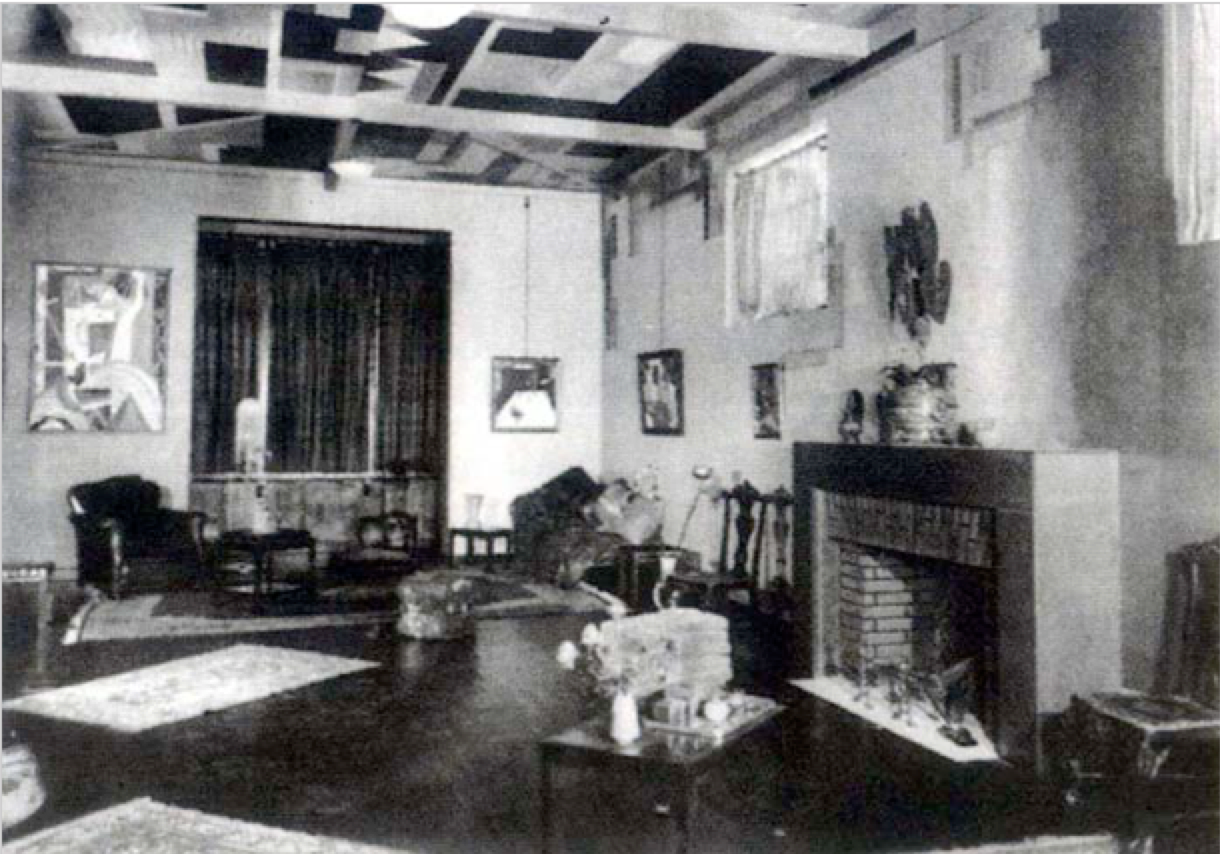
\includegraphics[width=100mm]{./imgs/fig3.jpg}
%\caption{Figura 3. Pavilhão Moderno. D. Olivia Guedes Penteado. 1925.}
%%\end{minipage}
%\end{figure}


\textls[-5]{Mário de Andrade coloca entre as suas ``maiores venturas admirar essa
mulher excepcional que foi Dona Olívia Guedes Penteado. A sua discreção,
o tato e a autoridade prodigiosos com que ela soube dirigir, manter,
corrigir essa multidão heterogênea que se chegava a ela, atraída pelo
seu prestígio, artistas, políticos, ricaços, cabotinos, foi
incomparável.''\footnote{Ibidem, p. 239, 240.} Gilda de Mello e Souza,
que estabeleceu a comparação entre esses dois espaços\footnote{Mello e
  Souza, Gilda de. \emph{A ideia e o figurado}, p. 104--106.}, não
deixa, entretanto, de pontuar o ritmo contraditório dessas
transformações ``modernizantes'' que aconteciam em São Paulo e o
esgarçamento resultante daquela tentativa de costura entre ``retalhos''
tão diversos:}

\begin{quote}
Um detalhe, no entanto, demonstra que a conquista da modernidade ainda
era recente e delicada, e que apesar de sua liberalidade a dona da casa
continuava impondo aos novos amigos o código severo de seu mundo: o
pavilhão fora construído no jardim, mantendo"-se, por conseguinte,
cautelosamente segregado do corpo da residência, e como recebia em dias
precisos --- sempre nas terças"-feiras --- excluía"-os de um contato
eventual com seus frequentadores costumeiros. Aliás, o tom das reuniões
não era ditado, propriamente, pela presença dos modernistas, mas pela
personalidade de D. Olívia, cuja autoridade todos acatavam com respeito.
O salão acabava sendo, assim, mais importante para ela que para os
convidados, pois lhe permitia, sem grande risco, brincar de vanguarda em
seus jardins, como Maria Antonieta brincara de pastora no Petit
Trianon.\footnote{Ibidem, p. 106--107.}
\end{quote}

\section*{Mário de Andrade, modernismo e política}

Nessa toada, a década de 1920 era marcada também pela atuação intensa
desse jovem alto, corpulento e de sorriso largo que se tornou uma figura
central do movimento modernista: Mário de Andrade. O escritor procurava
participar da vida da cidade, frequentando os diversos espaços em que
aconteciam os salões da época, eventos artísticos, concertos musicais,
óperas e toda sorte de eventos culturais que a cidade, em acelerada
expansão, oferecia. Parte de São Paulo --- a esse tempo ainda muito menor
e mais provinciana do que a atual metrópole gigantesca --- assistia,
entre descrente e risonha, às ações desse modernista paulistano que
andava interessado em forçar dimensões criativas e caminhos impensados
na realidade cotidiana. Na famigerada Semana de 1922, Mário de Andrade
leu alguns versos de \emph{Pauliceia desvairada,} livro de poemas que
seria lançado meses depois e que possui uma mistura irreverente de
correntes artísticas modernas --- surrealismo, futurismo, dadaísmo --- e
soluções teóricas inusitadas no famoso ``Prefácio interessantíssimo''.
Posição que o autor modula em suas obras seguintes, do estilo coloquial
dos poemas de \emph{Losango cáqui} à carga etnográfica de \emph{Clã do
Jabuti}, livros que prenunciam o choque de \emph{Macunaíma}, em 1928,
obra central da literatura brasileira, que costura, em uma prosa
literária original, o principal da reflexão estética do autor. Ainda
nesse mesmo ano de 1928, aconteceria, dentro da sua vocação de
polígrafo, a publicação do \emph{Ensaio sobre a música brasileira}, hoje
um clássico da musicologia nacional e orientador de tantas realizações
musicais posteriores.

O espírito modernista dos anos 20, que causava espanto e risadas (o
próprio Mário conta que não conseguia parar de gargalhar na exposição da
pintora Anita Malfatti em 1917), já na virada para os anos 30 ``se
alastra pelo país e transforma em estado de espírito coletivo o que era
pensamento de poucos; em realidade atuante o que era plano ideal; em
gosto habitual o que parecia aberração de alguns''. Nesse momento, Mário
começa a considerar mais seriamente que o trabalho do movimento
modernista --- ainda fragmentado em direções estéticas e políticas
divergentes na década de 1920 --- poderia se desdobrar também em novas
possibilidades nos planos político e social.

É possível acompanhar essa inflexão política no seu discurso em uma
crônica publicada no jornal \emph{Diário Nacional} em 17 de novembro de
1929, na qual afirma que a fundação (em 1926) do Partido Democrático
decorria do ``movimento de renovação brasileira, aberto faz mais ou
menos dez anos.''\footnote{Andrade, Mário de. \emph{Táxi e crônicas do
  Diário Nacional}, p. 159.} A medida dessa década de ``renovação''
parece incluir eventos como, entre outros, o fim da 1ª guerra mundial, a
exposição de Anita Malfatti de 1917, a Semana de Arte Moderna, a
Exposição Internacional do Centenário da Independência, a greve geral de
1917, a Revolução Russa, a fundação do Partido Comunista e, de maneira
muito mais imediata para a fundação do Partido Democrático, a Revolução
de julho de 1924 que ``confirmou {[}\ldots{}{]} o atraso político das
elites''\footnote{\textls[-25]{Martins, José de Souza. \emph{São Paulo no século \versal{XX}}, p. 81. ``Em São Paulo, o Partido Republicano Paulista estava dividido
  havia muito tempo. Os dissidentes já haviam sido colocados sob
  suspeita de conspiração com os revoltosos da Revolução de 1924, coisa
  que nunca ficou clara. Da dissidência, acabaria surgindo o Partido
  Democrático, que apoiou a Revolução de 1930''.}}.

O Partido Democrático havia surgido para fazer oposição ao acordo
oligárquico conhecido como ``República do café"-com"-leite'' e, portanto,
ao \versal{PRP} (Partido Republicano Paulista). Apoiou, então, alguns anos
depois, a chapa encabeçada por Getúlio Vargas contra o candidato
paulista da situação, Júlio Prestes. Como se sabe, o partido da situação
venceu o pleito, mas não durou, acusado de fraude eleitoral. A tomada do
poder por Vargas em 1930 marcou, nesse processo, o início da assim
chamada ``Nova República''. Os acordos estabelecidos de então se
desestruturavam, e o novo governo passou a imprimir novos ritmos aos
discursos de efetivação dos valores democráticos e seguridade social,
refletidos, entre outras coisas, na criação dos novos Ministérios do
Trabalho, Indústria e Comércio e o Ministério da Educação e Saúde. No
âmbito da reforma que estava sendo promovida por essas novas políticas,
Mário de Andrade e Luciano Gallet chegam a preparar já em 1931 um
Projeto de Reforma da Organização Didática do Instituto Nacional de
Música.\footnote{\emph{Reforma do Instituto Nacional de Música (1931)}.
  Série Manuscritos, caixa 122, Arquivo Mário de Andrade, \versal{IEB/USP}.}

Mas em pouco tempo surgiriam divergências entre os paulistas e o governo
provisório. A nomeação do tenente pernambucano João Alberto Lins de
Barros como interventor em São Paulo causou a fúria dos democráticos,
que tinham esperanças de assumir o governo estadual. O chefe de polícia
e democrático Vicente Rao, por exemplo, seria tirado apenas quarenta
dias depois de assumir, acusado pelo governo de atuação ``pautada por
certo espírito de partidarismo que o tornava incompatível com o cargo''.
Junto com ele sairiam outros membros do partido como Paulo Duarte e
Carlos Morais de Andrade, o primeiro, amigo próximo, e o segundo, irmão
de Mário de Andrade. As animosidades cresciam, e a oposição dos
democráticos ao governo provisório levou à criação da Frente Única
Paulista, que agora unia os então adversários (democráticos e
republicanos) em favor da autonomia de São Paulo, visando tomar o
governo provisório de Vargas. Em 23 de maio de 1932 (data que virou nome
de avenida), o país assistia a uma grande manifestação organizada pelo
movimento paulista, cujo confronto com os tenentistas resultou em mortos
e feridos. Pouco tempo depois, em 9 de julho de 1932 (outro nome de
avenida), tem início a chamada Revolução Constitucionalista, na qual os
paulistas tentam assumir o controle do governo. Uma guerra civil
violenta se desenvolve por meses, terminando com a derrota de São Paulo.

\textls[-15]{O armistício assinado entre revoltosos paulistas e o governo Vargas
inclui a nomeação para interventor em São Paulo, em
agosto de 1933, do ``civil e paulista'' Armando de Salles Oliveira,
importante empresário, além de cunhado de Júlio de Mesquita Filho,
diretor do jornal \emph{O Estado de São Paulo}. Promulgada a
Constituição de 1934 e negociada uma anistia aos revoltosos de 1932,
Salles Oliveira elege"-se, agora por meio da Assembleia constituinte,
governador em abril de 1935.}

\textls[-5]{Membros ligados ao Partido Democrático vão compondo o governo de Salles
Oliveira, entre eles alguns ligados ao movimento modernista. Ainda em
1934, o então interventor nomeava como prefeito da cidade de São Paulo o
vereador Fábio da Silva Prado, sobrinho do conselheiro Antônio Prado,
primeiro prefeito da cidade, que governara por 12 anos. Fábio Prado era
casado com Renata Crespi, filha de Rodolfo Crespi, um dos mais
importantes empresários do país ao lado de, e concorrendo com, Francesco
Matarazzo\footnote{Ambos imigrantes que fizeram carreira no Brasil e
  ganharam do governo italiano o título de conde.}. O prefeito
recém"-nomeado, Fábio Prado, escolheu como seu chefe de gabinete Paulo
Duarte, antigo redator"-chefe do \emph{Estado de São Paulo} que havia
participado com Júlio de Mesquita Filho da criação e organização da
Universidade de São Paulo.}

Paulo Duarte tinha larga trajetória de atuação política, tendo
participado da campanha de Rui Barbosa para presidente em 1919, da
revolta tenentista de 1924, da fundação do Partido Democrático em 1926,
da redação do \emph{Diário Nacional} e, também, da caravana de Vargas e
de sua ida a São Paulo em 1930. Como muitos democráticos, passa a fazer
oposição ao governo, e em 1931 participa da fundação da Liga de Defesa
Paulista, defendendo o rompimento do Partido Democrático com o governo
provisório e ajudando a organizar o levante paulista de 1932. Com a
derrota é exilado, mas volta na interventoria de Salles Oliveira,
tornando"-se, então, chefe de gabinete do prefeito Fábio Prado em 1934 e
deputado na Assembléia Constituinte estadual em 1935. É ele quem propõe
ao prefeito a criação de um Departamento de Cultura na cidade de São
Paulo --- projeto que havia sido sonhado em uma roda de amigos entre o
final dos anos 1920 e o começo dos 1930\footnote{Essa roda de amigos
  acontecia em um apartamento na Av. São João que Paulo Duarte dividia
  com Nino Gallo e contava com, além de outros eventuais, Mário de
  Andrade, Antônio de Alcântara Machado, Tácito de Almeida, Sérgio
  Milliet, Antônio Carlos Couto de Barros, Henrique da Rocha Lima,
  Rubens Barbosa de Moraes e Randolfo Homem de Melo, muitos deles
  aproveitados em diferentes funções no Departamento.}.

\section*{O Departamento de Cultura}

Elide Rugai Bastos já comentou que a criação de um Departamento de
Cultura em São Paulo marca a ``liberação de um modelo de mecenato
característico da política oligárquica. O próprio rompimento político
leva à transformação: o Estado será o novo mecenas''\footnote{Barbato
  Júnior, Roberto. \emph{Missionários de uma utopia nacional"-popular: os
  intelectuais e o Departamento de Cultura de São Paulo}, p. 13.}. Paulo
Duarte também descreve essa passagem em seu livro de memórias:

\begin{quote}
\textls[-20]{Mas cadê dinheiro? O nosso capital eram sonhos, mocidade e coragem.
Havia quem conhecesse uns homens ricos de São Paulo, mas o homem rico
não dá dinheiro pra essas loucuras. Quando muito deixa para a Santa
Casa. Caridade espiritual, jamais. Que testamento pinchou legado para
uma universidade ou para uma biblioteca? A nossa gente ainda está no
paleolítico da caridade física. À vista de tantos argumentos, ficou
decidido que um dia seríamos governo. Só para fazer tudo aquilo com
dinheiro do governo.\footnote{Duarte, Paulo. \emph{Mário de Andrade por
  ele mesmo}, p. 50.}}
\end{quote}

O projeto do Departamento foi apresentado ao prefeito por Paulo Duarte
tendo como exigência que o cargo de diretor fosse ocupado por aquele
mesmo modernista e amigo próximo do solicitante, Mário de Andrade.
Exigência que foi atendida em acordo com o governador Salles Oliveira,
este também vinculado ao Partido Democrático e amigo íntimo de Paulo
Duarte, ``velha amizade'' que se estabeleceu ``na luta e no
exílio''\footnote{Cf. Raffaini, Patricia Tavares. \emph{Esculpindo a
  cultura na forma Brasil: o Departamento de Cultura de São Paulo
  (1935--1938)}, p. 38.}. O projeto desse grupo de amigos é interpretado
por alguns analistas como

\begin{quote}
parte de uma ideia hegemônica, por meio do qual o estado de São Paulo,
depois da derrota da Revolução de 1932, conseguiria, na visão dos que
planejavam o Departamento de Cultura e as recém"-criadas faculdades,
conquistar e transformar o resto do país através da cultura e da
educação.\footnote{Ibidem, p. 35.}
\end{quote}

Alguns historiadores e sociólogos pensam ter havido uma aposta
reformista no âmbito educacional e cultural, como parte das políticas
paulistas desde a prefeitura de Antônio da Silva Prado, que inclui a
construção do Teatro Municipal (concluída em 1911), a organização do
sistema educacional público feita na prefeitura de Washington Luís e a
organização dos parques infantis realizada na gestão Anhaia Mello, que
seguiam as bases de um projeto que Fernando Azevedo apresentou para a
prefeitura em 1923. No governo de Armando de Salles Oliveira fora
construído um prédio para a Biblioteca Pública Municipal, unidades
escolares de ensino primário e secundário, a Faculdade de Filosofia, que
começava a formar professores para o ensino público, e a própria
Universidade de São Paulo. Nessa linha de interpretação, parece ter
havido um esforço paulista de fazer com que o \emph{boom} econômico da
passagem do século fosse acompanhado da criação de instituições
culturais que dessem uma identidade paulista ao processo, gerando uma
alternativa à hegemonia cultural da capital federal. Na opinião de
Carlos Sandroni, ``a questão cultural esteve intimamente ligada à
possibilidade de resgatar o papel hegemônico de São Paulo dentro da
federação''.\footnote{Sandroni, Carlos. \emph{Mário contra macunaíma:
  cultura e política em Mário de Andrade}, p. 75.}

Realizações da década de 30 como o Departamento de Cultura, a Escola
Livre de Sociologia e Política e a Universidade de São Paulo teriam
ganho impulso no contexto da reação paulista às sucessivas derrotas
políticas. Isso se daria em boa medida por meio de uma recomposição da
elite intelectual (e econômica) e da reabilitação do sentimento de amor
próprio que tem como horizonte colocar São Paulo novamente em uma
posição de destaque no país, como --- para usar o jargão da época --- a
locomotiva da nação. A ideia descrita por Paulo Duarte era conduzir
Armando de Salles Oliveira à presidência em 1938, tendo como carro"-chefe
uma plataforma forte de bem"-estar social promovida por meio de
instituições culturais que de fato funcionassem. O Departamento de
Cultura foi pensado como etapa inicial e experimental desse projeto
maior, que posteriormente seria aplicado como política nacional na forma
de um ``Instituto Brasileiro de Cultura'':

\begin{quote}
Nós sabíamos que o Departamento {[}de Cultura{]} era o germe do
Instituto Brasileiro de Cultura. Primeiro, um Instituto Paulista, que
Armando Sales no governo já nos garantira. Para isso o projeto do
Departamento do Patrimônio Histórico e Artístico de São Paulo lá estava
na Assembléia Legislativa (\ldots{}) Depois, com Armando Sales na Presidência
da República, seria o Instituto Brasileiro, uma grande fundação
libertada da influência política, com sede no Rio, inicialmente
instalados, além do de S. Paulo, paradigma, outros núcleos em Minas, no
Rio Grande do Sul, na Bahia, em Pernambuco e no Ceará. Tiveramos uma
grande ideia que Armando Sales aprovou: os Institutos de Cultura
assistiriam com assiduidade todas as grandes cidades, com a colaboração
da Universidade, porque, não comportando evidentemente essas cidades uma
faculdade, teriam contato íntimo com esta, através de conferências,
cursos, teatro, concertos etc.''\footnote{Duarte, Paulo. \emph{Mário de
  Andrade por ele mesmo,} p. 55.}
\end{quote}

Instalado o Departamento de Cultura, esse sentimento de reconstrução do
orgulho paulista é, de fato, perceptível na fala do então prefeito Fábio
Prado:

\begin{quote}
O Departamento de Cultura não podia deixar de ser bem recebido no São
Paulo novo, no São Paulo pós"-revolução, onde as iniciativas culturais se
desenvolvem com o vigor das lavras na terra roxa. A universidade,
recém"-criada, aí estava florescente dando"-nos um ambiente ensolarado de
cultura. (\ldots{}) transfundindo para as veias bandeirantes o sangue
novo da cultura europeia (\ldots{}) a \versal{USP} precisava ter institutos
colaboradores de sua obra formidável.\footnote{Entrevista do prefeito
  Fábio Prado ao jornal O Estado de São Paulo, 1/03/1936. Republicada em
  Calil, Carlos Augusto e Penteado, Flávio Rodrigo. \emph{Me esqueci
  completamente de mim, sou um departamento de cultura}, p. 66.}
\end{quote}

O discurso de seu primeiro diretor, Mário de Andrade, também parece
estar afinado nesse tom:

\begin{quote}
Tudo é novo, e muito está apenas nascendo. São Paulo é uma cidade dum
dia, mas já os seus caminhos vão e vêm. O Departamento de Cultura que
tudo isto já está fazendo, com toda sua autonomia municipal, cresce e
quer crescer como a flor, como o perfume irradiante doutra criação mais
básica, a Universidade de São Paulo. E, sendo municipal, o Departamento
de Cultura cresce e quer crescer, esculpido na forma do
Brasil.\footnote{Revista da Arquivo Municipal, v.19 p. 272, 1936.
  Transcrito no cuidadoso estudo de Patricia Tavares Raffaini que tem o
  título elaborado a partir desse trecho: ``Esculpindo a cultura na
  forma Brasil''.}
\end{quote}

Para Antonio Candido, tratou"-se de um momento inédito e radical: ``não
apenas a rotinização da cultura, mas a tentativa consciente de
arrancá"-la dos grupos privilegiados para transformá"-la em fator de
humanização da maioria, através de instituições planejadas''. Candido
continua:

\begin{quote}
Nas sociedades de extrema desigualdade, o esforço dos governos
esclarecidos e dos homens de boa vontade tenta remediar na medida do
possível a falta de oportunidades culturais. Nesse rumo, a obra mais
impressionante que conheço no Brasil foi a de Mário de Andrade no breve
período em que chefiou o Departamento de Cultura da cidade de São Paulo,
de 1935 a 1938. Pela primeira vez entre nós viu"-se uma organização da
cultura com vista ao público mais amplo possível.\footnote{Candido,
  Antonio. ``O direito à literatura'', \emph{Vários escritos}, p. 258.}
\end{quote}

A proposta do Departamento era, ainda que repleta de
contradições\footnote{Contradições ligadas a uma visão beletrista e
  elitista de cultura e à pouca consideração efetiva de uma cultura
  urbana que se formava com a participação dos imigrantes, que se
  tornaram parcela significativa da população. Para essas questões,
  conferir o já citado estudo central sobre o Departamento de Cultura
  feito por Patricia Tavares Raffaini.}, avançada para o país, à medida
que conectava a cultura às suas interfaces de lazer, esporte,
assistência social, turismo, meio ambiente, planejamento, entre tantas
outras vocações, contando para sua viabilização com fabulosos 10\% do
orçamento da prefeitura. Fundado por um ato municipal a 30 de maio de
1935, o Departamento de Cultura contou com as divisões de Expansão
Cultural (chefiada por Mário de Andrade), Bibliotecas (Rubens Borba de
Moraes), Educação e Recreios (Nicanor Miranda), Documentação Histórica e
Social (Sérgio Milliet). Viria projetar e conduzir coisas como, entre
muitas, parques infantis que contavam com educadores sanitários,
pediatras, nutricionistas, instrutores de jogos e professores; programas
de distribuição de leite para crianças; bibliotecas infantis,
circulantes e populares de bairro; um restaurante público dedicado a
receitas brasileiras; concursos de composição musical, roteiros de
teatro e decoração proletária (!); estudos da conformação urbana de São
Paulo; pesquisas sociais e etnográficas para detectar problemas de
alimentação, moradia e educação; mapas folclóricos para localização de
danças e culturas típicas, entre tantas outras iniciativas
pioneiras\footnote{Para uma descrição mais detalhada de todas essas
  atividades ver, entre outros, as publicações de Carlos Augusto Calil e
  Flávio Penteado (2015), Roberto Barbato Jr. (2004), Patricia Raffaini
  (2001), Carlos Sandroni (1988) e Flávia Toni (1984).}.

Depois das experiências modernistas mais radicais da década de 20,
estava se consolidando, nos anos 30, uma dimensão mais construtiva,
engajada na tentativa de integrar o esgarçado tecido social paulista e
nacional, numa visada que buscou ao mesmo tempo formar um conjunto
estável, e em boa medida problemático, das ``coisas brasileiras''. Ou
ainda, na formulação de Mário: ``é justo por esta data de 1930, que
principia para a Inteligência brasileira uma fase mais calma, mais
modesta e quotidiana, mais proletária, por assim dizer, de construção. À
espera que um dia as outras formas sociais a imitem''\footnote{Andrade,
  Mário de. ``O movimento modernista'', \emph{Aspectos da Literatura
  brasileira}, p. 242.}. Em entrevista ao jornal, já como diretor do
Departamento de Cultura, o escritor perguntava: ``não será esse o mal
maior do Brasil? Essa ausência de um ``homem brasileiro'', de um ser uno
e coletivo que persista dentro de todos nós e seja nossa unidade
nacional? O Departamento não pode ficar indiferente a esse problema
capital.''\footnote{\emph{O Estado de S. Paulo}, 21 de fevereiro de
  1936, p. 3. Republicado em Calil e Penteado, \emph{Me esqueci
  completamente de mim, sou um departamento de cultura}, p. 65.} Como
solução, propunha ``colher, colher cientificamente nossos costumes,
nossas tradições populares, nossos caracteres raciais, esta deve ser a
palavra de ordem dos nossos estudos etnográficos (\ldots{}) enquanto o
progresso e o internacionalismo não destroem os nossos costumes e as
bases culturais da nossa gente''\footnote{``Minuta da palestra de
  inauguração do Curso de Etnografia''. {[}Mário de Andrade, 1936{]}.
  Transcrito em Cardim, Vera Lúcia. \emph{Contribuições de Samuel Lowrie
  e Dina Lévi"-Strauss ao Departamento de Cultura de São Paulo (1935--1938).}}.

O processo de escolha e seleção que levaria à construção desse ``ser uno
e coletivo'', ou essa tentativa de chegar a um ``homem brasileiro'' como
um padrão de base para a organização das políticas culturais, não deixa
de ser uma empreitada que aos ouvidos atuais, ao menos alguns, soa como
algo um tanto restritivo, ou pouco plural, ainda mais se considerarmos a
rica cultura urbana que se formava na cidade de São Paulo no atrito com
os imigrantes. Isso, no entanto, permitiu que muitas manifestações
culturais, principalmente de zonas rurais brasileiras, fossem
registradas e documentadas.

É nesse contexto que a Divisão de Expansão Cultural projeta uma
Discoteca Pública e uma Rádio"-Escola. A ideia desses projetos sonoros
ganha importância se lembrarmos que nesse início de século grande parte
dos cidadãos brasileiros --- e paulistas --- não sabiam ler ou tinham
leitura precária. Podemos acompanhar a luta pela instalação da
Rádio"-Escola e sua orientação em um ofício da Diretoria do Departamento,
solicitando

\begin{quote}
A colocação definitiva, e não provisória, duma rede de alto"-falantes,
nos logradouros públicos da cidade. É justamente aos jardins que acodem
as populações proletárias e de pequena burguesia, que dispõem de poucos
meios para se divertir. É justamente a essas classes que a ação cultural
da Rádio Escola terá de se dirigir com preferência, não só por serem as
demais, passível de educação e sugestão, como por serem as menos
providas de meios para se cultivar. Por todas estas razões, julga esta
Diretoria, não só da maior utilidade, mas imprescindível à organização
dum sistema irradiador público, que obrigue o povo a escutar a Rádio
Escola, e permita ouvi"-la aos que não têm rádios em casa\footnote{Ofício
  de 17 de fevereiro de 1936, Processo 23937, reproduzido em Calil e
  Pacheco, p. 51. O diretor do Departamento de Cultura estava imerso em
  uma série de contradições e ambiguidades que marcavam seu lugar
  social, e a possibilidade de ``levar cultura à população'' é formulada
  em chave paternalista.}.
\end{quote}

Ao que parece, ao menos nesse momento, o discurso e o léxico do grupo de
intelectuais do Departamento de Cultura se aproximava ao de uma
social"-democracia de tipo europeu, entendendo como uma das funções da
política a de diminuir os estragos da roda"-viva capitalista --- cuja
vocação é concentrar as riquezas e aumentar infinitamente a diferença
entre pobres e ricos. Nicanor Miranda, por exemplo, chefe da divisão de
Educação e Recreios, escrevia sobre como as ações de sua seção visavam a
integração dos ``adolescentes operários'':

\begin{quote}
\textls[-25]{Não serão os adolescentes operários os homens de amanhã, que bem ou mal
integrados na sociedade constituirão a massa de trabalhadores da nação?
Porque não integrá"-los bem, proporcionando"-lhes quanto antes, os meios e
os recursos para que venham a ser profissionais aptos, cidadãos nobres e
dignos das suas funções na coletividade?\footnote{\textls[-60]{\emph{Clube de menores
  operários}, separata da rev. Arq. Mun. 1938 vol. \versal{XLVIII}, p. 81.}}}
\end{quote}

Roberto Barbato Júnior diz que nesse momento o grupo de intelectuais
buscou ``organizar um amplo espectro de difusão cultural que minimizasse
o aspecto de excludência imposto à população''\footnote{Barbato Júnior,
  Roberto. \emph{Missionários de uma utopia nacional"-popular: os
  intelectuais e o Departamento de Cultura de São Paulo,} p. 16.}.
Adeptos de algo como uma ``esquerda moderada''\footnote{A expressão é de
  Antonio Candido. ``Prefácio'', em Duarte, Paulo. \emph{Mário de
  Andrade por ele mesmo}.}, acreditaram que a política poderia cumprir a
função de consertar os abismos sociais produzidos pela circulação do
capital \emph{sem precisar depor seus agentes acumuladores}, ou seja,
sem depor a elite --- sem desejar uma revolução. Em uma carta a Paulo
Duarte, Mário de Andrade explica:

\begin{quote}
Num país como o nosso, em que a cultura infelizmente não é ainda uma
necessidade quotidiana de ser, está se aguçando com violência dolorosa o
contraste entre uma pequena elite que realmente se cultiva e um povo
abichornado em seu rude corpo. Há que forçar um maior entendimento
mútuo, um maior nivelamento geral de cultura, que, sem destruir a elite,
a torne mais acessível a todos, e em consequência lhe dê uma validade
verdadeiramente funcional. Está claro, pois, que o nivelamento não
poderá consistir em cortar o tope ensolarado das elites, mas em provocar
com atividade o erguimento das partes que estão na sombra, pondo"-as em
condição de receber mais luz. Tarefa que compete aos governos.\footnote{Duarte,
  Paulo. \emph{Mário de Andrade por ele mesmo}, p. 152.}
\end{quote}

\section*{A dor que vive aqui}

O desenrolar da década de 30 viria mostrar que a aposta naquele tipo de
``esquerda moderada'' não conseguiria operar nem o sonhado erguimento
das partes que estavam na sombra e nem reduzir o contraste entre a elite
e povo ``abichornado''\footnote{O próprio Mário modulará sua posição
  política, e na ópera inacabada ``Café'' o povo praticamente faz uma
  revolução comunista no palco.}. O golpe de Vargas e a instalação de
uma ditadura em 1937 redundou na demissão de Mário de Andrade do
Departamento de Cultura, e viria deixar mais ou menos claro que, como já
dizia o mestre Machado de Assis --- em alemão! ---, o Brasil continuava em
boa medida estando mais para eine absolute Oligarchie\footnote{Machado
  de Assis, crônica de 11 de maio de 1888: ``Es dürfte leicht zu
  erweisen sein, dass Brasilien weniger eine konstitutionelle Monarchie
  als eine absolute Oligarchie ist'' {[}Seria fácil provar que o Brasil
  é menos uma monarquia constitucional do que uma oligarquia
  absoluta{]}.}, e os valores democráticos e culturais se realizariam
apenas na medida em que fossem necessários para manter uma certa
oligarquia no poder e uma parcela crescente do povo ``abichornando"-se''.
Em 1939, Mário escrevia o conto ``Briga das pastoras'', no qual o
narrador (com um quê auto"-referente) conta sua aventura ``etnográfica''
para assistir a um Pastoril:

\begin{quote}
Chegamos, e logo aquela gente pobre se arredou, dando lugar para os dois
ricos. Num relance me arrependi de ter vindo. Era a coisa mais
miserável, mais degradantemente desagradável que jamais vira em minha
vida. Uma salinha pequeníssima, com as paredes arrimadas em mulheres e
crianças que eram fantasmas de miséria, de onde fugia um calor de forno,
com um cheiro repulsivo de sujeira e desgraça. Dessa desgraça horrível,
humanamente desmoralizadora, de seres que nem sequer se imaginam
desgraçados mais.\footnote{Andrade, Mário de. ``Briga das Pastoras'', em
  \emph{Obra Imatura}, p. 181, 182. Conto referido em palestra de Ivan
  Marques no Instituto \versal{CPFL} Cultura no dia 23/11/2018.}
\end{quote}

O escritor descreve literariamente sua tristeza ao constatar que os performadores da cultura
popular brasileira não haviam saído da sombra, seguiam abichornados, em
ambiente repulsivo, miseráveis a ponto de brigar entre si por esmolas e
roubar dinheiro colocado no presépio. Para Mário, um povo tão afastado
das garantias sociais mínimas que vive em pânico, mendigando apoio
paternal de qualquer ``rico'', imolando"-se uns aos outros por esmola e
se arrastando numa triste miséria financeira e moral.

Talvez a impressionante empreitada construtiva do Departamento de
Cultura na gestão de Mário como seu diretor, entre 1935 e 1938, carregue
algo de reativo --- ou mesmo descompensado --- em relação a esse deserto
de instituições culturais e de garantias sociais mínimas do Brasil. Algo
de galicismo a berrar nos desertos da América. Talvez por isso, depois
de passar por essa experiência, Mário tenha se lembrado de incluir no
diário da viagem de 1927 (que fizera junto a Dona Olívia Guedes
Penteado) uma carta endereçada a uma ``amiga judia comunista francesa'',
Dina Dreyfus, que havia retornado à França depois de ter dado tantas
contribuições ao Departamento de Cultura. Na carta, Mário escreve:

\begin{quote}
N'avez vous pas senti nos peurs américaines, et nos impossibles? {[}Não
captou os nossos medos americanos e nossas impossibilidades?{]} O que é
Hitler, Daladier, a impotência, a clarividência criminosa? Os vossos
operários europeus? Eles não sofrem não, eles teorizam sobre o
sofrimento. A dor, a imensa e sagrada dor do irreconciliável humano,
sempre imaginei que ela viajara na primeira caravela de Colombo e vive
aqui. Essa dor que não é de ser operário, que não é de ser intelectual,
que independe de classes e de políticas, de aventureiros Hitlers e de
covardes Chamberlains, a dor dos irreconciliáveis vive aqui.\footnote{Andrade,
  Mário de. \emph{O Turista aprendiz,} p.174.}
\end{quote}

Para Mário, a dor do irreconciliável é específica, uma dor
``sul"-americana do indivíduo (\ldots{}) de incapacidade realizadora do ser
moral'', diferente do lamento comunista, europeu, derivado do circuito
estrito e racional do iluminismo. No Brasil, ``nós é esta irresolução,
esta incapacidade (\ldots{}) uma dor permanente, a infelicidade do acaso pela
frente''. Aportadas com as caravelas de Colombo e colocadas para
funcionar em chão diverso, as ideologias modernas europeias na América
deslizavam (deslizam?), e nesse deslizar, como todo deslizamento,
performam uma parcela de descontrole e irracionalidade. O espaço
deslizante faz com que o conjunto de normas modernas se sustente com
dificuldade, pisando em ovos, fazendo patinar as categorias tradicionais
de autonomia, liberdade, direito ou justiça\footnote{Cf. Schwarz,
  Roberto. ``As ideias fora do lugar'', em \emph{Ao vencedor as
  batatas}.}. Para Mário de Andrade, essa dor, sul"-americana,
específica, brasileira, era outra em relação à dor europeia que sua
amiga francesa sentia em sua luta por direitos, operária,
revolucionária. A amiga comunista tinha atrás de si a experiência da
Revolução Francesa, da Primavera dos Povos, da Comuna de Paris, da
Revolução Russa. No Brasil de Mário, cheio de galicismos decorativos, os
momentos de acumulação de conflitos de classe que poderiam ter levado à
criação de mais igualdade e seguridade social eram cortados por golpes e
massacres daquela absolute oligarchie. Golpe da maioridade, golpe da
República, massacre de Canudos, golpe do Estado Novo, 1964, Carandirú,
Carajás\ldots{} uma história que ainda preside nossos dias, e assombra.
Os golpes se repetiam, e após o golpe de Vargas, Mário de Andrade,
demitido, escrevia ao amigo que o indicara para o cargo de diretor:

\begin{quote}
Sacrifiquei por completo três anos de minha vida começada tarde,
dirigindo o Departamento de Cultura. Digo \emph{por completo} porque não
consegui fazer a única coisa que, em minha consciência, justificaria o
sacrifício: não consegui impor e normalizar o D. C. na vida paulistana.
{[}\ldots{}{]} Não me sinto propriamente triste com estas coisas, me sinto
especialmente deserto. É uma vagueza, uma vacuidade monótona.\footnote{Duarte,
  Paulo. \emph{Mário de Andrade} \emph{por ele mesmo}, p. 158--159.}
\end{quote}

\begin{bibliohedra}
\tit{anderson}, Benedict. \emph{Comunidades imaginadas: reflexões sobre a origem e a
difusão do nacionalismo}. Companhia das Letras, 2008.

\tit{andrade}, Mário de. ``O movimento modernista'', \emph{Aspectos da
literatura brasileira}. Martins, 1974.

\titidem. \emph{Táxi e crônicas do Diário Nacional.} Duas
Cidades, 1976.

\titidem. ``Briga das Pastoras'', em \emph{Obra Imatura},
Martins, 1980.

\tit{barbato júnior}, Roberto. \emph{Missionários de uma utopia
nacional"-popular: os intelectuais e o Departamento de Cultura de São
Paulo}. Annablume, 2004.

\tit{calil}, Carlos Augusto e \textsc{penteado}, Flávio Rodrigo. \emph{Me esqueci
completamente de mim, sou um departamento de cultura.} Imprensa Oficial
do Estado de São Paulo, 2015.

\tit{candido}, Antonio. ``Prefácio'', em Duarte, Paulo. \emph{Mário de Andrade
por ele mesmo}. 2a ed. Hucitec, Secretaria Municipal de Cultura de São
Paulo, 1985.

\titidem. ``O direito à literatura'', \emph{Vários escritos}. 3ª
ed.. revista e ampliada. Duas Cidades, 1995.

\tit{cardim}, Vera Lúcia. \emph{Contribuições de Samuel Lowrie e Dina
Lévi"-Strauss ao Departamento de Cultura de São Paulo (1935--1938)},
dissertação de Mestrado, \versal{PUC-SP}, 2010.

\tit{graham}, Douglas e \textsc{hollanda}, Sérgio Buarque de. \emph{Migrações internas
no Brasil 1872--1970}, Instituto de Pesquisas Econômicas {[}Brasília{]}
Conselho Nacional de Desenvolvimento Científico e Tecnológico, 1984.

\tit{martins}, José de Souza. \emph{São Paulo no século \versal{XX}}. Imprensa oficial
do Estado de São Paulo, 2011.

\tit{mello} e Souza, Gilda de. \emph{A ideia e o figurado}. Duas
Cidades/Editora 34, 2005.

\tit{miceli}, Sérgio. \emph{Nacional estrangeiro}. Companhia das Letras, 2003.

\tit{pontes}, Heloísa. \emph{Destinos Mistos}. Companhia das Letras, 1998.

\tit{raffaini}, Patricia Tavares. \emph{Esculpindo a cultura na forma Brasil:
o Departamento de Cultura de São Paulo (1935--1938)}. Humanitas
\versal{FFLCH/USP}, 2001.

\tit{sandroni}, Carlos. \emph{Mário contra macunaíma: cultura e política em
Mário de Andrade}. Vértice/Iuperj, 1988.

\tit{schwarz}, Roberto. \emph{Ao vencedor as batatas: forma literária e
processo social nos inícios do romance brasileiro}. Editora 34, 2000.

\tit{sevcenko}, Nicolau. \emph{Orfeu extático na metrópole: São Paulo,
sociedade e cultura nos frementes anos 20.} Companhia das Letras, 1992.
\end{bibliohedra}

\chapter*{São Paulo fonografado}
\addcontentsline{toc}{chapter}{São Paulo fonografado, \emph{por Biancamaria Binazzi e Enrique Menezes}}
\hedramarkboth{São Paulo fonografado}{}

\begin{flushright}
\textsc{biancamaria binazzi\\ enrique menezes}
\end{flushright}

A Discoteca Pública Municipal (hoje Discoteca Oneyda Alvarenga, no
Centro Cultural São Paulo), justificava nessas palavras curiosas um
pedido de verba pública para ser usada em 1937 em seu serviço de
gravação de discos:

\begin{quote}
A discografia nacional, erudita e popular, é sumamente pobre. As casas
gravadoras seguem naturalmente seus interesses comerciais e nada fazem,
no domínio da música erudita, de artisticamente recomendável, e no
domínio da música popular --- de folcloristicamente sério. Nem se pode
esperar que esse programa de trabalho das casas gravadoras seja
melhorado enquanto o público mesmo não começar a exigir coisa melhor.
(\ldots{}) é natural que não se possa confiar às casas gravadoras o destino
exclusivo de nossa música registrada.\footnote{\emph{Justificação da
  Verba para 1937 sobre gravação de discos}. São Paulo (município).
  Secretaria Municipal de Cultura. Centro Cultural São Paulo. Acervo
  Histórico Discoteca Oneyda Alvarenga. Fundo Discoteca Pública
  Municipal, pasta 1935 a 1939, não catalogado.}
\end{quote}

Fundada em 1936, como uma iniciativa do Departamento de Cultura de São
Paulo, a Discoteca tentava criar uma outra via em relação aos interesses
comerciais da então recente e lucrativa indústria fonográfica. Foi a
primeira discoteca brasileira a inaugurar um serviço de gravação sonora
etnográfica, além de registrar e lançar, em disco, a música de concerto
de compositores paulistas. Aproximava assim as duas pontas fora da curva do novo mercado musical: a gravação de
performances de música popular captadas em seus lugares originais e a
música de concerto contemporânea.

Sob direção da poetisa e musicóloga Oneyda Alvarenga, a Discoteca
amplificava o sonho admirável e problemático dos intelectuais do
Departamento de Cultura de modelar uma identidade nacional a partir da
cultura popular. Como uma biblioteca sonora, oferecia cabines para
audição, promovia concertos de discos, congressos, concursos,
publicações e estudos sobre a cultura musical brasileira. Ali, qualquer pessoa
poderia (ainda pode) sentar numa cadeira confortável e ouvir uma coleção
de discos, consultar partituras, livros, e assistir filmes etnográficos. Em
tempos de internet, onde um sem"-fim de coisas estão acessíveis
\emph{online} a dois cliques, a importância desse tipo de iniciativa
pode parecer menor, mas façamos o esforço analógico de pensar que aquele
era um tempo no qual ainda não havia o troca"-troca furibundo das redes
virtuais.

Quando escreve \emph{Macunaíma}, por exemplo, Mário de Andrade não podia
encomendar pela Amazon, e teve que tomar complicadas providências
não"-digitais para conseguir um exemplar do livro \emph{Von Roraima zum
Orinoco}, no qual o pesquisador alemão Theodor Koch"-Grünberg relata o
mito indígena de Maku"-Naima, escutado em suas viagens pela Amazônia, na
virada para o século \versal{XX}. Nas viagens que deram origem a esse livro (que
Mário conhecia de trás pra frente) além de anotar mitos e paisagens, o
alemão usou um fonógrafo para gravar e reproduzir sonoridades
amazônicas.\footnote{Criado em 1877 por Thomas Edison, o fonógrafo era
  um aparelho mecânico, (mais ou menos) portátil que através de um cone
  metálico captava as vibrações sonoras e as marcava, com uma agulha, em
  cilindros de cera. Os cilindros de Koch"-Grünberg estão entre as
  primeiras gravações ``em campo'' feitas no Brasil, na virada do
  século, junto com as dos também alemães Richard Wettstein e Wilhelm
  Kissenberth. (O botânico austríaco Richard Wettstein esteve no Brasil
  em 1901 e 1903, e gravou, entre outras, falas e canções Guarani para o
  Arquivo Fonográfico de Viena. Por aqui, o primeiro brasileiro a gravar
  música em viagem etnográfica foi Edgard Roquete"-Pinto, que em 1912
  registrou cantos indígenas Paresí, Nambikwara, sertanejos e
  instrumentos cuiabanos, entre outras sonoridades. Note"-se nesses
  pesquisadores o interesse voltado aos sons indígenas, unânime entre os
  alemães. Ao gravar canto e instrumento de gente do Brasil central,
  Roquete"-Pinto foi pioneiro em ``gravações de campo'' da música
  tradicional brasileira não"-indígena.} Era uma possibilidade incrível:
os sons indígenas poderiam ser captados em seu lugar original na forma
de cilindros de cera e reproduzidos em qualquer lugar do mundo. Todo um
novo campo se abria.

Mário de Andrade, que se interessava tanto pela música indígena quanto
pela popular e pela de concerto, vê nessa nova tecnologia uma enorme
oportunidade, e lamentava que ainda não existissem discos ``produzidos
cientificamente'' para estudo da música tradicional brasileira. Ainda
que tenha sempre recorrido ao pentagrama para escrever música, o
escritor estava consciente da limitação de tentar traduzir os sons com
lápis e papel. Sabia que sua escrita carregava as marcas de uma certa
tradição (euro"-cristã), privilegiando as alturas em detrimento do
timbre, entonação, ``sutilezas de invenção do cantador'' e invenções
rítmicas que desafiavam as barras de compasso. A novidade da gravação
sonora poderia ultrapassar as possibilidades da escrita musical.

\begin{quote}
Nunca uma canção transcrita no papel ou no instrumento poderá dar a quem
estuda, a sua exata realidade. E a verificação dessa verdade, depois que
a fonografia veio nos apresentar o mundo de riqueza do cantar de todos
os povos da terra, tornou a grafia musical por meios não mecânicos,
bastante desautorizada como base de estudos etnográficos e
folclóricos.\footnote{Andrade, Mário. ``A pronúncia cantada e o problema
  do nasal brasileiro através dos discos'' {[}1936{]}, em \emph{Aspectos
  da Música Brasileira}, p. 96.}

(\ldots{}) Além de não registrar o timbre, os ajuntamentos de sons, e as miseráveis
polifonias e acordes resultantes desses ajuntamentos imprevistos e
talvez ocasionais, não representam sequer a realidade melódica ou
textual. Representam apenas uma constância, quero dizer: a maneira mais
frequente e predominante com que a coisa se manifestou textual e
melodicamente. (\ldots{}) Há que recorrer à gravação por meios mecânicos,
disco e filme.\footnote{Andrade, Mário. ``Samba Rural Paulista''
  {[}1937{]}, em \emph{Aspectos da Música Brasileira}, p. 118.}
\end{quote}

Sobre as imensas possibilidades que o fonógrafo trazia para a música, o
nosso escritor também se informava com outro alemão, Eric M. Hornbostel,
que considerou a crença na transcrição musical no papel uma espécie de
``superstição europeia''. Pioneiro naquilo que ficou conhecido como
``musicologia comparada'', Hornbostel começava a discutir a suposta
superioridade das concepções europeias na música. Mário traduz um trecho
de seu livro \emph{African negro music}, de 1928:

\begin{quote}
Como material para estudo, os fonogramas são imensamente superiores à
notação das melodias e não se pode conceber que este método inferior
ainda seja usado. Basta verificar que exclusivamente por meio da \label{ref1}
fonografia, é que podemos obter a coisa legítima. O pressuposto geral de
que a substância de uma canção pode ser notada em pauta com os auxílios,
talvez, de sinais diacríticos e texto explicativo, é mera superstição
europeia, ocasionada pela evolução da música e a maneira geral de pensar
dos europeus. Os próprios cantores dão tanta importância ao timbre da
voz e à dicção como a qualquer outra coisa. E mesmo às vezes mais. De
fato, dicção e timbre demonstram ser caracteres raciais profundamente
predeterminados por funções fisiológicas, e são, por isso, valiosa prova
das relações e diferenciações antropológicas. Assim, os povos e suas
músicas, não se distinguem tanto pelo que cantam como pela maneira por
que cantam.\footnote{Andrade, Mário. ``A pronúncia cantada e o problema
  do nasal brasileiro através dos discos'' {[}1936{]}, em \emph{Aspectos
  da Música Brasileira}, p. 96.}
\end{quote}

Até aquele momento, os discos de música brasileira gravada em campo em
seus contextos locais eram extremamente raros, e o escritor procurava
nos discos comerciais as performances que mais se aproximavam da
espontaneidade original. Desanimado com o que havia de música rotulada
nos discos como ``folclórica'', entre ``deformações'', ``exotismos'' e
``estilizações'', Mário pinçava raras (e preciosas) pérolas: nos
artigos ``A música no Brasil'' (de 1931) e ``A música e a canção
populares no Brasil'' (de 1936), encomendados por organizações
internacionais, o escritor explica para o público estrangeiro que para
``conhecer (e amar!)'' o brasileiro, deveriam escutar, entre outros
discos, cateretês com Mariano e Caçula, cururus com Zico Dias e
Ferrinho, modas de viola com Laureano e Soares, folia de reis com
Cornélio Pires e Maracajá, jongos com Motta da Motta, a série de
candomblé com os Filhos de Nagô, macumbas com J. B. de Carvalho, sambas
com Aracy de Almeida, choros com Pixinguinha e o ``admirável'' batuque
\emph{Babaô Miloquê} gravado por Josué de Barros. Opa! A gente, que não
é estrangeiro, agradece as dicas!

\section*{Coleções de sons pelo mundo: inspirações}

Além de ouvir música brasileira em discos comerciais nacionais, Mário
também estava informado sobre as ideias europeias que surgiam e
circulavam na virada do século \versal{XIX} para o \versal{XX}. Na ``Justificação da Verba
para 1937 sobre gravação de discos'', Mário cita criações internacionais
como a dos Arquivos Fonográficos de Berlim e Viena, o Museu da Palavra e
do Gesto na França e a seção de pesquisas musicais folclóricas por meio
do disco na Romênia:

\begin{quote}
A Alemanha tem uma notável coleção de fonogramas de nossa música
indígena, enquanto nós próprios nada possuímos a esse respeito. A
Rumania vê nascer a seção de pesquisas musicais folclóricas por meio do
disco, do Ministério das Belas Artes; vê nascer a valiosíssima,
eficientíssima Sociedade dos Compositores Rumenos. Na França, a Sorbonne
trabalha seriamente. E assim por toda a parte.

E em toda a parte, os governos quando não iniciam eles mesmos as
campanhas científicas, são patrocinadores delas. Há colaborações
internacionais, há auxílios mútuos entre organizações de países
longínquos, para preservação do que uma terra tem de mais estimável: sua
tradição, as manifestações culturais de seu povo.\footnote{\emph{Justificação
  da Verba para 1937 sobre gravação de discos.}}
\end{quote}

Nessas instituições, pesquisadores (como Hornbostel) começavam a
iluminar e discutir focos etnocêntricos de interpretações anteriores e a
espécie de eurocentrismo alucinado que com frequência menosprezava a
música de povos não europeus.\footnote{O famoso teórico Hugo Riemann
  escrevia em 1904: ``A oitava subdividida em 12 semitons (\ldots{}) é um
  fato histórico, que não se derruba com alguns apitos mal"-feitos da
  Polinésia ou com desempenhos de canto questionáveis de mulheres de
  cor''. Citado por Tiago de Oliveira Pinto em ``100 anos de
  etnomusicologia''.} Nesse impulso, antropólogos, linguistas, etnólogos
e musicólogos começavam a buscar alternativas à interpretação linear e
simplista da evolução cultural. Da convergência entre a musicologia, a
antropologia, a biologia, a psicologia e a linguística, entre outras,
começava a aparecer um campo colaborativo que,
conforme a ênfase, recebeu os nomes de musicologia comparada,
etnomusicologia e antropologia da música. Ao trabalhar nessa trilha,
Mário de Andrade procura canalizar recursos públicos para acertar os
ponteiros brasileiros com as tendências internacionais mais avançadas.

\emph{Áustria e Alemanha:} Em 1899 surgia o Arquivo Fonográfico de
Viena, ligado à Academia Imperial de Ciências. Fundada pelo psicólogo
Sigmund Exner, era a primeira coleção oficial com registros fonográficos
de falas e canções em variados idiomas, para estudos na área da
linguística, medicina, psicologia, zoologia e musicologia comparada. Em
1900, outro psicólogo, Carl Stumpf, criava um Arquivo Fonográfico dentro
do Instituto de Psicologia da Universidade de Berlim. Hornbostel,
discípulo de Stumpf, foi diretor desse arquivo entre 1905 e
1933.\footnote{Mário tem em sua biblioteca particular livros desses
  autores, entre eles \emph{Die Anfänge der Musik}, de Stumpf, e o já
  referido \emph{African negro music,} de Hornbostel.} O Departamento de
Cultura de São Paulo adquire dessa instituição, em 1938, cópias daqueles
cilindros registrados pelos pesquisadores alemães no início do século,
com gravações de música indígena brasileira.

\emph{França:} O diretor do Departamento de Cultura de São Paulo também
acompanhava as notícias que vinham da França. Em 1900, a Société
d'Anthropologie de Paris fundava o seu arquivo sonoro\footnote{Graf,
  Walter. ``Das ethnologische Weltbild im Spiegel der vergleichenden
  Musikwissenschaft'', Wissenschaft und Weltbild, vol. 25 / 2: 151--158,
  1972. Citado em Oliveira Pinto e Ribeiro. ``The ideia of modernismo
  brasileiro''.}, e em 1911 surgiam os \emph{Archives de la
Parole}\footnote{Atualmente, as coleções sonoras do Arquivo da Palavra
  integram o Departamento Audiovisual da Biblioteca Nacional da França.
  Grande parte do conteúdo está disponível para consulta e audição
  online no site Gallica.Fr.} no Instituto de Fonética da Universidade
de Paris, uma iniciativa conjunta da universidade com a fábrica de
discos e fonógrafos \emph{Pathé}. Em 1928, no Congresso de Artes
Populares realizado pela Liga das Nações em Praga, o então diretor dos
Arquivos da Palavra, Hubert Pernot, lançava um apelo para que governos
se engajassem na gravação fonográfica de cantos e melodias populares
``ameaçadas''\footnote{Focillon, Henri. ``Art populaire: travaux
  artistiques et scientifiques du 1er Congrès international des arts
  populaires, Prague, 1928'', T. \versal{II}, p. 104. Mário de Andrade tem um
  exemplar dessa edição em sua biblioteca pessoal.}. Essa recomendação
seria citada por Paulo Duarte anos mais tarde em outra justificativa
para obtenção de recursos financeiros para gravações fonográficas do
Departamento de Cultura:

\begin{quote}
Suponho não ser preciso insistir sobre a importância da colheita urgente
dessas manifestações que, infelizmente, tendem a desaparecer\ldots{} O
serviço de registro do folclore musical brasileiro encetado pela
Discoteca, atende assim indiretamente ao apelo lançado pelo Congresso
Internacional de Artes Populares (reunido em Praga pelo Instituto
Internacional de Cooperação Intelectual): a maioria dos cantos e
melodias populares estão prestes a desaparecer. Sua conservação é de uma
grande importância para a ciência e para a arte. O Congresso recomenda
insistentemente aos diversos governos a fazer proceder ao seu registro
fonográfico no mais curto prazo possível. As notações, por mais
perfeitas que sejam, não substituirão o registro fonográfico.\footnote{Duarte,
  Paulo. ``Contra o vandalismo e o extermínio''.}
\end{quote}

\emph{Romênia:} Outra importante referência para Mário de Andrade é o
setor de arquivos da Sociedade de Compositores Romenos, fundado em 1928
e conduzido pelo compositor e musicólogo Constantin Brailoiu\footnote{Atualmente,
  os arquivos da Sociedade de Compositores Romenos integram o fundo
  Constantin Brailoiu do Instituto de Etnografia e Folclore da Academia
  Romena.}. As reflexões sobre registro sonoro e metodologia para
gravação e sistematização de fonogramas de música folclórica
apresentadas em ``Esquisse d'une méthode de folklore musical'' (1931) do
pesquisador romeno têm bastante ressonância com a forma com que serão
conduzidas as gravações do Departamento de Cultura e podem ter chegado a
São Paulo via Dina Dreyfus, que ministrou um curso de Etnografia no
Departamento de Cultura.\footnote{Sobre as conexões da metodologia de
  Brailoiu com o projeto fonográfico pensado Mário de Andrade ver, entre
  outros, Flávia Toni, ``Me fiz brasileiro para o Brasil'' e Iuri Prado,
  ``Mário de Andrade e a leitura de Constantin Brailoiu''.}

\emph{Itália:} No mesmo ano da fundação do arquivo da Romênia, 1928, era
fundada a Discoteca do Estado da Itália, anunciada com entusiasmo por
Mário de Andrade no Diário Nacional:

\begin{quote}
No ano passado o Conselho de Ministros da Itália criou, com o nome de
Discoteca do Estado, um museu de discos. Esse instituto, cuja
importância histórica e técnica foi sobejadamente encarecida por todos
quanto se preocupavam com a música na Itália, tem como função principal
registrar todas as canções populares regionais e tradicionais italianas
que, abandonadas na voz do povo, vão sendo esquecidas ou substituídas
por outras. Ora, dada a importância básica que tem a música folclórica
na alimentação das escolas musicais nacionais, é fácil da gente imaginar
a importância decisiva da Discoteca na conservação da italianidade da
música italiana. Entre nós quase nada se tem feito a esse
respeito.\footnote{Andrade, Mário de. ``O Phonographo''. Publicado no
  Diário Nacional em 24.02.1928 e republicado por Flávia Toni em \emph{A
  música popular brasileira na vitrola de Mário de Andrade}, p. 263.}
\end{quote}

A Discoteca italiana nascia no período fascista como um museu de vozes
dedicado a ``coletar e preservar para as futuras gerações a voz viva dos
cidadãos italianos que ilustraram sua pátria em todos os campos e se
fizeram dignos dela''.\footnote{O Departamento de Cultura possuía em
  seus arquivos uma cópia datilografada da ``lei que criou a Discoteca
  di Stato'', como confirma Oneyda Alvarenga em ``A discoteca Pública
  Municipal'', p. 96.}

\section*{As gravações sonoras do Departamento~de~Cultura}

É conhecendo essas experiências internacionais (entre outras) que Mário
de Andrade desenha a Discoteca Pública Municipal do Departamento de
Cultura de São Paulo, que nascia como um braço de uma Rádio"-Escola que
nunca chegou a existir. Pensada pelos intelectuais do Departamento de
Cultura como o principal canal de comunicação com o público da cidade, a
Rádio deveria transmitir, em sistema de auto"-falantes, conferências,
cursos, concertos de música ao vivo e gravada em discos, alimentada por
grupos musicais criados pelo Departamento. Por motivos diversos, a Rádio
nunca saiu do papel, cabendo à Discoteca a função de promover a difusão
desse conteúdo, seja por consultas públicas ou pelos chamados Concertos
de Discos.

Instalada na Rua da Cantareira 216, a Discoteca abriu suas portas para o
público em novembro de 1936. Para o cargo de direção, Mário de Andrade
convida sua amiga e antiga aluna Oneyda Alvarenga. Ela tinha 24 anos de
idade quando deixa Varginha (\versal{MG}) para viver em São Paulo e dirigir a
Discoteca até 1968. Mais do que ninguém, é a grande responsável pela
manutenção do legado da Discoteca e sua sobrevivência até os tempos
atuais. Num processo que passa pela demissão de Mário de Andrade em
1938, o corte de recursos financeiros e uma série de mudanças de
endereço, Oneyda não apenas foi a guardiã do arquivo como também
contribuiu para sua conservação, sistematização e divulgação.

Colocando em prática as ideias de Mário de Andrade de fortalecer os
estudos sobre folclore, etnografia e fonética com o recurso da gravação
sonora, para Oneyda a documentação folclórica da Discoteca

\begin{quote}
visa não só um melhor conhecimento do nosso povo através de seus
costumes e tradições, como fornecer aos nossos compositores uma fonte
que lhes permita, pelo estudo da nossa música popular, orientar e fixar
a sua arte dentro da realidade nacional.\footnote{Diário da Noite,
  17/08/1938. Transcrito em Valquíria Maroti Carozze. \emph{Oneyda
  Alvarenga: da poesia ao mosaico das audições}.}
\end{quote}

Nessa direção, a Discoteca irá inaugurar em 1936 os seus serviços de
gravação. O selo fonográfico da Discoteca dispunha de três cores: preto,
vermelho e azul, destinados, respectivamente, ao Arquivo da Palavra
(Vozes de Homens Ilustres do Brasil e Pronúncias Regionais), Música
Erudita da Escola de São Paulo e Folclore Musical Brasileiro. Em 1937,
ao solicitar cem contos de réis para o prosseguimento das atividades de
gravação sonora da Discoteca, Mário de Andrade conclui:

\begin{quote}
Gravando a boa, a excelente música dos compositores da escola paulista e
buscando o que há de essencial e característico no folclore musical
brasileiro para estudos científicos e base de trabalhos para esses
mesmos compositores, teremos feito por nós mesmos e pelo povo mais que
250 discursos pomposos.
\end{quote}

\section*{Série Música Erudita (ME)}

Até a inauguração do selo de Música Erudita da Discoteca, a indústria
fonográfica se dedicava quase exclusivamente à música popular. As obras
de compositores consagrados como Carlos Gomes e Heitor Villa"-Lobos eram
gravadas e prensadas no exterior. Os fonogramas de música erudita da
Discoteca foram realizados entre 1936 e 1945, somando 1 hora e 46
minutos de gravação. Os discos vinham acompanhados de livretos
informativos sobre as obras e autores e eram distribuídos pelas
organizações culturais, discotecas e escolas de música, tanto nacionais
como estrangeiras. Os grupos musicais mantidos pelo Departamento
gravaram peças de, entre outros compositores, Carlos Gomes, Clorinda
Rosato, Camargo Guarnieri, Francisco Mignone, Dinorah de Carvalho e João
de Sousa Lima.

\section*{Série Arquivo da Palavra (AP)}

Gravar vozes de pessoas ilustres para documentação histórica ou usar o
disco para estudos de fonética e linguística já eram práticas comuns nos
arquivos sonoros da Europa e certamente inspiraram Mário de Andrade e
Oneyda Alvarenga na formulação da série Arquivo da Palavra. A comissão
fundadora do Arquivo de Viena, por exemplo, propunha, a produção de
``retratos acústicos'' de idiomas e dialetos da Europa e do mundo e a
gravação de falas, frases e discursos de personalidades célebres. Em
Paris, os \emph{Archives de la Parole} propunham o registro de ``vozes
célebres'', tendo gravado também ``dialetos e folclores'' do mundo. Na
Itália, a Discoteca di Stato, com arquivo ``La Parola dei Grandi''
preservava as vozes de protagonistas militares da guerra, artistas e
homens do governo. Na mesma direção, o Arquivo da Palavra do
Departamento de Cultura produziu, com o auxílio do filólogo Antenor
Nascentes e do poeta Manuel Bandeira, quatorze discos para estudo de
fonética na coleção ``Pronúncias regionais do Brasil'', e três discos
para a coleção ``Homens Ilustres do Brasil'', com vozes como as de
Camargo Guarnieri e Lasar Segall. Essas gravações somam 1 hora e 13
minutos.

\section*{Série Folclore (F)}

Os registros da série Folclore constituem a maior parte dos fonogramas
produzidos pela Discoteca, totalizando 33 horas e 33 minutos de
gravações realizadas entre 1937 e 1943\footnote{De acordo com o
  \emph{Catálogo Histórico Fonográfico Discoteca Oneyda Alvarenga
  (\versal{CCSP})}.}. As primeiras tentativas de registro pelo Departamento se
inauguram em 1936, quando uma equipe liderada pelo então casal Claude
Lévi"-Strauss e Dina Dreyfus vai a Mogi das Cruzes e registra em filme
(silencioso) a Festa do Divino Espírito Santo. Hoje podemos assistir
imagens em movimento de Cateretês, Cavalhadas e Moçambiques, entre
outras. Também integram a filmoteca cenas de tradições indígenas do Mato
Grosso gravadas por Dina e Claude naquele mesmo ano, com apoio do
Departamento. São filmes mudos, limitação que Mário de Andrade procura
sanar ao encomendar para a Discoteca Pública Municipal aparelhos de
gravação sonora:

\begin{quote}
Foi importado um aparelho gravador portátil Presto Recorder, um tipo
fabricado especialmente para regiões tropicais. Esta máquina de gravação
destina"-se a viagens de pesquisas etnográficas, e será certamente um
auxiliar poderoso dos trabalhos do Departamento, gravando cantigas e
demais músicas populares e variações regionais de pronúncia da língua
nacional. Completado por qualquer máquina cinematográfica de pequeno
custo, evita as despesas mais vultuosas que causam as filmagens
contratadas com as empresas especialistas.\footnote{``Relatório das
  atividades 1936. Processo n.45.308/37'', reproduzido em Calil e
  Penteado, p. 112.}
\end{quote}

A primeira ``saída'' para gravação aconteceu em maio de 1937, no
interior do estado de São Paulo, nos dias 2 e 3. A equipe do
Departamento vai a Itaquaquecetuba registrar os sons da dança de Santa
Cruz, sob a responsabilidade de Oneyda Alvarenga e Erich W. Klemm. A
primeira das gravações feitas pelo Departamento vai reproduzida aqui
diretamente do Arquivo Histórico da Discoteca Oneyda Alvarenga, na faixa
6 desse disco, \emph{Dança de Santa Cruz}. Talvez o ouvinte escute, como
nós, o som que surge na viola e que é amplificado pelo peito da dupla de
cantadores. As vozes da dupla são endossadas com força e em grupo pelo
canto coletivo, que intensifica e projeta, em direção ao agudo, a santa
mensagem para longe, em ritmo livre e intenso\footnote{Interpretação
  baseada na de Suzel Reily, em relação às Folias de Reis. \emph{Voices
  of the magic: enchanted journeys in southeast Brazil}, p. 132.}. O
corpo dançante é envolvido na festa musical"-religiosa em sapateado e
palmas, que vão formar, em contraste, o naipe de ritmo marcado com a
viola.

\textls[-5]{O \emph{Cateretê}, faixa 4 desse disco, foi gravado pelo Departamento
entre os dias 5 e 9 de Maio de 1937, por Luis Saia e Benedito Pacheco no
bairro de Santo Amaro, São Paulo. Na ocasião, foi registrado em disco um
rancho mineiro de Congada da cidade de Lambari (sul de Minas Gerais),
dirigido por Joaquim Luiz do Nascimento, que estava em São Paulo
participando das Festas do Divino Espírito Santo. Nesse cateretê a dupla
de cantadores entoa um mesmo texto, em duas melodias que se perseguem e
se complementam, em desenhos similares mas distanciados por intervalos
melódicos próximos. As duas vozes estão deslocadas por um intervalo
rítmico, gerando tensão e complementaridade. Os cantadores vão alongando
ou diminuindo esses intervalos em caráter improvisatório, conectados e
atentos um ao outro, posicionando as palavras ou notas sempre
\emph{entre} as do parceiro, que gera um princípio sincopado ou
\emph{fugato} (como no processo do cânone, e por isso Mário de Andrade
dizia que ``Bach foi um syncopated''\footnote{Andrade, Mário de. ``As
  Bachianas'', \emph{Música doce música,} p. 275.}). Por outro lado,
esse princípio também é ouro em tradições musicais africanas: podemos
pensar que os cantadores colocam suas vozes de modo que fiquem, ao mesmo
tempo sobrepostas, engatadas e alternadas.\footnote{Ecoando processos
  descritos por (entre outros) Willie Anku em ``Principles of Rhythm
  Integration in African Drumming''.}}

Será possível que processos canônicos europeus e sobreposições africanas
tenham se amplificado na música caipira? De qualquer modo, esse processo
foi esvaziado ao longo do tempo, tendo a músca caipira se tornado
progressivamente \emph{dessincopada} (se é que a palavra existe), se
aproximando do \emph{pop,} se tornando \emph{country} e
\emph{universitária,} talvez ``assinalando a marcha da racionalização''
ligada à indústria cultural. Talvez seja isso o que temiam os
intelectuais do Departamento em relação à desaparição de sonoridades
frente ao processo industrial, e só podemos ouvir a riqueza dessa dupla
``sincopada'' ou ``engatada'' graças a esse maravilhoso registro feito
pelo Departamento de Cultura de São Paulo.

Entre fevereiro e julho de 1938, então, é realizada a famosa Missão de
Pesquisas Folclóricas, na qual enviados do Departamento vão fotografar,
fonografar, filmar e anotar diversas manifestações culturais de seis
estados do Norte e Nordeste. Totalizam cerca de 30 horas e 10 minutos de
gravação sonora, e parte dela está disponível para o público em \versal{CD}
lançado pela Biblioteca do Congresso (1997), em uma caixa com 6 \versal{CD}s
editada pelo selo \versal{SESC} (2006) e em \versal{CD-ROM} editado pelo \versal{CCSP} (2010).

Já depois da Missão, em novembro de 1938, e já sem Mário de Andrade no
posto de Diretor do Departamento, a Discoteca Pública vai a Carapicuíba
para gravar outra vez a dança de Santa Cruz, reproduzida aqui na faixa
\emph{Dança de Carapicuíba}, faixa 2 desse disco. Nesse louvor ``de
câmara'' à Santa Cruz, realizado provavelmente dentro de uma igreja,
estão ausentes a viola, as palmas e o bate"-pé, e podemos ouvir com
\emph{zoom} a intensidade e a multiplicação das vozes que vão se
endossando e organizando em uma espécie de ``\emph{passacaglia} da
roça'', a projeção da mensagem divina, cristã, que também vai em direção
ao agudo: em direção ao céu.

Em 1943, a equipe da Discoteca realiza a última de suas ``saídas'', e
vai até Atibaia gravar uma congada. Talvez possamos intuir nessas
gravações o processo que o grupo do Departamento temia na década de 30:
o medo de que manifestações populares estivessem em vias de
desaparecimento iminente, causado pela industrialização e imposição de
referências culturais ``alienígenas'' por meio do rádio ou do cinema:

\begin{quote}
\textls[-5]{Nossa música populária é um tesouro prodigioso, condenado à morte. A
fonografia se impõe como remédio de salvação\ldots{} Não é possível num
país como o nosso a gente esperar qualquer providência governamental
nesse sentido. Cabe mais isso (como quase tudo) à iniciativa do povo.
São as nossas sociedades que podem fazer alguma cousa para salvar esse
tesouro que é de grande beleza e valor étnico inestimável\ldots{} Deixamos o
apelo aqui.\footnote{Andrade, Mário de. ``O Phonógrapho'',
  reproduzido em Toni, 2004.}}
\end{quote}

Na faixa 8, \emph{Chora mulata,} ouvimos a congada de Atibaia cantar que
nasceu na Praça \versal{XI}, além de versos que falam de Salgueiro, Mangueira e
Estácio de Sá. Por que esses congadeiros paulistas estariam saudando
locais e escolas de samba do Rio de Janeiro? Para os intelectuais, era a
``influência deletéria'' do rádio: cantavam sua versão para um sucesso
de Assis Valente, o samba ``Cansado de sambar'', gravado pelo Bando da
Lua em 1936. Sim, os congadeiros ouviam rádio. Quem puder ouvir o
fonograma original de ``Cansado de sambar'' poderá comparar as duas
versões: a inspirada interpretação do Bando da Lua e a criativa versão
feita pelo grupo paulista de Atibaia.

Roberto Schwarz vai teorizar, anos depois, sobre um desejo brasileiro,
presente em uma série grande de pensadores, de ``busca de um fundo
nacional genuíno, isto é, não"-adulterado: como seria a cultura popular
se fosse possível preservá-la do comércio e, sobretudo, da comunicação
de massa?''\footnote{Schwarz, Roberto. ``Nacional por subtração'', em
  \emph{Que horas são}.} A intenção de ``preservar'' a cultura popular
em forma de disco, a fonografia como remédio para ``salvar esse tesouro
que é de grande beleza e valor étnico inestimável'', sua transformação
em disco pode, inclusive, tomar um caminho completamente diferente. José
Antonio Pasta pensa que ``a festa não tolera moldura: isolada,
administrada ou emoldurada, ela se transforma em outra coisa qualquer ---
festividade, comemoração, menos festa. Neste sentido, ela marca o limite
da apropriação, porque \emph{é impossível transformá"-la em mercadoria
sem perdê"-la.}''\footnote{Pasta Jr, José Antonio. ``Cordel, intelectuais
  e o Divino Espírito Santo.'' \emph{Cultura Brasileira: temas e
  situações.} São Paulo: Ática, 2002.} Entre ser transformada em disco
ou cantar sucessos do rádio, em que medida a congada se perde? Em que
medida se renova? De qualquer modo, a emolduração da congada de Atibaia
em disco de 78rpm feita em 1943 foi servir de inspiração, hoje, para o
pianista Daniel Grajew compor \emph{Atibaia}, faixa 9 deste disco.

Também surgiu a vontade de incluir a voz do próprio Mário de Andrade,
interpretando sua versão para uma cantiga de mendigo escutada por ele em
Catolé do Rocha. A voz do grande intelectual paulista era desconhecida
do público até abril de 2015, quando um disco de alumínio com a voz de
Mário foi localizado pelo pesquisador Xavier Vatin na Universidade de
Indiana, em gravação feita pelo linguista Lorenzo Turner na década de
1940. Sua voz fez parte da composição \emph{Tristurinha paciente} --- que
é como Mário qualificou certa vez a música paulista do interior. Para
nós, ainda hoje, a tristeza e a infinita paciência do imenso escritor
estimulam a busca, a criação e a multiplicação de formas impensadas de 
bem e de vida.

\pagebreak

\begin{bibliohedra}
\tit{alvarenga}, Oneyda. ``A discoteca Pública Municipal''. Separata da
Revista do Arquivo Municipal, nº~\versal{LXXXVII}, 1942.

\tit{andrade}, Mário de. \emph{Aspectos da Música Brasileira}. Villa Rica,
1991.

\titidem. \emph{Música, doce música}. Nova Fronteira, 2013.

\tit{anku}, Willie. ``Principles of Rhythm Integration in African Drumming''.
Black Music Research Journal, Vol. 17, nº~2, 1997.

\tit{calil}, Carlos Augusto; \textsc{penteado}, Flávio Rodrigo. \emph{Me esqueci
completamente de mim, sou um departamento de cultura}. Imprensa Oficial
do Estado de São Paulo, 2015.

\tit{carozze}, Valquíria Maroti. \emph{Oneyda Alvarenga: da poesia ao mosaico
das audições}. Alameda, 2014.

\tit{carlini}, Álvaro. \emph{Cante lá que gravam cá: Mário de Andrade e a
Missão de Pesquisas Folclóricas de 1938}, São Paulo: Dissertação de
Mestrado em História, Universidade de São Paulo, 1994.

\titidem; \textsc{leite}, E. A. \emph{Catálogo histórico"-fonográfico
Discoteca Oneyda Alvarenga (\versal{CCSP}).} Centro Cultural São Paulo, 1993.

\tit{duarte}, Paulo. ``Contra o vandalismo e o extermínio'', em \emph{O Estado
de São Paulo}, 7 de outubro de 1937.

\tit{focillon}, Henri. International Institute of Intellectual Co"-operation,
and International Congress of Popular Arts. \emph{Art populaire: travaux
artistiques et scientifiques du Ier Congres International des Arts
Populaires, Prague, 1928}. Éd. Duchartre, 1931.

\tit{oliveira pinto}, Tiago de. ``100 anos de etnomusicologia'', em A. Lühning
(org.) \emph{Anais do \versal{II} Encontro da Associação Brasileira de
Etnomusicologia}, Salvador: \versal{UFBA}, 2005.

\titidem; \textsc{ribeiro}, Maria Izabel Brano. \emph{The ideia of modernismo
brasileiro.} Münster, Hamburg, Belin, London: \versal{LIT} Verlag, 2006.

\tit{pasta Jr.}, José Antonio. ``Cordel, intelectuais e o Divino Espírito
Santo'', em \emph{Cultura Brasileira: temas e situações.} Ática, 2002.

\tit{prado}, Iuri. ``Mário de Andrade e a leitura de Constantin Brailoiu''.
\emph{Revista Música Hodie}, V.15, n.1, 2015.

\tit{reily}, Suzel. \emph{Voices of the magic: enchanted journeys in southeast
Brazil}. University of Chicago Press, 2002.

\tit{schwarz}, Roberto. \emph{Que horas são.} Companhia das Letras, 1987.

\tit{toni}, Flavia. ``Me fiz brasileiro para o Brasil'', \emph{Revista do
Serviço do Patrimônio Histórico e Artístico Nacional,} nº~30, p. 72--89,
2002.

\titidem. \emph{A música popular brasileira na vitrola de Mário de
Andrade}. Senac, 2004.
\end{bibliohedra}